\documentclass[12pt, a4paper, oneside]{book}

%%%%%%%%%%%%%%%%%%%%%%%%%%%%%%%%%%%%%%%%%%%%%%%%%%%%%%%%
% 														%
%  					 Basic formatting 					%
% 														%
%%%%%%%%%%%%%%%%%%%%%%%%%%%%%%%%%%%%%%%%%%%%%%%%%%%%%%%%

% Page margins
\usepackage[top=2.5cm, bottom=2.5cm, right=2cm, left=3.5cm]{geometry}

% Line height
\linespread{1.5}

% !!! optional !!!  no hyphenation
\tolerance=100000000
\hyphenpenalty 10000000
\exhyphenpenalty 10000000

% Insert pdf
\usepackage{pdfpages}

% Charset
\usepackage[utf8]{inputenc}
\usepackage[T1]{fontenc}

% Common packages (math fonts, floats etc.)
\usepackage{amsthm}
\usepackage{amsmath}
\usepackage{amsfonts}
\usepackage{amssymb}
\usepackage{float}
\usepackage{array}
\usepackage{pdflscape}
\usepackage{calc}
\usepackage[linesnumbered, ruled]{algorithm2e}
\usepackage{caption}
\usepackage{tikz}
\usepackage{graphicx}
\usepackage{comment}
\usepackage{subcaption}
\usepackage{booktabs}
\usepackage{adjustbox}
\usepackage{makecell}

%%%%%%%%%%%%%%%%%%%%%%%%%%%%%%%%%%%%%%%%%%%%%%%%%%%%%%%%
% 													 %
%  					Optional formatting 				 %
% 													 %
%%%%%%%%%%%%%%%%%%%%%%%%%%%%%%%%%%%%%%%%%%%%%%%%%%%%%%%%

% Theorems
\theoremstyle{plain}
\newtheorem{theorem}{Theorem}[chapter]
\newtheorem{lemma}[theorem]{Lemma}
\newtheorem{proposition}[theorem]{Proposition}
\newtheorem{corollary}[theorem]{Corollary}

% Definitions and examples
\theoremstyle{definition}
\newtheorem{definition}[theorem]{Definition}
\newtheorem{example}[theorem]{Example}

% Remarks
\theoremstyle{remark}
\newtheorem{remark}[theorem]{Remark}

% !!! optional !!!  Basic caption formatting
\theoremstyle{definition}
%\newtheorem{definition}{Definition}[chapter]

\usepackage{caption}
\captionsetup[figure]{labelfont=bf}
\captionsetup[table]{labelfont=bf}


% !!! optional !!! package for drawing graphs
\usepackage{pgfplots}
\pgfplotsset{width=14cm, height=10cm, compat=1.9}


% !!! optional !!! package for displaying a code
\usepackage{listings}
\definecolor{dkgreen}{rgb}{0,0.6,0}
\definecolor{gray}{rgb}{0.8,0.8,0.7}
\definecolor{myteal}{rgb}{0.17,0.57,0.69}
\definecolor{whitish}{rgb}{0.99, 0.99, 0.98}
\definecolor{mauve}{rgb}{0.58,0,0.82} % used by \lstset (was undefined)

\lstset{frame=tb,
  backgroundcolor=\color{whitish},
  language=C++,
  aboveskip=3mm,
  belowskip=0mm,
  showstringspaces=false,
  columns=flexible,
  basicstyle={\footnotesize\ttfamily},
  numbers=none,
  numberstyle=\tiny\color{gray},
  keywordstyle=\color{blue},
  commentstyle=\color{dkgreen},
  stringstyle=\color{mauve},
  breaklines=true,
  breakatwhitespace=true,
  tabsize=3,  
  emph={int,char,double,float,unsigned,void,bool,MyMesh, VertexIter, VertexVertexCCWIter, std, vector, VertexHandle, vec, AngleOf, max, min} ,
  emphstyle={\color{teal}},
  captionpos=b,
  frame=single,	
  rulecolor=\color{gray}
}
\renewcommand{\lstlistingname}{Code excerpt}
\captionsetup[lstlisting]{labelfont=bf}
\renewcommand\lstlistlistingname{Source codes}

% Image, or a framed placeholder while the file does not exist yet.
%   #1 file, #2 width, #3 placeholder height, #4 what the image must show
\newcommand{\thesisimage}[4]{%
  \IfFileExists{#1}{\includegraphics[width=#2]{#1}}{%
    \fbox{\parbox[c][#3][c]{#2}{\centering\footnotesize
      \textbf{Image placeholder}\\[2pt]\texttt{\detokenize{#1}}\\[4pt]#4}}}}

% One panel of the exact slices of Chapter 5
\newcommand{\panel}[1]{\includegraphics[width=0.2\textwidth]{pictures/report/exact/#1}}


%%%%%%%%%%%%%%%%%%%%%%%%%%%%%%%%%%%%%%%%%%%%%%%%%%%%%%%%
% 														%
%  			 Information about the author 				%
% 														%
%%%%%%%%%%%%%%%%%%%%%%%%%%%%%%%%%%%%%%%%%%%%%%%%%%%%%%%%

\def\skola{Comenius University in Bratislava}  % Name of the university
\def\fakulta{Faculty of Mathematics, Physics and Informatics} % Name of the faculty
\def\autor{Lucia Držková} % Name of the author



\begin{document}

% Intro pages are numbered by roman numerals
\pagenumbering{roman}

% The good practice is to use separate .tex file for each chapter of the thesis which is placed in the same directory as the main.tex file

%%%%%%%%%%%%%%%%%%%%%%%%%%%%%%%%%%%%%%%%%%%%%%%%%%%%%%%%
% 														%
%  			 			Front page						%
% 														%
%%%%%%%%%%%%%%%%%%%%%%%%%%%%%%%%%%%%%%%%%%%%%%%%%%%%%%%%

% Change the parts with !!!

\thispagestyle{empty} % no numbering

\begin{center}
\textsc{\Large \skola} \\ % include the name of the university and faculty
\bigskip
\textsc{\Large \fakulta}
\end{center}

\vspace{9cm}
\begin{center}
\textbf{\Huge Singularity-aware isosurface extraction}\\  % !!! The name of the thesis 
\bigskip
\Large Master's thesis % The classification of the thesis
\end{center}

\vfill
\textbf{2027 \hfill \autor}  % !!! The year, when the thesis is submitted

\newpage

%%%%%%%%%%%%%%%%%%%%%%%%%%%%%%%%%%%%%%%%%%%%%%%%%%%%%%%%
% 														%
%  			 			Title page						%
% 														%
%%%%%%%%%%%%%%%%%%%%%%%%%%%%%%%%%%%%%%%%%%%%%%%%%%%%%%%%

% it is basically same as the front page, but with additional information

\thispagestyle{empty}
\begin{center}
\textsc{\Large \skola} \\
\bigskip
\textsc{\Large \fakulta}
\end{center}

\vspace{9cm}
\begin{center}
\textbf{\Huge Singularity-aware isosurface extraction}\\ % !!! The name of the thesis 
\bigskip
\Large Master's thesis
\end{center}

\vfill

Study programme:  \textbf{Computer Graphics \& Geometry } \\
\indent  Study field: \hspace{1.1cm} \textbf{Mathematics} \\   \indent Supervisor: \hspace{1.15cm}  \textbf{Mgr. Marcel Makovník, PhD.}\\ % !!! The name and the titles of your supervisor
% !!! The code (****) and the name of the study field, please check if it is correct since it may be changed

\bigskip
\textbf{2027 \hfill \autor} % !!! The year, when the thesis is submitted

\newpage

%%%%%%%%%%%%%%%%%%%%%%%%%%%%%%%%%%%%%%%%%%%%%%%%%%%%%%%%
% 														%
%  			 		Thesis assignment					%
% 														%
%%%%%%%%%%%%%%%%%%%%%%%%%%%%%%%%%%%%%%%%%%%%%%%%%%%%%%%%

% You need to include the pdf file of the assignment generated by AiS2. The assignment must not be scanned or signed!!!

% uncomment the following line if you have the needed .pdf file
%\includepdf[pages={1}]{zadanie.pdf}
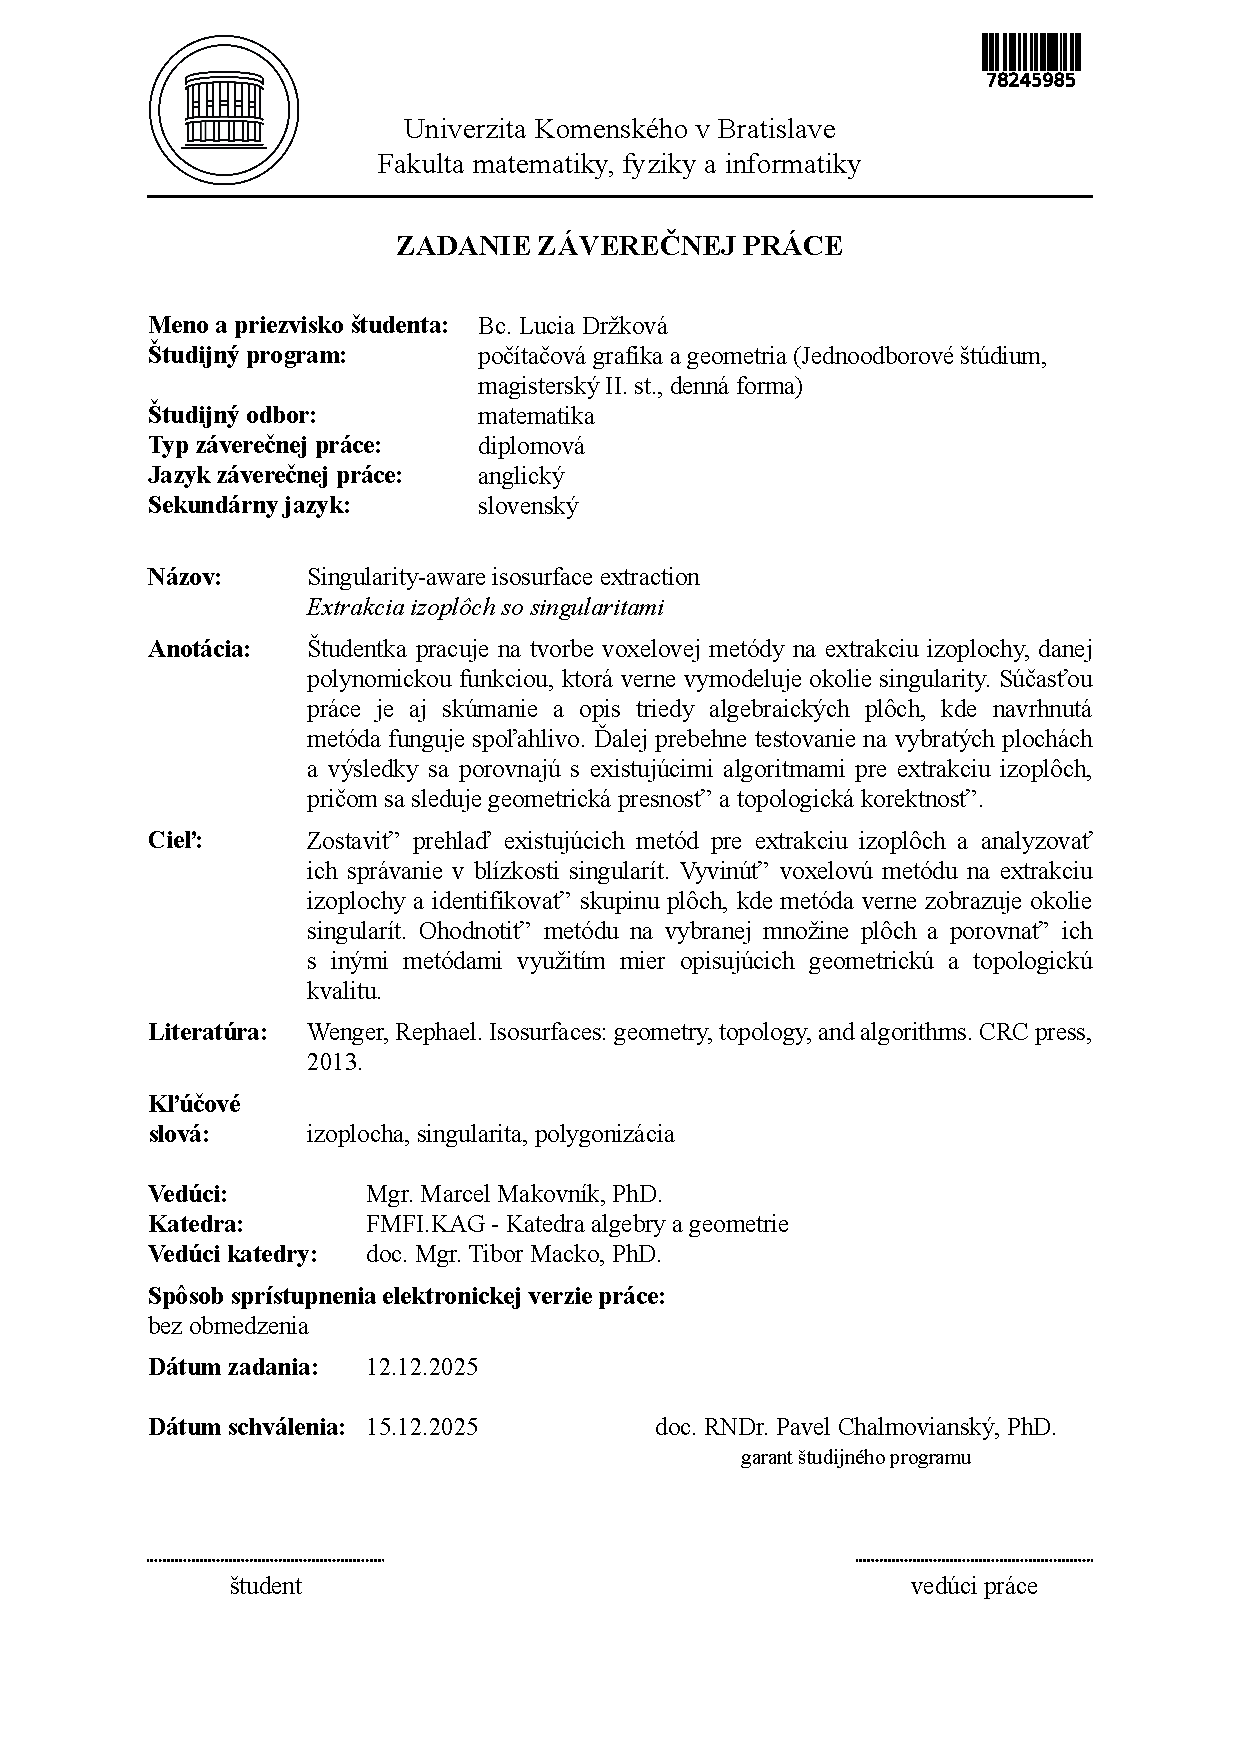
\includepdf[pages={1}]{zadanie-zp_209582.pdf}
 %\includepdf[pages={1}]{Zadanie_eng.pdf}
    
	\begin{titlepage} %čestné prehlásenie
    \section*{Declaration}

		\vspace*{\fill}
		{\setlength{\parindent}{0cm} 
        I hereby declare that I have independently completed the entire Master's thesis on the topic “Singularity-aware isosurface extraction” with the assistance of my supervisor, including all its appendices and illustrations, using only the literature listed in the attached bibliography and artificial intelligence tools. I declare that I have used artificial intelligence tools in accordance with the relevant legal regulations, academic rights and freedoms, ethical and moral principles, while maintaining academic integrity.} \\
		\flushright	........................................\\
	   Lucia Držková	
	\end{titlepage}



%%%%%%%%%%%%%%%%%%%%%%%%%%%%%%%%%%%%%%%%%%%%%%%%%%%%%%%%
% 														%
%  			 		Acknowledgement						%
% 														%
%%%%%%%%%%%%%%%%%%%%%%%%%%%%%%%%%%%%%%%%%%%%%%%%%%%%%%%%

% !!! OPTIONAL !!!
% However, it is nice gesture to give credit to all those who have helped you :-)
{~}\vfill
\section*{Acknowledgement}


	I want to thank...

\newpage

%%%%%%%%%%%%%%%%%%%%%%%%%%%%%%%%%%%%%%%%%%%%%%%%%%%%%%%%
% 														%
%  			 			Abstracts						%
% 														%
%%%%%%%%%%%%%%%%%%%%%%%%%%%%%%%%%%%%%%%%%%%%%%%%%%%%%%%%

% In english language
\section*{Abstract}
The text of abstract in English. \\

\noindent \textbf{keywords:} isosurface, singularity, polygonization

\newpage

% In slovak (national) language
\section*{Abstrakt}
Text abstraktu v slovenčine. \\

\noindent \textbf{kľúčové slová:} izoplocha, singularita, polygonizácia

\newpage

% All of the following are generated automatically

%%%%%%%%%%%%%%%%%%%%%%%%%%%%%%%%%%%%%%%%%%%%%%%%%%%%%%%%
% 														%
%  					Table of contents					%
% 														%
%%%%%%%%%%%%%%%%%%%%%%%%%%%%%%%%%%%%%%%%%%%%%%%%%%%%%%%%

\tableofcontents

%%%%%%%%%%%%%%%%%%%%%%%%%%%%%%%%%%%%%%%%%%%%%%%%%%%%%%%%
% 														%
%  					List of figures			 			%
% 														%
%%%%%%%%%%%%%%%%%%%%%%%%%%%%%%%%%%%%%%%%%%%%%%%%%%%%%%%%

\listoffigures

%%%%%%%%%%%%%%%%%%%%%%%%%%%%%%%%%%%%%%%%%%%%%%%%%%%%%%%%
% 														%
%  					List of tables			 			%
% 														%
%%%%%%%%%%%%%%%%%%%%%%%%%%%%%%%%%%%%%%%%%%%%%%%%%%%%%%%%

% !!! optional !!!
\listoftables
 
%%%%%%%%%%%%%%%%%%%%%%%%%%%%%%%%%%%%%%%%%%%%%%%%%%%%%%%%
% 														%
%  				List of source codes		 			%
% 														%
%%%%%%%%%%%%%%%%%%%%%%%%%%%%%%%%%%%%%%%%%%%%%%%%%%%%%%%% 
% !!! optional !!!
\lstlistoflistings % First pages -- mandatory !!!
\chapter*{Introduction} 
\addcontentsline{toc}{chapter}{Introduction} % the introduction is not numbered, since we have to add it to the table of contents manually
\pagenumbering{arabic} % starting with this page we use arabic page numbering

% the text of the introduction chapter % Introduction is an unnumbered chapter
\newpage

\chapter{Implicit Surfaces and Singularities}
\label{ch:implicit}


\section{Implicit Surfaces}
Implicit surfaces are defined as the set of points satisfying a scalar equation in three-dimensional space. They are used in computer graphics, geometric modeling, visualization, and numerical processing, and we will show their use in voxel-based methods and isosurface extraction algorithms \cite{bloomenthal2000implicit}.

\begin{definition}
\label{def:implicit-surface}
Let $f : \mathbb{R}^3 \to \mathbb{R}$ be a scalar-valued function. The set
\[
S = \{ p \in \mathbb{R}^3 \mid f(p) = 0 \}
\]
is called an \emph{implicit surface} or \emph{zero set} of the function $f$.
\end{definition}

The function $f$ is commonly referred to as the \emph{implicit surface function}. Beyond
identifying which points lie on the surface, the sign of $f$ classifies every point in
space according to its position relative to the surface:
\[
f(p) < 0 \quad \text{inside the surface},
\]
\[
f(p) > 0 \quad \text{outside the surface},
\]
\[
f(p) = 0 \quad \text{on the surface}.
\]

This classification property is one of the major advantages of implicit representations
over parametric approaches \cite{bloomenthal2000implicit}, as illustrated below.


\begin{figure}
    \centering
    \begin{center}
    \begin{tikzpicture}[scale=1.2, font=\small]
        \useasboundingbox (-3.5,-2) rectangle (3.5,2.5);
        \fill[blue!10] (0,0) circle (1.5);
        \draw[very thick, teal] (0,0) circle (1.5);
        \node[align=center] at (0,0) { $f(x,y,z) < 0$ \\ \scriptsize (Inside) };
        \draw[<-, thick] (1.06, 1.06) -- (2.2, 2) node[right, align=left] {
            $f(x,y,z) = 0$ \\
            \scriptsize (Surface $S$)
        };
        \node[align=center] at (2.5, -1) { $f(x,y,z) > 0$ \\ \scriptsize (Outside) };
    \end{tikzpicture}
    \end{center}
    \caption{Unit sphere with sign regions}
    \label{fig:unit_sphere}
\end{figure}


To see why this representation is useful, it is helpful to compare it with the two other
standard representations of surfaces. An explicit surface is represented as
$z=f(x,y)$, which restricts it to height-field configurations, while a parametric surface
defines each coordinate separately,
\[
x=f_x(s,t), \quad y=f_y(s,t), \quad z=f_z(s,t), \qquad (s,t)\in \text{parameter domain},
\]
giving direct access to points on the surface. Implicit surfaces instead treat all
coordinates symmetrically, which allows more complex geometric structures and naturally
supports merging, blending, and deformation operations \cite{bloomenthal2000implicit}.

A natural question is when an implicit surface can locally be described as a smooth
two-dimensional object. This is answered by the following classical result.

\begin{theorem}
Let $f : \mathbb{R}^3 \to \mathbb{R}$ be continuously differentiable in a neighborhood of
a point $p=(x_0,y_0,z_0)$ with $f(p)=0$. If at least one partial derivative of $f$ is
nonzero at $p$, then locally the surface can be expressed as an explicit function of two
variables.
\end{theorem}

The theorem guarantees local regularity whenever the gradient does not vanish, which
motivates the following distinction.

\begin{definition}
\label{def:regular-singular}
A point $p$ on an implicit surface is called a \emph{regular point} if
$\nabla f(p)\neq 0$. Otherwise, $p$ is called a \emph{singular point}.
\end{definition}

The gradient
\[
\nabla f(x,y,z)=
\left(
\frac{\partial f}{\partial x},
\frac{\partial f}{\partial y},
\frac{\partial f}{\partial z}
\right)
\]
defines the local differential structure of the surface and its normal direction. At
regular points this direction is well-defined and the surface locally resembles a smooth
plane; at singular points this structure may break down entirely, which we discuss in
Section~\ref{sec:singularities}.

The most analytically tractable implicit surfaces are those defined by polynomial
functions.

\begin{definition}
An implicit surface is called an \emph{algebraic surface} if the defining function $f$
is polynomial.
\end{definition}

Algebraic surfaces are especially relevant for singularity analysis, because polynomial
structure allows local geometric behavior to be studied through algebraic methods.

An important practical property of implicit surfaces is their suitability for polygonization and voxel-based processing: since the surface is represented by samples of a scalar field, algorithms such as Marching Cubes or Dual Contouring can reconstruct polygonal approximations directly from volumetric data, which makes implicit representations well suited for scientific visualization, medical imaging, and adaptive
geometric modeling \cite{bloomenthal2000implicit}. This combination of algebraic
structure, differential properties, and numerical flexibility is what makes implicit
surfaces a natural framework for studying singularity-aware isosurface extraction, the
topic to which the rest of this chapter is devoted.

\section{Differential and Algebraic Properties of Implicit Surfaces}

Having introduced implicit surfaces as zero sets of a scalar function
$f:\mathbb{R}^3 \rightarrow \mathbb{R}$, we now examine their differential properties in
more detail, starting with the gradient.

\subsection{Gradient and Normal Vector}

The gradient of $f$ is the primary tool for extracting geometric information from an
implicit surface: it encodes how the scalar field changes in each spatial direction and
points perpendicularly to the level set of $f$.

\begin{definition}%[Implicit Surface Gradient]
Let $f(x,y,z)$ be a differentiable scalar field. The gradient of $f$ is
\[
\nabla f(x,y,z) = \left(\frac{\partial f}{\partial x}, \frac{\partial f}{\partial y},
\frac{\partial f}{\partial z}\right).
\]
\end{definition}

\begin{theorem}%[Surface Normal]
If $\nabla f(p) \neq 0$, then the unit normal vector to the implicit surface at $p$ is
\[
\mathbf{n}(p) = \frac{\nabla f(p)}{\|\nabla f(p)\|}.
\]
\end{theorem}

Recall from Definition~\ref{def:regular-singular} that regular points admit a
well-defined normal direction, whereas singular points may not. We next examine how this
translates into the existence of a tangent plane.

\subsection{Tangent Planes and Local Smoothness}

\begin{definition}%[Tangent Plane]
At a regular point $p_0$ on the implicit surface $f(x,y,z)=0$, the tangent plane is
given by
\[
\nabla f(p_0) \cdot (p - p_0) = 0.
\]
\end{definition}

A non-zero gradient therefore ensures local smoothness, and if $f$ is continuously
differentiable, the implicit surface is locally a smooth 2-manifold
\cite{bloomenthal2000implicit}. Beyond this first-order behavior, second-order
derivatives determine how the surface curves.

\subsection{Curvature and Local Geometric Behavior}

\begin{definition}%[Curvature Behavior]
The curvature of an implicit surface is governed by the second-order derivatives of $f$, and is well-defined when $f$ is twice continuously differentiable and $\nabla f \neq 0$.
\end{definition}

Smooth implicit surfaces are therefore classified as $G^2$ continuous under appropriate regularity conditions \cite{bloomenthal2000implicit}. This regularity breaks down at singular points, where the gradient vanishes; we examine such points in detail in Section~\ref{sec:singularities}. As a first illustration, consider the cone
\[
f(x,y,z) = -x^2 + y^2 + z^2,
\]
whose apex at the origin is a singular point where the gradient vanishes, producing a degenerate geometric structure \cite{bloomenthal2000implicit} (Figure~\ref{fig:cone}).

\begin{figure}[!h]
    \centering
    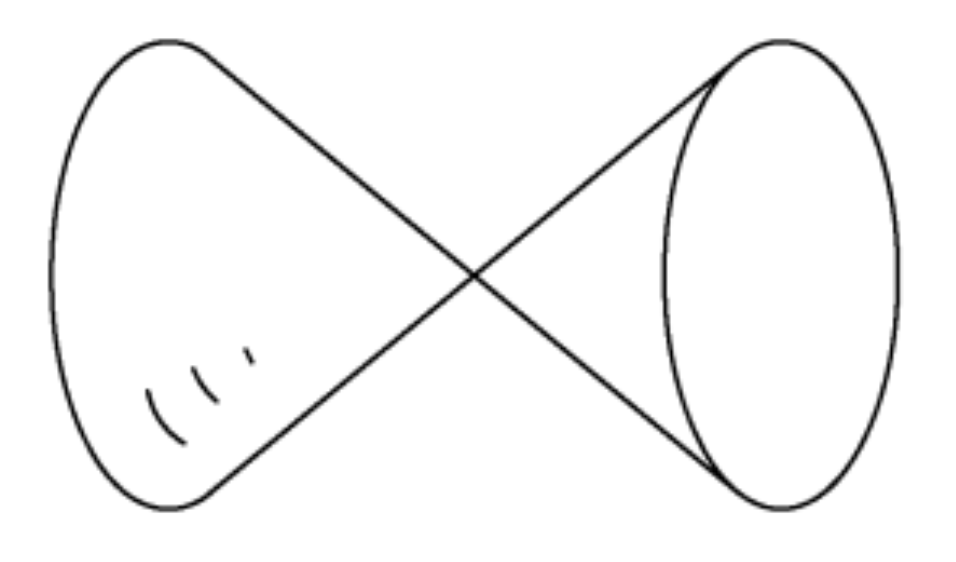
\includegraphics[width=0.4\textwidth]{pictures/cone.png}
    \caption[Cone singularity]{The apex of a cone is a singular point (image retrieved
    from \cite{bloomenthal2000implicit}).}
    \label{fig:cone}
\end{figure}

\subsection{Algebraic Multiplicity and Geometric Behavior}

The algebraic degree of the function $f$ appears to influence the geometry such as the number of intersections with other objects and the local geometry of algebraic surfaces. In general, surfaces with larger degrees will have more complex curvature and singular behaviour. A key relationship between algebraic and geometric structure is that higher algebraic multiplicity at a point may correspond to degeneracies or singularities in the geometry of the surface \cite{bloomenthal2000implicit}.

The following result of this section summarizes the ideas which have been developed on implicit surfaces, leading to a clean sufficient condition for an implicit surface to be a smooth manifold.

% [Manifold Condition]
\begin{theorem}
\label{thm:manifold}
If $f$ is continuously differentiable and $0$ is a regular value of $f$, then the implicit surface $f^{-1}(0)$ is a 2-dimensional manifold embedded in $\mathbb{R}^3$.
\end{theorem}

This result ensures that, under regularity conditions, implicit surfaces behave as smooth geometric objects with well-defined local structure. The following section investigates what happens when this regularity fails.

\section{Singularities of Implicit Surfaces}
\label{sec:singularities}

Recall that a point $p$ on an implicit surface $S=\{p \mid f(p)=0\}$ is \emph{singular} if $\nabla f(p) = 0$ (Definition~\ref{def:regular-singular}). By Theorem~\ref{thm:manifold}, singular points are precisely those where $S$ may fail to be locally manifold-like, since the surface normal and tangent plane are no longer well-defined there. We now study the geometric and numerical consequences of this condition systematically.

\subsection{Isolated and Non-Isolated Singular Points}
\label{sec:isolated}

Singular points do not have to be single points. They can also form whole curves on the surface, and the two situations behave very differently, both in theory and in numerical computation.

\begin{definition}
\label{def:isolated}
A singular point $p$ of the implicit surface $S=\{f=0\}$ is called \emph{isolated} if there is a neighbourhood $U$ of $p$ such that $p$ is the only singular point of $S$ in $U$.
\end{definition}

The apex of the cone in Figure~\ref{fig:cone} is isolated, since the gradient $\nabla f=(-2x,2y,2z)$ vanishes only at the origin. A standard example of a non-isolated singularity is the Whitney umbrella $f(x,y,z)=x^2-y^2z$ \cite{umehara2022differential}. Its gradient $(2x,-2yz,-y^2)$ vanishes on the whole $z$-axis, and every point of the axis lies on the surface, so the surface is singular along a line. In this thesis we work only with isolated singular points.

The local shape of a surface near a singular point is described, as a first approximation, by the lowest-order terms of $f$.

\begin{definition}
\label{def:tangent-cone}
Let $f$ be a polynomial with $f(p)=0$ and write
\[
f(p+u)=f_m(u)+f_{m+1}(u)+\dots,
\]
where $f_j$ is a homogeneous polynomial of degree $j$ and $f_m\neq0$. The number $m$ is called the \emph{multiplicity} of $f$ at $p$, and the zero set $\{u\in\mathbb{R}^3 \mid f_m(u)=0\}$ is called the \emph{tangent cone} of $S$ at $p$ \cite{dimca1992singularities}.
\end{definition}

A point is regular exactly when $m=1$, and then the tangent cone is the tangent plane. At a singular point $m\ge2$, which is the higher algebraic multiplicity mentioned in the previous section. For the cone $f=-x^2+y^2+z^2$ the tangent cone is the surface itself. For $f=x^2+y^2+z^3$ the tangent cone is $\{x^2+y^2=0\}$, which in $\mathbb{R}^3$ is only the $z$-axis and says nothing about the actual shape of the surface, a thin horn (Chapter~\ref{ch:experiments}). For such surfaces the ordinary degree has to be replaced by a weighted degree (Definition~\ref{def:quasihomogeneous}).

\subsection{Non-Degenerate Singular Points and the Morse Lemma}

The Morse lemma describes the local behaviour of a smooth function near a non-degenerate critical point. A point $P$ is a critical point of a function $F$ if $\nabla F(P)=0$. It is called \emph{non-degenerate} if its Hessian matrix is invertible, that is,
\[
\det(\operatorname{Hess}F(P))\neq 0.
\]

\begin{theorem}[Morse lemma \cite{milnor1963morse}]
\label{thm:morse}
Let $F:U\to\mathbb R$ be a smooth function, where $U\subseteq\mathbb R^n$ is an open set, and let $P\in U$ be a non-degenerate critical point of $F$. Then there exists a local coordinate system $(u_1,\dots,u_n)$ centered at $P$ in which
\[
F=F(P)-u_1^2-\cdots-u_\lambda^2+u_{\lambda+1}^2+\cdots+u_n^2,
\]
where $\lambda$ is the number of negative eigenvalues of the Hessian of $F$ at $P$, counted with multiplicity.
\end{theorem}

In other words, near a non-degenerate critical point the function can be represented by a quadratic expression after a suitable change of coordinates, and the signs of the quadratic terms are determined by the Hessian. For a surface $\{F=0\}$ in $\mathbb{R}^3$ with $F(P)=0$ there are only two real possibilities. If $\lambda=0$ or $\lambda=3$, the surface near $P$ is $u_1^2+u_2^2+u_3^2=0$, a single isolated point. If $\lambda=1$ or $\lambda=2$, it is $u_1^2+u_2^2-u_3^2=0$ (up to the order of the coordinates), a double cone.

\begin{example}
\label{ex:morse}
For the surface
\[
F(x,y,z)=x^2+y^2-z^2+xyz,
\]
the Hessian at the origin is
\[
\operatorname{Hess}F(0,0,0)=
\begin{pmatrix}
2&0&0\\
0&2&0\\
0&0&-2
\end{pmatrix}.
\]
Since this matrix is invertible, the origin is a non-degenerate critical point. By the Morse lemma, the equation is locally equivalent to $u^2+v^2-w^2=0$, so near the origin the surface is a double cone. In the notation introduced below, the origin is an $A_1$ singularity.
\end{example}

\subsection{Milnor and Tjurina Numbers}

When the Hessian is not invertible, the singular point is degenerate and the Morse lemma does not apply. The degree of degeneracy is then measured by two numbers from singularity theory. Let $\mathcal{O}$ denote the ring of convergent power series in $x,y,z$ near the origin; for example, expressions such as $1+x^2+y^2+xz+z^3+\dots$ belong to this ring. All singular points below are moved to the origin by a translation.

\begin{definition}[Milnor and Tjurina numbers \cite{milnor1968singular,greuel2007introduction}]
\label{def:milnor}
Let $F\in\mathcal{O}$ with $F(0)=0$. The \emph{Milnor algebra} and the \emph{Tjurina algebra} of $F$ at the origin are
\[
M_F=\mathcal{O}\big/\big(\partial_xF,\partial_yF,\partial_zF\big),\qquad
T_F=\mathcal{O}\big/\big(F,\partial_xF,\partial_yF,\partial_zF\big),
\]
and their dimensions as vector spaces are the \emph{Milnor number} $\mu(F)$ and the \emph{Tjurina number} $\tau(F)$.
\end{definition}

The quotient means that two power series are treated as equal if they differ by a combination of the partial derivatives (and, for $T_F$, of $F$ itself). For the surface $F=x^2+y^2+z^3$ the partial derivatives are $2x$, $2y$ and $3z^2$. Every power series is, modulo these three, equal to a combination of $1$ and $z$, so $M_F$ is spanned by $1$ and $z$ and $\mu=2$. For the double point of Example~\ref{ex:morse} the linear parts $2x$, $2y$, $-2z$ of the partial derivatives allow us to remove every term containing $x$, $y$ or $z$, so only the constant remains and $\mu=1$.

\begin{theorem}[\cite{greuel2007introduction}]
\label{thm:mu-finite}
The Milnor number $\mu(F)$ is finite if and only if the origin is an isolated zero of $\nabla F$ in $\mathbb{C}^3$.
\end{theorem}

If $\mu(F)<\infty$, the origin is in particular an isolated singular point of the real surface. The converse does not hold: $F=(x^2+y^2)^2+z^2$ has only the real critical point $0$, but over the complex numbers $\nabla F$ vanishes on the curve $\{x^2+y^2=0,\ z=0\}$, so $\mu=\infty$. All surfaces in this thesis have a finite Milnor number.

A special role is played by polynomials that become homogeneous once every variable is given its own weight.

\begin{definition}
\label{def:quasihomogeneous}
A polynomial $F$ is \emph{quasi-homogeneous} (or weighted homogeneous) with weights $w=(w_x,w_y,w_z)$, $w_x,w_y,w_z>0$, if
\[
F(t^{w_x}x,t^{w_y}y,t^{w_z}z)=t\,F(x,y,z)\qquad\text{for all }t>0.
\]
The \emph{weighted degree} of a monomial $x^ay^bz^c$ is $d_w(x^ay^bz^c)=aw_x+bw_y+cw_z$, so $F$ is quasi-homogeneous exactly when all its monomials have weighted degree $1$.
\end{definition}

A homogeneous polynomial of degree $d$ is quasi-homogeneous with all weights equal to $1/d$. The polynomial $x^2+y^2+z^3$ is quasi-homogeneous with the weights $(\tfrac12,\tfrac12,\tfrac13)$: shrinking $x$ and $y$ by $t^{1/2}$ and $z$ by $t^{1/3}$ scales every term by the same factor $t$.

\begin{theorem}[Saito \cite{saito1971quasihomogene}]
\label{thm:saito}
Let $F$ have an isolated singular point at the origin. Then $\tau(F)\le\mu(F)$, and $\tau(F)=\mu(F)$ if and only if $F$ is quasi-homogeneous in suitable local coordinates.
\end{theorem}

For quasi-homogeneous polynomials the Milnor number can even be read off from the weights alone.

\begin{theorem}[Milnor and Orlik \cite{milnor1970isolated}]
\label{thm:milnor-orlik}
Let $F$ be quasi-homogeneous with weights $w=(w_x,w_y,w_z)$ and with an isolated singular point at the origin. Then
\[
\mu(F)=\Big(\frac{1}{w_x}-1\Big)\Big(\frac{1}{w_y}-1\Big)\Big(\frac{1}{w_z}-1\Big).
\]
\end{theorem}

For $x^2+y^2+z^3$ this gives $1\cdot1\cdot2=2$, in agreement with the computation above, and for a homogeneous cubic with an isolated singular point it gives $2\cdot2\cdot2=8$.

\subsection{Normal Forms}

Two polynomials that look different can describe the same singular point after a change of coordinates. We say that two germs $F$ and $\tilde F$ at the origin are \emph{right equivalent} if there is a local diffeomorphism $\Psi$ with $\Psi(0)=0$ and $\tilde F=F\circ\Psi$. The Milnor and Tjurina numbers do not change under right equivalence \cite{greuel2007introduction}, and isolated singular points are classified up to right equivalence by \emph{normal forms}, the simplest equations in each class.

\begin{theorem}[Arnold \cite{arnold1985singularities}]
\label{thm:simple}
The simple singularities of functions of three variables are, up to right equivalence over $\mathbb{C}$ and up to adding squares of further variables,
\[
A_k:\ x^{k+1}+y^2+z^2\ (k\ge1),\qquad
D_k:\ x^2y+y^{k-1}+z^2\ (k\ge4),
\]
\[
E_6:\ x^3+y^4+z^2,\qquad E_7:\ x^3+xy^3+z^2,\qquad E_8:\ x^3+y^5+z^2 .
\]
The index is the Milnor number: $\mu(A_k)=\mu(D_k)=\mu(E_k)=k$.
\end{theorem}

Over the real numbers each class splits further according to the signs of the terms. Our ten test surfaces have four types, listed in Table~\ref{tab:normal-forms}.

\begin{table}[!h]
\centering
\small
\begin{adjustbox}{max width=\textwidth}
\begin{tabular}{l l c c l}
\toprule
Type & Normal form & $\mu$ & Weights $(w_x,w_y,w_z)$ & What it looks like \\
\midrule
$A_1$ & $x^2+y^2-z^2$ & $1$ & $(\frac12,\frac12,\frac12)$ & double cone \\
$A_2$ & $x^2\pm y^2+z^3$ & $2$ & $(\frac12,\frac12,\frac13)$ & cusp: a horn or a pinched saddle \\
$D_4$ & $x^2+y^3+z^3$, \ $x^2+y^3-3yz^2$ & $4$ & $(\frac12,\frac13,\frac13)$ & one or three pieces pinched along lines \\
$\tilde E_6$ & $x^3+y^3+z^3+t\,xyz$, \ $t^3\neq-27$ & $8$ & $(\frac13,\frac13,\frac13)$ & a cone over a cubic curve \\
\bottomrule
\end{tabular}
\end{adjustbox}
\caption[Normal forms]{Normal forms of the singularity types used in this thesis \cite{arnold1985singularities,arnold2012singularities}. Over the real numbers $A_2$ and $D_4$ have several forms that differ by signs.}
\label{tab:normal-forms}
\end{table}

The labels $A_1$, $A_2$, $D_4$ and $\tilde E_6$ describe the local algebraic structure of a singular point. Type $A_1$ represents an ordinary double point. Its quadratic part is non-degenerate, and the set of its real zeros can take the form of a double cone, as in Example~\ref{ex:morse}. Type $A_2$ represents a cusp-type singularity with the normal form $x^2\pm y^2+z^3$. The sign of the quadratic part determines the real geometry: a positive definite form gives a thin horn ending in a tip, whereas an indefinite form gives a configuration resembling a saddle. Type $D_4$ has a normal form consisting of a quadratic term and a cubic polynomial in the remaining variables, for example $x^2+y^3-3yz^2$. The cubic part may contain one or three distinct real lines through the origin. This changes the real appearance of the surface, even though the algebraic type remains $D_4$.

The type $\tilde E_6$ describes a cone over a smooth homogeneous cubic curve. Its defining polynomial is homogeneous of degree three, and the singular point at the origin has the Milnor number $\mu=8$. It is not a simple singularity: it comes in a one-parameter family, because the modulus of the elliptic curve cannot be changed by coordinate changes \cite{arnold1985singularities}. It should not be confused with the simple singularity $E_6$, whose normal form is $x^3+y^4+z^2$ and whose Milnor number is $6$. Among the isolated singular points of cubic surfaces, $\tilde E_6$ is the most degenerate one; the others are $A_1,\dots,A_5$, $D_4$, $D_5$ and $E_6$ \cite{bruce1979classification}.

\subsection{Local Topology: the Conic Structure Theorem}
\label{sec:conic}

The last result of this section describes the topology of a surface near a singular point, whatever its type. For $\varepsilon>0$ let $B_\varepsilon(p)$ be the closed ball and $\partial B_\varepsilon(p)$ the sphere of radius $\varepsilon$ around $p$.

\begin{theorem}[Conic structure theorem, Milnor \cite{milnor1968singular}]
\label{thm:conic}
Let $V\subset\mathbb{R}^n$ be a real algebraic set and $p\in V$. For every sufficiently small $\varepsilon>0$ the intersection $V\cap B_\varepsilon(p)$ is homeomorphic to the cone over the \emph{link} $K=V\cap\partial B_\varepsilon(p)$, that is, to the union of all segments joining $p$ with the points of $K$.
\end{theorem}

If $p$ is an isolated singular point of a surface in $\mathbb{R}^3$, the link $K$ is, for small $\varepsilon$, a finite union of disjoint closed curves \cite{milnor1968singular}. The link of the double cone consists of two circles, one for each nappe. The link of the horn $x^2+y^2+z^3$ is a single circle, and so is the link of the Fermat cone $x^3+y^3+z^3$ (Chapter~\ref{ch:experiments}).

\begin{corollary}
\label{cor:cone-topology}
Under the assumptions of Theorem~\ref{thm:conic}, $V\cap B_\varepsilon(p)$ is connected and contractible, and its Euler characteristic is $\chi=1$, however many components the link has.
\end{corollary}

\begin{proof}
A cone over any space is contractible, since it can be shrunk to its apex along the segments. A contractible space is connected and has the Euler characteristic of a point, which is $1$ \cite{hatcher2002algebraic}.
\end{proof}

This simple fact is the basis of the topological evaluation in this thesis: a correct mesh of the surface in a small box around an isolated singular point must be connected and must have $\chi=1$. A mesh in which the two nappes of a double cone do not touch has two components and $\chi=2$ instead. Besides describing a singular point as it is, one can also try to resolve it, which is the subject of the next section, or perturb it, which is studied in Section~\ref{sec:unfolding} and in Chapter~\ref{ch:theory}.

\begin{comment}
\subsection{Geometric Interpretation of Singularities}

Geometrically, singularities correspond to locations where the surface loses local flatness, changes topology, or exhibits self-degeneracy, as in the cone example of Figure~\ref{fig:cone}. Such behavior is crucial in both theoretical geometry and numerical computation, as it affects stability in surface reconstruction and rendering algorithms \cite{bloomenthal2000implicit}. These degeneracies occur in several qualitatively distinct forms, which are classified below.


\subsection{Types of Singular Behavior}

These forms are best understood using the singularity theory of smooth mappings, which classifies them via local normal forms \cite{arnold2012singularities}.

\begin{definition}[Types of singular behavior]
The following local forms are commonly encountered:
\begin{itemize}
    \item \textbf{Cusp}: a smooth curve or surface locally forms a pointed tip,
          typically from higher-order degeneracy of derivatives.
    \item \textbf{Swallowtail}: a higher-order singularity with self-intersecting local
          structure and a curvature-sign change in multiple directions.
    \item \textbf{Pinch point}: two local sheets of a surface touch tangentially
          without forming a smooth intersection.
    \item \textbf{Higher-order degeneracy}: not only the first derivative but also
          higher-order derivatives vanish or become linearly dependent, producing
          complex local geometry.
\end{itemize}
\end{definition}

These types can also be distinguished according to whether they affect only a small
neighborhood of a point or the global topology of the surface.

\subsection{Local versus Global Singular Structure}

\begin{itemize}
    \item \textbf{Local singularities} depend only on the behavior of $f$ in an
          infinitesimal neighborhood of a point.
    \item \textbf{Global singularities} affect the topology of the entire surface, such
          as self-intersections or disconnected components.
\end{itemize}

While local singularities determine differential properties, global singular structures
influence the topology and connectivity of the implicit surface. Beyond their theoretical
interest, singularities have direct consequences for numerical methods that reconstruct
implicit surfaces from sampled data.

\subsection{Numerical Difficulties in Polygonization}

Numerical procedures rely on the gradient to estimate normals and classify voxel cells,
and both operations become unreliable when the gradient is close to zero. Near such
points, numerical methods may fail due to unstable normal estimation, ambiguous cell
classification, missed or duplicated surface components, and incorrect topology
reconstruction.

\begin{theorem}[Numerical Instability Near Singularities]
Let $S = \{p \mid f(p)=0\}$ be an implicit surface and let $p_s$ be a singular point such
that $\nabla f(p_s)=0$. Then numerical approximation of the surface normal and local
topology near $p_s$ becomes ill-conditioned.
\end{theorem}

This instability is a fundamental limitation of discrete polygonization methods and
motivates adaptive refinement techniques and alternative implicit evaluation strategies
\cite{bloomenthal2000implicit}.

\subsection*{Summary}

Singularities represent points where the standard manifold structure of an implicit
surface fails, producing both rich geometric phenomena (cusps, swallowtails, pinch
points) and significant numerical challenges. The next two sections address,
respectively, how such singularities can be resolved theoretically, and how they behave
under perturbation; Chapter 2 then turns to how numerical algorithms can be made more
robust in their presence.

\section{Blowup and Resolution of Singularities}

A natural question is whether singularities can be systematically resolved, that is, replaced by a smoother structure capturing the same geometric information without the degeneracy. Consider the context of piecewise smooth dynamical systems. For non-unique singularities such as the visible-invisible two-fold, the non-uniqueness suggests geometric desingularization methods such as regularization and blowup. These ideas are developed systematically in \cite{kristiansen2019resolution}, which combines geometric singular perturbation theory with blowup techniques to resolve non-hyperbolic behavior.

\begin{definition}%[Motivation for desingularization]
Let $X^\pm$ define a piecewise smooth vector field with switching manifold $\Sigma = \{y=0\}$. A singularity $q \in \Sigma$ is called \emph{non-deterministic} if the associated Filippov flow is not uniquely defined at $q$. Desingularization embeds the PWS system into a smooth family $X_\epsilon$ such that the limiting dynamics as $\epsilon \to 0^+$ recover the original system while resolving forward non-uniqueness.
\end{definition}

The central tool is the blowup transformation, which replaces a singular point with a
higher-dimensional manifold capturing directional information of the flow, separating
the different directions from which trajectories can approach it.

\begin{definition}[Blowup in $\mathbb{R}^3$]
Consider a singular point $y=\epsilon=0$. The blowup transformation introduces
polar-type coordinates
\[
(y,\epsilon) = \rho(\bar{y}, \bar{\epsilon}), \quad (\bar{y},\bar{\epsilon}) \in S^1,
\ \rho \geq 0,
\]
where $S^1 = \{(\bar{y},\bar{\epsilon}) \in \mathbb{R}^2 \mid \bar{y}^2 +
\bar{\epsilon}^2 = 1\}$. Under this transformation, the singular point is replaced by the
circle $S^1$, which encodes all possible directional approaches to the singularity.
\end{definition}

\begin{theorem}[Resolution via blowup and regularization \cite{kristiansen2019resolution}]
Let $X_\epsilon$ be a regularized PWS system near a visible--invisible two-fold
singularity $q$. Then, under the blowup transformation and appropriate directional
charts, the system admits a desingularized vector field $X$ on the blown-up space.
Moreover:
\begin{itemize}
    \item The singular two-fold point $q$ lifts to a circle of equilibria
          $\bar{q} \cong S^1$.
    \item The dynamics near $\bar{q}$ separates into invariant directional charts
          corresponding to different asymptotic regimes.
    \item Stable and unstable sliding regions of the original system correspond to
          normally hyperbolic invariant manifolds in the blown-up space.
    \item Loss of hyperbolicity at folds and two-folds becomes a geometric degeneracy
          that can be resolved via local analysis in directional charts.
\end{itemize}
Consequently, forward evolution through the singularity can be uniquely extended in the
regularized system.
\end{theorem}

To work concretely within the blown-up space, one introduces directional charts such as
\[
(y,\epsilon) = (\epsilon \hat{y}, \epsilon) \quad \text{or} \quad (y,\epsilon) =
(y, y \hat{\epsilon}),
\]
which correspond to different regions of the blown-up sphere and allow the desingularized
vector field to be expressed using standard dynamical systems tools. In the
visible--invisible two-fold, for instance, trajectories entering the singularity are
lifted to trajectories on the blown-up circle, where invariant objects such as canards
and sliding flows become separated into distinct geometric objects that can be studied in
a regular setting. In summary, the blowup method shows that singular dynamics in the
original PWS system can be reinterpreted as smooth dynamics on a higher-dimensional
manifold, where local topology is preserved under regularization while the fine structure
of trajectories near the two-fold is governed by invariant manifolds in the blown-up
space \cite{kristiansen2019resolution}.
\end{comment}

\section{Blowup and Resolution of Singularities}
\label{sec:blowup}

The analysis of piecewise smooth (PWS) systems near non-unique singularities, such as the visible–invisible two-fold, requires techniques capable of resolving degeneracies where trajectories lack unique forward evolution. In these systems, trajectories entering a two-fold point are associated with forward non-uniqueness, posing the question of how to continue orbits forward in time. To address this, a combination of regularization and geometric blowup is used to resolve the non-deterministic behavior \cite{kristiansen2019resolution}.

\subsection{Regularization and the Singular System}

Mathematically, a PWS system in $\mathbb{R}^n$ is defined by smooth vector fields $X^+$ and $X^-$ separated by a switching manifold $\Sigma = \{x : y = 0\}$. A regularization is introduced to replace the discontinuous system with a smooth one that recovers the original dynamics as $\epsilon \to 0$:

\begin{equation}
    X_\epsilon(x) = \frac{1}{2}X^+(x)(1 + \phi(\epsilon^{-1}y)) + \frac{1}{2}X^-(x)(1 - \phi(\epsilon^{-1}y)),
\end{equation}

where $\phi$ is a smooth, monotone regularization function. This process introduces a singular point at $\epsilon = 0$, where the vector field is not immediately well-defined in the limit.

\subsection{The Blowup Transformation}

The blowup transformation is a desingularization method that replaces the singular point with a higher-dimensional manifold, such as a circle or sphere, to capture the directional information of the flow. By "blowing up" the point $x=0$, trajectories that were collapsed at the singularity become separated on the new manifold, allowing for a detailed study of their transitions \cite{kristiansen2019resolution}.

\begin{definition}
Given a vector of positive integers $\alpha = (\alpha_1, \dots, \alpha_n)$ called weights, the weighted (or quasihomogeneous) blowup transformation is a mapping $\pi: [0, \infty) \times S^{n-1}_{\alpha} \to \mathbb{R}^n$ defined by:

\begin{equation}
    (\rho, \bar{x}) \mapsto x = (\rho^{\alpha_1} \bar{x}_1, \dots, \rho^{\alpha_n} \bar{x}_n),
\end{equation}

where $S^{n-1}_{\alpha}$ is the unit $\alpha$-sphere.
\end{definition}

For the visible–invisible two-fold, the transformation blows up the singularity to the unit circle \cite{kristiansen2019resolution}.

\begin{figure}[!h]
    \centering
    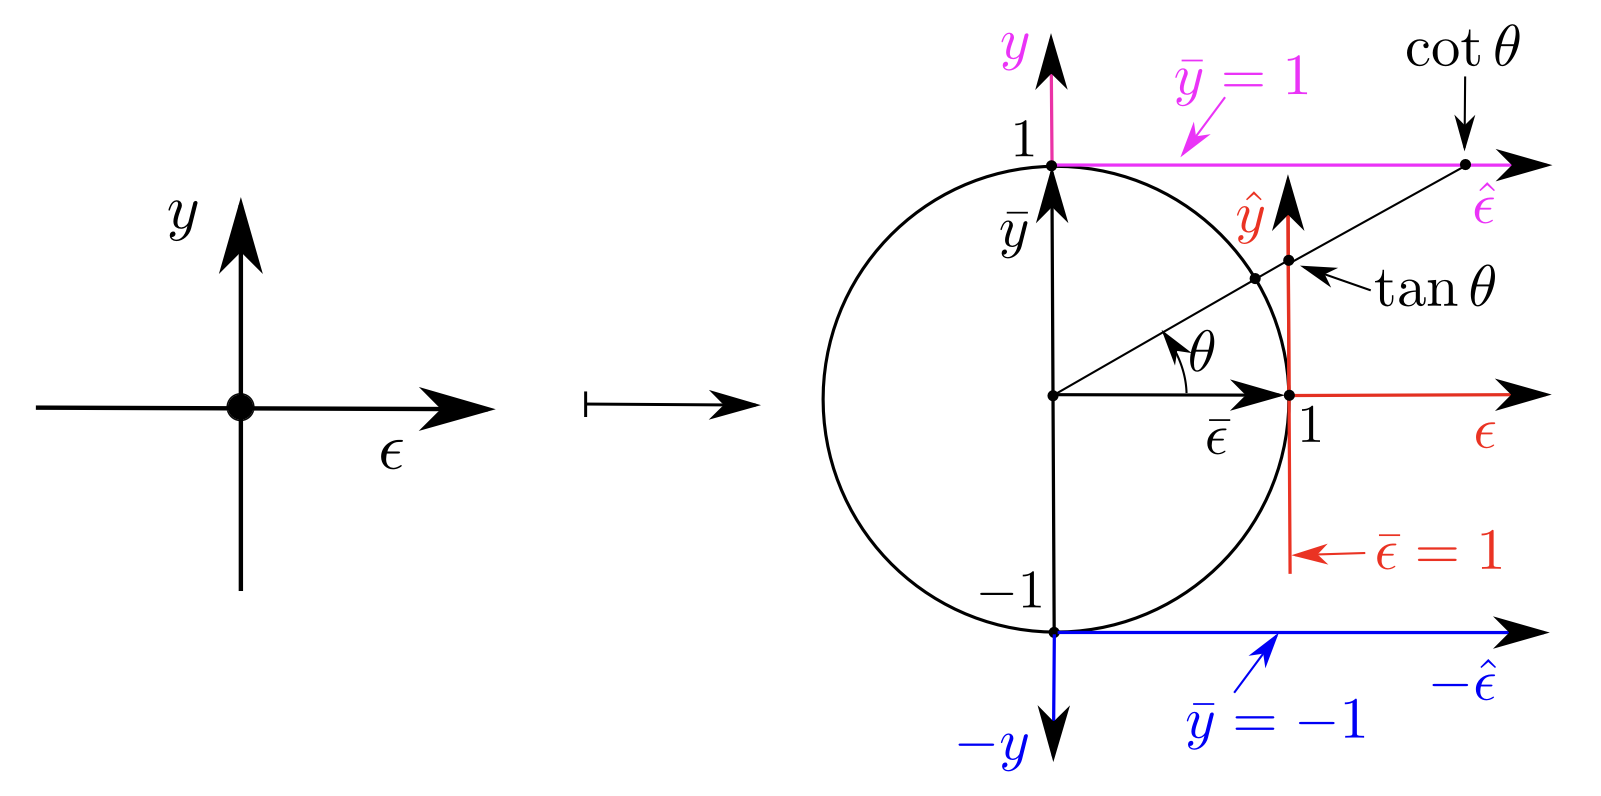
\includegraphics[width=0.6\textwidth]{pictures/blowup.png}
    \caption[Blowup]{Blowup of $y= \epsilon =0$ to the unit circle $y^2+\epsilon^2=1 $. Charts $\epsilon=1$, $y=1$ and $y=-1$ in the blowup transformation (image retrieved
    from \cite{kristiansen2019resolution}).}
    \label{fig:blowup}
\end{figure}


\subsection{Directional Charts and Coordinates}

To analyze the dynamics on the blown-up manifold, the system is expressed in directional charts, which provide an atlas with smooth coordinate changes between overlapping regions. These charts are obtained by setting a specific directional variable to a constant \cite{kristiansen2019resolution}.

\begin{itemize}
    \item \textbf{Chart $K_i^+$:} Defined by the mapping $\bar{x}_i = 1$.
    \item \textbf{Chart $K_i^-$:} Defined by $\bar{x}_i = -1$.
\end{itemize}

These coordinate transformations allow the desingularized vector field to be studied using standard tools of geometric singular perturbation theory.

\subsection{Geometric Resolution and Results}

The main purpose of the process is the determination whether there exist special orbits in the set of possible orbits that have the capacity to evolve further. As far as Kristiansen and Hogan \cite{kristiansen2019resolution} analyze the regularized visible-invisible two-fold, they prove an important technical lemma about the transition through the singular point. Under some conditions, the forward flow of the regularized system possesses a transition map between sections of the phase space that is defined and $C^1$ for all sufficiently small $\epsilon > 0$.

The blowup analysis reveals that there is indeed a unique distinguished forward orbit that characterizes the transition from the two-fold. In this framework, singular dynamics are transformed into smooth dynamics on the higher-dimensional manifold, providing a rigorous geometric foundation for continuing orbits forward in time \cite{kristiansen2019resolution}.

\section{Unfolding and Stability}
\label{sec:unfolding}

The concepts of unfolding and stability are central to understanding how singular structures, such as implicit surfaces or dynamical systems, behave under perturbation. While unfolding in a mathematical sense describes the qualitative changes in a system's behavior near a singularity, structural stability refers to the persistence of its qualitative behavior under small perturbations \cite{ibanez2005shil}.

\subsection{Mathematical Unfolding of Singularities}

An unfolding, in singularity theory and dynamical systems, is a parameterized family of systems which includes a singular (non-structurally stable) one. A system is defined as structurally stable if it lies within the interior of its equivalence class in a topology on a set of dynamical systems. The collection of all non-structurally stable systems is called the bifurcation set \cite{ibanez2005shil}.

For a nilpotent singularity of codimension three in $\mathbb{R}^3$, the vector field $X$ vanishes at the origin with a linear part conjugate to:
\begin{equation}
    J = \begin{pmatrix} 0 & 1 & 0 \\ 0 & 0 & 1 \\ 0 & 0 & 0 \end{pmatrix}.
\end{equation}
Any generic three-parameter unfolding $X_\Lambda$ with parameters $\Lambda = (\lambda_1, \lambda_2, \lambda_3)$ can be expressed in the following normal form:

\begin{equation}
    y \frac{\partial}{\partial x} + z \frac{\partial}{\partial y} + (\lambda + my + nz + x^2 + bxy + cxz + dy^2 + eyz + \alpha(x, y, z, \Lambda)) \frac{\partial}{\partial z},
\end{equation}

where $\alpha$ represents higher-order terms. The parameters $\lambda_i$ allow the system to "unfold," revealing complex behaviors like heteroclinic cycles and Shiľnikov homoclinic orbits that are otherwise hidden at the singularity \cite{ibanez2005shil}.

\begin{comment}
This mathematical sense of unfolding – a family of systems deforming away from a degenerate one – is not unique to dynamical systems. A structurally analogous idea appears in an entirely different field, structural biology, where the same vocabulary of "unfolding" and "stability" is used to describe how a molecule’s three-dimensional configuration responds to applied force. The next subsection draws on this analogy purely for illustration; it does not extend the dynamical-systems theory above but offers a physical intuition for what it means for a stable configuration to be deformed away from equilibrium.

\subsection{Physical and Mechanical Stability}

In physical systems modeled as implicit structures—such as molecular surfaces—stability is often defined by the system's ability to maintain its tertiary structure by minimizing energy and surface exposure \cite{soncini2007mechanical}.

\begin{itemize}
    \item \textbf{Definition of Stability:} Stability is characterized by the interaction of the system (e.g., a polypeptide) with its environment, where the hydrophobic effect is a dominant contributor.
    \item \textbf{Unfolding Process:} A forced unfolding is a dynamic process where a folded configuration is subjected to elongation, causing a progressive loosening of structure. For instance, during the unfolding of alpha-actinin domains, the number of hydrogen bonds ($N_h$) markedly decreases (e.g., from 213 to 68 at 300\% elongation), while the hydrophobic surface available to the solvent increases by approximately 90\%.
\end{itemize}

The magnitude of the force $F(t)$ applied during a mechanical unfolding can be modeled using a harmonic potential:

\begin{equation}
    F(t) = k \cdot [vt - x(t)]
\end{equation}

where $k$ is the spring constant, $v$ is the pulling speed, and $x(t)$ is the coordinate of the system. This energetic perspective complements the mathematical view: while mathematical unfolding describes the topological transitions, mechanical stability describes the resilience of the geometric form against such transitions \cite{ibanez2005shil, soncini2007mechanical}.
\end{comment}

\subsection{Relation to Implicit Surface Reconstruction}

The same ideas apply to implicit surfaces. A surface with a singular point is not structurally stable: an arbitrarily small change of the defining function can remove the singular point, change its type or create new ones, and isosurface extraction algorithms such as Marching Cubes react to exactly such small changes of the sampled scalar field. Embedding the singular surface into a family of perturbed surfaces, an unfolding, makes these changes visible and allows them to be classified \cite{arnold2012singularities,greuel2007introduction}. Chapter~\ref{ch:theory} develops this point of view for one-parameter families $F+kG$.

\begin{comment}
\section{Unfolding and Stability}

While blowup resolves individual singularities, a complementary question is how singular structures behave under perturbation of the system, that is, how they bifurcate as parameters vary. The presentation here follows the framework of generic unfoldings of nilpotent singularities studied in \cite{ibanez2005shil}.

\begin{definition}[Structural stability and bifurcation set]
A vector field $X \in \mathcal{X}$ is structurally stable if there exists a neighbourhood
$U$ of $X$ such that every $Y \in U$ is topologically equivalent to $X$. The bifurcation
set is
\[
B = \{ X \in \mathcal{X} : X \text{ is not structurally stable} \}.
\]
\end{definition}

A central difficulty in dynamical systems is understanding the structure of $B$, even in
low dimensions such as $\mathbb{R}^3$. As discussed in \cite{ibanez2005shil}, one of the
most tractable subsets of $B$ corresponds to vector fields with non-hyperbolic
singularities, which act as organizing centers of bifurcations.

\subsection{Perturbation and stability of singular structures}

A key idea is to study how a singularity behaves when embedded into a parameter family,
formalized by the notion of an unfolding.

\begin{definition}[Unfolding]
Let $X_0$ be a vector field with a singularity at the origin. A $k$-parameter unfolding
of $X_0$ is a family $X_\lambda$, $\lambda \in \mathbb{R}^k$, such that
$X_0 = X_{\lambda=0}$ and $X_\lambda$ depends smoothly on $\lambda$.
\end{definition}

In \cite{ibanez2005shil}, generic unfoldings of the nilpotent singularity of codimension
three in $\mathbb{R}^3$ are shown to generate rich bifurcation structures, including
homoclinic and heteroclinic dynamics.

\begin{definition}[Nilpotent singularity of codimension three]
A vector field near the origin in $\mathbb{R}^3$ has a nilpotent singularity of
codimension three if its linear part is nilpotent and, after a suitable change of
coordinates, it can be written as
\[
y\frac{\partial}{\partial x} + z\frac{\partial}{\partial y} + \left( ax^2 + bxy + cxz +
dy^2 + \cdots \right)\frac{\partial}{\partial z},
\]
with $a \neq 0$ ensuring codimension three behavior.
\end{definition}

Although the main object of study in \cite{ibanez2005shil} is this non-hyperbolic
nilpotent singularity, nearby hyperbolic equilibria play a crucial role in the unfolding,
particularly in the creation of heteroclinic cycles.

\begin{definition}[Stable and unstable manifolds]
Let $p$ be a hyperbolic equilibrium of a vector field $X$. The stable manifold $W^s(p)$
is the set of points whose forward orbits converge to $p$, while the unstable manifold
$W^u(p)$ consists of points whose backward orbits converge to $p$.
\end{definition}

\subsection{Unfolding as local deformation analysis}

In the case studied in \cite{ibanez2005shil}, a generic 3-parameter unfolding of the
nilpotent singularity produces systems of the form
\[
\dot{x} = y, \quad
\dot{y} = z, \quad
\dot{z} = l + my + nz + x^2 + \cdots,
\]
where $(l,m,n)$ are unfolding parameters. As these vary, the dynamics changes
qualitatively, and one of the most striking consequences is the emergence of chaotic
behavior via Shilnikov-type dynamics.

\begin{theorem}[Existence of Shilnikov configurations in unfoldings \cite{ibanez2005shil}]
Any generic unfolding of the nilpotent singularity of codimension three in $\mathbb{R}^3$
contains parameter values for which the system exhibits Shilnikov-type dynamics. In
particular, such unfoldings contain heteroclinic cycles that break to produce Shilnikov
homoclinic orbits.
\end{theorem}

For a critical parameter value, the system exhibits a heteroclinic cycle connecting two
saddle-type equilibria; when the parameters are perturbed, this cycle breaks and gives
rise to homoclinic orbits of Shilnikov type, leading to chaotic dynamics and infinitely
many horseshoes in arbitrarily small neighbourhoods \cite{ibanez2005shil}. This shows that
Shilnikov dynamics is not exceptional but structurally embedded in the unfolding of
sufficiently degenerate singularities: such qualitative phenomena persist under small
parameter perturbations, which explains their robustness in numerical simulations, even
though individual connecting orbits may be destroyed under perturbation. Unfoldings thus
serve as a bridge between local singularity theory and global dynamical complexity: the
geometry of invariant manifolds under unfolding fully determines the emergence of complex
dynamics such as Shilnikov homoclinic orbits \cite{ibanez2005shil}.
\end{comment}


\chapter{Numerical Isosurface Extraction}
\label{ch:extraction}
\section{Voxel Grids and Scalar Fields}

A \emph{scalar field} is a function that assigns a scalar value to every point in a domain, typically $\mathbb{R}^3 \rightarrow \mathbb{R}$. In the context of isosurface extraction, the surface is implicitly defined as the set of points where the scalar field attains a constant value (iso-value), a representation fundamental to implicit modeling and surface extraction techniques \cite{bloomenthal1997introduction}.

\begin{definition}
    %\textbf{(Scalar Field Representation)}
Let $f:\mathbb{R}^3 \rightarrow \mathbb{R}$ be a continuous function. An isosurface $\mathcal{S}$ corresponding to an iso-value $c \in \mathbb{R}$ is
\[
\mathcal{S} = \{ \mathbf{x} \in \mathbb{R}^3 \mid f(\mathbf{x}) = c \}.
\]
\end{definition}

This formulation underlies voxel-based representations used in surface extraction algorithms \cite{bloomenthal1997introduction,lorensen1998marching}. In practice, continuous scalar fields must be discretized for computation using a \emph{voxel grid}, where space is partitioned into a uniform lattice of cubic cells whose vertices store sampled values of the scalar field. The classical \emph{Marching Cubes} algorithm introduced a structured approach for evaluating scalar fields at grid vertices and reconstructing surfaces within each voxel \cite{lorensen1998marching}.

\begin{definition}
    %\textbf{(Uniform Voxel Grid)}
\textbf{A uniform voxel grid} partitions a bounded domain $\Omega \subset \mathbb{R}^3$ into
equally sized cubes of side length $h$, where each vertex stores a sampled scalar value $f(\mathbf{x}_i)$.
\end{definition}

To reconstruct the scalar field at points other than grid vertices, the most common method is \emph{trilinear interpolation}, which linearly interpolates values along each axis.

\begin{theorem}
    %\textbf{(Trilinear Interpolation Continuity)}
Let $f$ be sampled at the eight corners of a voxel. The trilinear interpolation function $f_h(\mathbf{x})$ is continuous inside the voxel and piecewise linear along each axis.
\end{theorem}

\begin{example}
    Given voxel corner values $f_{000}, \dots, f_{111}$, the interpolated value at
    $(x,y,z)$ is
\[
f_h(x,y,z) = \sum_{i,j,k \in \{0,1\}} f_{ijk}(1-x)^{1-i}x^i(1-y)^{1-j}y^j
(1-z)^{1-k}z^k.
\]
\end{example}

This scheme form the basis of techniques used in isosurface extraction algorithms such as Marching Cubes \cite{lorensen1998marching}. However, the use of uniform grids is not efficient when there is large variation in the scalar field across the domain. Adaptive approaches involves refinement of the grid only where required. The concept of Adaptively Sampled Distance Fields is one such technique that employs hierarchical refinement of voxels depending on their variation in the scalar field \cite{frisken2000adaptively}.

\begin{definition}
    %\textbf{(Adaptive Voxel Grid)}
\textbf{An adaptive voxel grid} is a hierarchical decomposition of $\Omega$ into voxels of varying sizes, refined according to a local error criterion.
\end{definition}

Frisken et al.\ show that adaptive sampling significantly reduces memory usage without compromising on surface quality since refinement is done only at places of curvature or sharp changes in the scalar field \cite{frisken2000adaptively}.

However, another problem faced is due to the limited precision of floating point arithmetic. When evaluating scalar fields near singularities or regions of high curvature, small numerical errors may lead to incorrect sign evaluation of $f(\mathbf{x}) - c$: if two nearby evaluations satisfy $f(\mathbf{x}) \approx c \pm \epsilon$, rounding errors may incorrectly classify voxel corners as inside or outside the surface, leading to topological inconsistencies in the extracted mesh. Goldberg emphasizes that floating-point arithmetic is not associative and can introduce significant rounding errors in geometric computations \cite{goldberg1991every}; such issues are particularly critical in isosurface extraction, where sign changes determine topology. Together, adaptive sampling and careful numerical treatment are what allow voxel grids to serve as a stable computational foundation for the isosurface extraction algorithms developed in the remainder of this chapter. 
%\cite{lorensen1998marching,bloomenthal1997introduction,frisken2000adaptively,cignoni1998metro,goldberg1991every}.

\section{Marching Cubes}
\label{sec:marching-cubes}

The Marching Cubes algorithm is a classical method for extracting a polygonal approximation of an isosurface from a discretized scalar field. Expanding on the concept of a voxel grid from the last section, cells are classified based on whether their vertices lie above or below the isosurface defined by the values of the scalar field in those vertices, followed by choosing a predetermined triangulation that represents the isosurface in the cell. The original formulation by Lorensen and Cline introduced a systematic way to convert volumetric scalar data into triangle meshes \cite{lorensen1998marching}.

\begin{definition}
    %\textbf{(Cell Classification)}
Let a voxel cell have eight vertices $v_0, \dots, v_7$, each with scalar value
$f(v_i)$. Given an iso-value $c$, each vertex is classified as
\[
\text{inside} \quad \text{if } f(v_i) \geq c, \qquad \text{outside} \quad \text{if }
f(v_i) < c.
\]
\end{definition}

This binary classification induces a bit-pattern (cube index) in $[0,255]$, which uniquely determines the triangulation configuration via a precomputed lookup table
\cite{lorensen1998marching}.
\begin{figure}[!h]
    \centering
        \begin{subfigure}{0.55\textwidth}
        \centering
        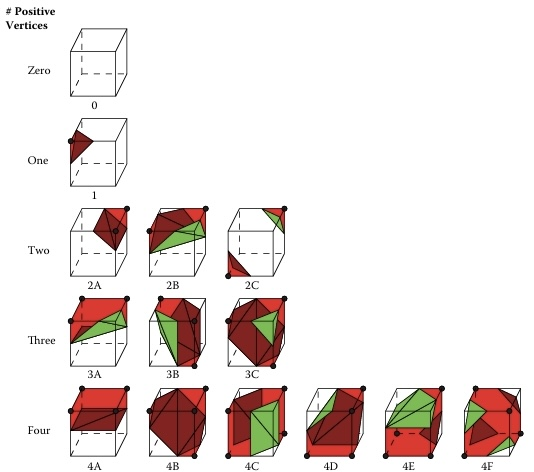
\includegraphics[width=\textwidth]{pictures/marching_cubes1.jpeg}
        \end{subfigure}
    \hspace{0.03\textwidth}
        \begin{subfigure}{0.35\textwidth}
        \centering
        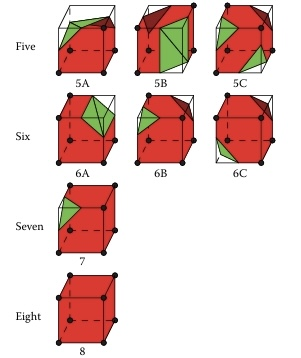
\includegraphics[width=\textwidth]{pictures/marching_cubes2.jpeg}
        \end{subfigure}
    \caption[Cube configurations]{Positive red regions contain positive black vertices and represent areas where the scalar value is above the isovalue. Green surfaces indicate the visible portion of the extracted isosurface, while dark red surfaces represent parts of the isosurface that are hidde behind the positive red regions in the 3D view (image retrieved from \cite{wenger2013}).}
\label{fig:marching_cubes}
\end{figure}

\subsection{Edge Interpolation}

Once the intersected edges of a voxel are identified through cell classification, the algorithm determines the precise coordinates where the isosurface crosses the grid. Because the scalar field is only sampled at discrete vertices, the exact intersection point must be approximated. Following the principles of piecewise-linear continuation, the Marching Cubes algorithm assumes that the scalar field $f$ varies linearly along each edge of the cube.

If the scalar values at two adjacent vertices $v_a$ and $v_b$ lie on opposite sides of the isovalue $c$, there exists at least one point $\mathbf{p}$ on the segment $v_a v_b$ such that $f(\mathbf{p}) = c$.

\begin{definition}%[Edge Intersection Point]
\label{def:edge-interp}
For an edge connecting vertices $v_a$ and $v_b$, with associated scalar values $s_a$ and $s_b$ and isovalue $\sigma$, the point $\mathbf{p}$ is defined as:
\begin{equation}
p = (1 - \alpha) v_a + \alpha v_b, \quad \text{where} \quad \alpha = \frac{\sigma - s_a}{s_b - s_a}.
\end{equation}
The parameter $\alpha \in [0, 1]$ represents the normalized distance along the edge. This linear approximation is computationally efficient and ensures that the reconstructed mesh remains continuous across adjacent voxels.
\end{definition}

The mathematical validity of this interpolation depends on the structural stability of the scalar field near the edge. If the gradient $\nabla f$ is non-zero (a regular point), the surface is locally a differentiable manifold, and the linear approximation provides a first-order accurate reconstruction. Near a singular point this assumption fails. On an edge with a sign change the denominator $s_b - s_a$ cannot vanish, since $|s_b-s_a|=|s_a|+|s_b|$, but both values are small because the gradient is close to zero, so their relative rounding errors are large, and the field along the edge is far from linear because the higher-order terms dominate. The interpolated vertex position is therefore unreliable. This is precisely the kind of sensitivity to small perturbations used in Unfolding, a singular point in the scalar field sits on the boundary of a bifurcation set, so an arbitrarily small change in the sampled values can push the local configuration across it, producing a qualitatively different (and possibly incorrect) triangulation. Such regions therefore typically require higher-order interpolation or adaptive refinement to recover the correct local topology \cite{frisken2000adaptively}.

\subsection{Ambiguities and Topological Inconsistencies}

A well-known limitation of the original Marching Cubes algorithm is that the same cube configuration can yield multiple valid triangulations. For instance, a face with alternating inside/outside vertices admits two valid diagonal connections, and choosing the wrong one may result in a non-manifold surface. This happens because the triangulation is determined locally within each cell without any consistency check against adjacent cells (see Figure~\ref{fig:ambiguity_comparison}).

%Dürst first identified such topological inconsistencies and showed that naive triangulation may violate surface continuity constraints \cite{durst1988marching}. To resolve such ambiguities, Nielson and Hamann proposed the \emph{Asymptotic Decider}, which uses bilinear interpolation over cube faces to consistently determine topology \cite{nielson1991asymptotic}.

\begin{figure}[!h]
    \centering
    \begin{subfigure}{0.48\textwidth}
        \centering
        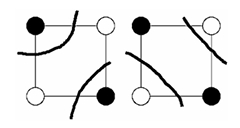
\includegraphics[width=\textwidth]{pictures/ambiguity.jpeg}
        \caption{Ambiguous face configuration (image retrieved from \cite{brentzen2012})}
        \label{fig:ambiguity2}
    \end{subfigure}
    \hfill
    \begin{subfigure}{0.48\textwidth}
        \centering
        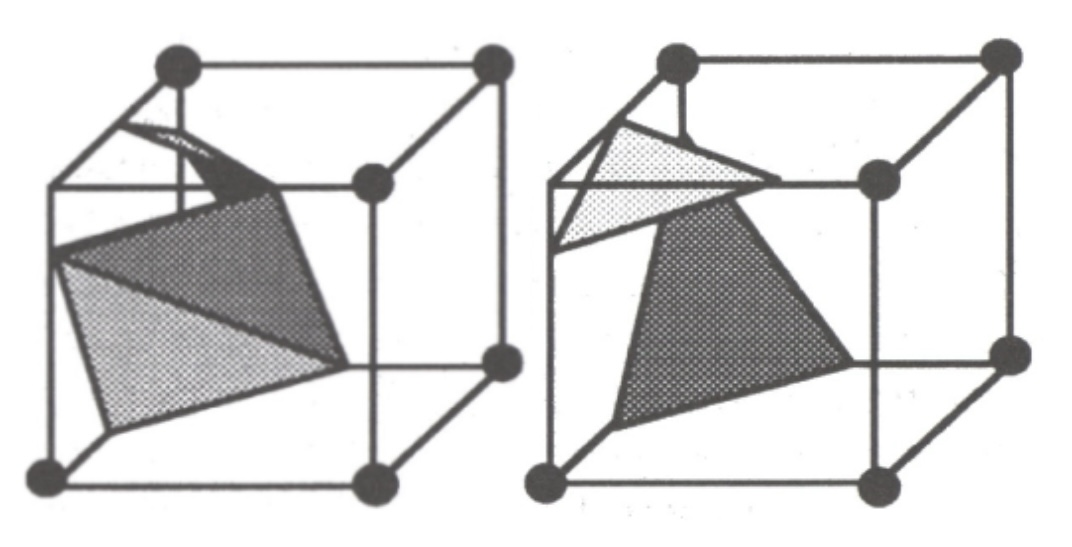
\includegraphics[width=\textwidth]{pictures/ambiguity3.jpeg}
        \caption{Two possible triangulations that yield a topologically correct isovalue surface (image retrieved from \cite{nielson1991asymptotic}).}
        \label{fig:ambiguity3}
    \end{subfigure}
    \caption{Comparison of ambiguities in 2D and 3D.}
    \label{fig:ambiguity_comparison}
\end{figure}

\begin{comment}
\begin{definition}
    \textbf{(Asymptotic Decider)}
Given bilinearly interpolated scalar values on a cube face, the decision of how to
connect edges is based on evaluating the saddle point of the interpolation function.
\end{definition}

Chernyaev further extended the algorithm with \emph{Marching Cubes 33}, which introduces
a more complete case table and resolves remaining ambiguities by refining cube
subdivision rules \cite{chernyaev1995marching}.

\subsection{Topological Correctness Improvements}

Lewiner et al.\ later proposed an efficient reformulation of Marching Cubes that
guarantees consistent topology by systematically resolving ambiguous cases
\cite{lewiner2003efficient}.

\begin{theorem}
    \textbf{(Topological Consistency Guarantee)}
Under the refined case classification scheme of Lewiner et al., the resulting mesh is
guaranteed to be free of cracks and topological inconsistencies for regular scalar
fields.
\end{theorem}

Despite these improvements, Marching Cubes can still fail near singular points where the
gradient is undefined or highly unstable: small perturbations in vertex values can lead
to different triangulations, causing visual artifacts or incorrect topology, especially
where the scalar field changes rapidly or is poorly sampled
\cite{lorensen1998marching,lewiner2003efficient}. Marching Cubes nonetheless remains
foundational; the Asymptotic Decider and Marching Cubes 33 significantly improve its
robustness and topological guarantees
\cite{lorensen1998marching,nielson1991asymptotic,chernyaev1995mc33,lewiner2003mc}.
\end{comment}

\section{Marching Tetrahedra}

The ambiguity issues in Marching Cubes are directly related to the hexahedral nature of the grid cells of this algorithm, which allows for several possible triangulations in certain configurations. The Marching Tetrahedra algorithms eliminates such ambiguities.

A voxel is split into a set of disjoint tetrahedra, each consisting of four vertices selected among the eight cube vertices, thereby partitioning the original cell into tetrahedra. For a tetrahedron $t$ with vertices $v_0, v_1, v_2, v_3$ and scalar values $s_i$, an isosurface is extracted by linearly interpolating along edges where the scalar function crosses zero relative to an iso-value $c$.

Since a tetrahedron has only four vertices, the amount of the possible sign configurations becomes much smaller as compared to the 256 cases in Marching Cubes. Each tetrahedron can be triangulated using one of the at most 16 possible sign configurations (see Figure~\ref{fig:marching_tetrahedra}).

\begin{figure}[!h]
    \centering
    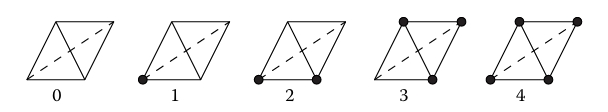
\includegraphics[width=0.8\textwidth]{pictures/marching_tetrahedra.jpeg}
    \caption[Tetrahedra configurations]{Tetrahedra configurations (image retrieved from \cite{wenger2013})} 
    \label{fig:marching_tetrahedra}
\end{figure} 

The intersection points of the edges of a tetrahedron are found using the same interpolation formula from Definition~\ref{def:edge-interp}, now applied to the edges of a tetrahedron instead of the cube edges.


Marching Tetrahedra guarantees that no face ambiguity occurs within a single simplex, ensuring locally consistent topology under correct interpolation assumptions. In other words, this method does not produce face-based ambiguity issues, like those seen in Marching Cubes. The drawback of this is that tetrahedral techniques sacrifice geometric efficiency for topological robustness. In Marching Cubes, one cube may create up to 5 triangles in each case, whereas its tetrahedral decomposition results in creation of a larger number of triangles because of multiple simplex interpolations, but all these tetrahedrons ensure creation of consistent triangulations \cite{nielson2008dual}.

Despite this robustness, the increased number of generated primitives can lead to generation of denser meshes in comparison with Marching Cubes, and inconsistent global triangulation may still happen if neighboring cubes use different subdivision schemes. Overall, Marching Tetrahedra sacrifices geometric simplicity for the sake of topological robustness in ambiguous and numerically difficult situations.

\section{Dual Contouring}

In both Marching Cubes and Marching Tetrahedra algorithms, the surface vertices lie along the grid edges and are determined through interpolation, which fails to represent sharp geometric features like edges or corners due to the nature of interpolation smoothing. The method introduced by Ju et al. \cite{ju2002dual} named Dual Contouring deals with this issue by changing the process to optimization-based placement of the surface vertices, meaning that the surface vertex is placed not on the grid edge, but inside the cell where the gradient field of the scalar field changes sign, using the geometric energy minimization function based on the local geometry of the surface.

For the regular voxel grid, the dual grid has one vertex per grid cell, not one per grid corner; each dual vertex corresponds to a local approximation of the isosurface in the corresponding cell. The data used to position each dual vertex is captured by Hermite data.

\begin{definition}
    \textbf{Hermite Data} is a set of samples associated with grid edges where the isosurface is intersected, consisting of intersection points $\mathbf{p}_i$, surface normals $\mathbf{n}_i$, and optionally gradient estimates of the scalar field.
\end{definition}

These values provide both positional and differential information crucial for accurate reconstruction. The edge intersection points themselves are computed using the same linear interpolation formula as in Marching Cubes (Definition~\ref{def:edge-interp}), but unlike Marching Cubes, Dual Contouring does not place vertices directly at these points; instead, it uses them as constraints in an optimization problem.

\subsection{Quadratic Error Function (QEF)}

The optimization problem to find the position of each dual vertex is based on the Quadratic Error Function that computes the point in the cell that best satisfies all local tangent plane constraints simultaneously.

\begin{definition}
\textbf{(QEF)}
Given Hermite constraints $(\mathbf{p}_i, \mathbf{n}_i)$, the QEF is
\[
E(\mathbf{x}) = \sum_i \left( \mathbf{n}_i \cdot (\mathbf{x} - \mathbf{p}_i) \right)^2.
\]
\end{definition}

The optimal position of the vertex $\mathbf{x}^* = \arg\min_{\mathbf{x}} E(\mathbf{x})$. The solution $\mathbf{x}^*$ to the QEF minimizes the squared distance to all tangent planes defined by Hermite data. The least-square formulation enables a stable and efficient computation of vertex positions with geometric details \cite{ju2002dual}.  

One of the most important advantages of the Dual Contouring algorithm is its ability to preserve sharp edges and corners, while the Marching Cubes algorithm interpolates these features. Feature-sensitive reconstruction requires explicit handling of discontinuities in the surface normal field, achieved by incorporating Hermite constraints directly into vertex positioning \cite{kobbelt2001feature}.

In regions where Hermite constraints are sparse or poorly conditioned, for instance, when normals are nearly parallel or intersection points nearly collinear, the QEF may become ill-defined. In order to achieve stability in such degenerate cases, it is essential to use regularization techniques like positional constraints or clamping solution \cite{ju2002dual}.  Modern extensions to adaptive grids allow higher resolution only where needed.  Adaptive dual contouring leads to substantial memory savings without compromising on sharp feature retention.

With precise Hermite data, the vertices obtained through QEF minimization will lie very close to the isosurface along with retaining the first order geometry of edges and corners. Dual Contouring technique thus evolves from interpolation based surface extraction to optimization based surface reconstruction technique utilizing Hermite data, enabling superior feature preservation and more flexible topology handling \cite{ju2002dual,kobbelt2001feature}.

\section{Differential Properties in Polygonization}
\begin{comment}
Polygonal isosurface extraction methods aim not only to reconstruct geometry but also to
approximate the differential properties of the underlying implicit surface, namely
surface normals, curvature, and geometric error, all essential for visual fidelity and
numerical correctness.

\begin{definition}
    \textbf{(Surface Normals on Polygonal Meshes)}
Given a triangle mesh $\mathcal{M}$ approximating an isosurface, the normal vector at a
vertex is typically a weighted average of adjacent face normals,
\[
\mathbf{n}_v = \frac{\sum_{f \in \mathcal{N}(v)} w_f \mathbf{n}_f}{\left\|\sum_{f \in
\mathcal{N}(v)} w_f \mathbf{n}_f \right\|},
\]
where $\mathcal{N}(v)$ is the set of adjacent faces and $w_f$ a weighting factor based on
area or angle.
\end{definition}

Rusinkiewicz shows that such averaging schemes give robust normal estimates on discrete
meshes, especially combined with local neighborhood analysis
\cite{rusinkiewicz2004estimating}. Beyond normals, the second-order geometry of the
surface is captured by curvature.

\begin{definition}
    \textbf{(Curvature on Triangle Meshes)}
Curvature describes how a surface deviates from being planar; for a polyhedral surface
it is approximated using discrete differential operators applied to vertex
neighborhoods.
\end{definition}

Taubin introduces a tensor-based formulation of curvature estimation on polygonal
meshes, derived from local variations of normals \cite{taubin1995estimating}.

\begin{theorem}
    \textbf{(Discrete Curvature Approximation)}
Let $\mathcal{M}$ be a sufficiently dense triangulation of a smooth surface. Then the
discrete curvature tensor converges to the continuous curvature tensor as the mesh
resolution increases.
\end{theorem}

\textit{Proof sketch.} Convergence follows from the consistency of local surface
approximations and the stability of weighted normal averaging in shrinking neighborhoods
\cite{taubin1995estimating}.

\subsection{Curvature-Sensitive Reconstruction}

Regions of high curvature typically require finer sampling to preserve geometric detail,
while flatter regions can be approximated with fewer primitives; Rusinkiewicz
demonstrates that curvature estimation can also improve smoothing, remeshing, and feature
detection \cite{rusinkiewicz2004estimating}. Beyond curvature, it is also important to
quantify how closely a polygonal mesh approximates the original surface.

\begin{definition}
    \textbf{(Geometric Error Metrics)}
Let $\mathcal{S}$ be the original implicit surface and $\mathcal{M}$ its polygonal
approximation. The geometric error at $\mathbf{x} \in \mathcal{M}$ is the Euclidean
distance to the closest point on $\mathcal{S}$,
\[
E(\mathbf{x}) = \min_{\mathbf{y} \in \mathcal{S}} \|\mathbf{x} - \mathbf{y}\|.
\]
\end{definition}

Cignoni et al.\ formalize this notion in the Metro framework for measuring deviation
between meshes and reference surfaces \cite{cignoni1998metro}.

\begin{theorem}
    \textbf{(Error Accumulation in Polygonization)}
Let $\mathcal{M}_h$ be a mesh generated with resolution parameter $h$. Then the
geometric error satisfies $E(\mathcal{M}_h) = \mathcal{O}(h)$ under uniform sampling
assumptions.
\end{theorem}

This follows from the relationship between sampling density and approximation accuracy
in surface reconstruction \cite{cignoni1998metro}.

\subsection{Relation to Quadric Error Metrics}

Garland and Heckbert introduced quadric error metrics for measuring and minimizing
geometric deviation during surface simplification; although designed for decimation, the
same quadratic-error idea is closely related to error control in reconstruction.

\begin{definition}
    \textbf{(Quadric Error Metric)}
Each vertex is associated with a quadratic form representing the squared distance to a
set of planes, whose optimal position minimizes $E(\mathbf{x}) = \mathbf{x}^T Q
\mathbf{x}$, where $Q$ is the accumulated error matrix.
\end{definition}

This formulation provides a computationally efficient way to approximate geometric
deviation \cite{garland1997surface}. Beyond geometric accuracy, the topology of the
reconstructed surface must also be correct: it must preserve the right connectivity and
avoid artificial holes or self-intersections. Edelsbrunner and Mücke introduced
$\alpha$-shapes as a formal framework for defining the topology of a point set based on a
scale parameter $\alpha$ \cite{edelsbrunner1994three}.

\begin{theorem}
    \textbf{(Topological Consistency of Alpha Shapes)}
For a sufficiently dense sampling of a compact surface, the $\alpha$-shape converges to
the correct topological structure of the original object for an appropriate choice of
$\alpha$.
\end{theorem}

If a surface is under-sampled in regions of high curvature, however, polygonization may
introduce spurious handles or disconnected components, which alpha-shape theory explains
as incorrect scale selection \cite{edelsbrunner1994three}.

Taken together, normals, curvature, and geometric error provide the essential feedback
for evaluating and improving polygonal isosurface reconstruction, connecting discrete
mesh representations back to the underlying smooth geometry with which this chapter began
\cite{rusinkiewicz2004estimating,taubin1995curvature,cignoni1998metro,garland1997quadric,edelsbrunner1994three}.
\end{comment}

\label{sec:poly-quality}

The extraction methods of this chapter produce a triangle mesh that should approximate the implicit surface. To compare different methods, and as the thesis assignment requires, to judge their geometric accuracy and topological correctness, we need to say precisely what a good approximation is. This section collects the notions used for that: normals, the distance between a mesh and a surface, and simple topological invariants of a mesh. At the end we look at what happens to these quantities near a singular point.

\subsection{Normals of the Extracted Mesh}

For an implicit surface the normal is known exactly at every regular point: by the theorem on the surface normal in Chapter~\ref{ch:implicit} it is $\nabla f/\|\nabla f\|$. Marching Cubes implementations therefore usually assign to every mesh vertex the normalized gradient at that vertex \cite{lorensen1998marching,bloomenthal1997introduction}. Another option, which uses only the mesh, is to average the normals of the triangles around a vertex, weighted by their areas or angles \cite{Botsch}. Near a regular point both give almost the same result. Near a singular point the gradient is small and changes direction quickly, so normalizing it divides a small and inexact vector by its small length; the computed normal is then unreliable and neighbouring vertices can get very different normals. Normals are not used in our evaluation for this reason, but this instability returns in Chapter~\ref{ch:method}, where we try to follow the gradient direction near the singular point.

\subsection{Geometric Accuracy}

The geometric error of a mesh is the distance between the mesh and the surface it approximates. The standard way to measure it is the Hausdorff distance, used for example in the Metro tool for comparing meshes \cite{cignoni1998metro}.

\begin{definition}
\label{def:hausdorff}
For a point $p$ and a closed set $B\subset\mathbb{R}^3$ let $\operatorname{dist}(p,B)=\inf_{q\in B}\|p-q\|$. The \emph{one-sided distance} from a closed set $A$ to $B$ is $\sup_{p\in A}\operatorname{dist}(p,B)$, and the \emph{Hausdorff distance} of $A$ and $B$ is
\[
d_H(A,B)=\max\Big\{\sup_{p\in A}\operatorname{dist}(p,B),\ \sup_{p\in B}\operatorname{dist}(p,A)\Big\}
\]
\cite{rockafellar1998variational}.
\end{definition}

The two one-sided distances measure different things. The distance from the mesh to the surface is small if every point of the mesh lies close to the surface. The distance from the surface to the mesh is small if every part of the surface is represented by some part of the mesh. A mesh that misses a part of the surface completely can still have all its vertices on the surface, and only the second one-sided distance reveals this. For this reason we always measure both directions. In Chapter~\ref{ch:theory} we use a local version of this distance, restricted to a box around the singular point (Definition~\ref{def:local-hausdorff}).

\subsection{Topological Correctness}

A mesh can be close to the surface and still have the wrong topology, for example two pieces where there should be one. We describe the topology of a mesh by a few simple quantities \cite{Botsch,edelsbrunner2010computational}.

\begin{definition}
\label{def:mesh-topology}
Let $\mathcal{M}$ be a triangle mesh with $V$ vertices, $E$ edges and $F$ triangles. An edge is a \emph{boundary edge} if it belongs to exactly one triangle and a \emph{non-manifold edge} if it belongs to more than two triangles. The \emph{Euler characteristic} of $\mathcal{M}$ is
\[
\chi(\mathcal{M})=V-E+F .
\]
\end{definition}

\begin{theorem}[\cite{hatcher2002algebraic,edelsbrunner2010computational}]
\label{thm:euler}
The Euler characteristic depends only on the topology of the mesh: homeomorphic meshes have the same $\chi$. A compact connected orientable surface of genus $g$ with $b$ boundary curves has $\chi=2-2g-b$.
\end{theorem}

For example a disk has $\chi=1$, an annulus $\chi=0$ and a sphere $\chi=2$. The Euler characteristic adds over connected components, so two separate disks have $\chi=2$, while two disks that meet in one point (which is not a surface any more, but still a triangle mesh) have $\chi=1+1-1=1$. Together with Corollary~\ref{cor:cone-topology} this gives a simple test: near an isolated singular point, a correct mesh is connected and has $\chi=1$. The test is not complete, since different surfaces can have the same $\chi$, but it detects exactly the failures that occur at singular points: pieces that should meet at the singular point but do not. In addition we count boundary edges that are not caused by cutting the mesh with a box (holes) and non-manifold edges.

\subsection{Behaviour Near Singular Points}

The extraction methods of this chapter were designed for regular surfaces, and near a singular point their assumptions fail in a few concrete ways. The first one is a direct consequence of the construction of Marching Cubes.

\begin{proposition}
\label{prop:mc-vertices}
Every vertex of a Marching Cubes mesh lies on an edge of the voxel grid whose endpoints have values on different sides of the iso-value, or at a grid node with a value equal to the iso-value. In particular, a singular point that lies on no grid edge is never a vertex of the mesh.
\end{proposition}

\begin{proof}
Marching Cubes creates vertices only by the edge interpolation of Definition~\ref{def:edge-interp}, which is applied to edges with a sign change and gives a point of the segment $v_av_b$; for $\alpha\in\{0,1\}$ this point is an endpoint.
\end{proof}

So the mesh can pass near a singular point but triangulates the cells around it as if the surface were smooth there. The second failure concerns thin features. If all eight corners of a cell have the same sign, Marching Cubes produces no triangle in that cell, even if a part of the surface thinner than a cell passes through it. Near a singular point such thin parts are typical, since the surface can narrow down to a tip, as for the horn $x^2+y^2+z^3$. The third failure concerns topology. The Asymptotic Decider \cite{nielson1991asymptotic}, Marching Cubes 33 \cite{chernyaev1995marching} and its implementation with topological guarantees \cite{lewiner2003efficient} resolve the ambiguous configurations of Section~\ref{sec:marching-cubes} so that the mesh has the topology of the trilinear interpolant in every cell. Near a singular point the trilinear interpolant itself can have a different topology than the surface, for example two nappes of a cone that do not touch, and no choice of triangulation can repair this. Methods with stronger guarantees, such as the isotopic approximation of Plantinga and Vegter \cite{plantinga2004isotopic}, assume that the surface has no singular points at all, and the method of Stander and Hart \cite{stander1997guaranteeing} tracks the critical points of $f$ to guarantee the topology of the polygonization, building on Morse theory, which works with non-degenerate critical points. A survey of polygonization methods for implicit surfaces can be found in \cite{araujo2015survey}. A method that represents the neighbourhood of a singular point faithfully therefore has to use additional knowledge about the singularity. Chapter~\ref{ch:theory} develops this knowledge, and Chapter~\ref{ch:method} uses it.


% =============================================================================
\chapter{Perturbations of Isolated Singularities}
\label{ch:theory}
% =============================================================================

Section~\ref{sec:singularities} described the singular points of an implicit surface, and Chapter~\ref{ch:extraction} showed that these are exactly the places where voxel methods like Marching Cubes become unreliable. One way to understand a singular point better is to disturb it a little and look at what the disturbance does, which is the idea of unfolding from Section~\ref{sec:unfolding}. In this chapter we apply this idea to implicit surfaces. We consider
\[
H_k=F+kG,\qquad S_k=\{p\in\mathbb{R}^3 \mid H_k(p)=0\},
\]
where $F$ has an isolated singular point at the origin $P$ and $G$ is a fixed polynomial. For $k=0$ we get the singular surface $S_0$, for small $k\neq0$ a nearby surface. We ask:
\begin{enumerate}
    \item[(Q1)] How fast does $S_k$ approach $S_0$ near $P$ as $k\to0$?
    \item[(Q2)] What happens to $P$: does it stay on the surface, does it stay singular? Are new singular points created, how many, of which type, and how fast do they approach $P$?
    \item[(Q3)] How much of this does a uniform voxel grid show?
\end{enumerate}
The two signs of $k$ are treated separately, because $k<0$ and $k>0$ can behave quite differently. The chapter is theoretical. Results from the literature are quoted with their source, and the statements derived for this thesis are proved. The numerical methods that compute the quantities defined here are described in Chapter~\ref{ch:method}, and the measurements are reported in Chapter~\ref{ch:experiments}.

% -----------------------------------------------------------------------------
\section{One-Parameter Families of Implicit Surfaces}
\label{sec:families}

\begin{definition}
\label{def:family}
Let $F,G:\mathbb{R}^3\to\mathbb{R}$ be polynomials. The \emph{one-parameter family} defined by $F$ and $G$ consists of the functions and surfaces
\begin{equation}
\label{eq:family}
H_k=F+kG,\qquad S_k=\{p\in\mathbb{R}^3 \mid H_k(p)=0\},\qquad k\in\mathbb{R}.
\end{equation}
We call $S_0=\{F=0\}$ the \emph{singular surface}, $G$ the \emph{perturbation} and $k$ the \emph{parameter} of the family.
\end{definition}

We always assume that $S_0$ has an isolated singular point $P$ (Definition~\ref{def:isolated}) and, after a translation, that $P$ is the origin. All statements are local: they concern the part of $S_k$ near $P$, for small $|k|$. We measure local quantities in the closed box
\begin{equation}
\label{eq:box}
Q_a=\{p\in\mathbb{R}^3 \mid \|p\|_\infty\le a\}=[-a,a]^3,\qquad
\|p\|_\infty=\max\{|p_1|,|p_2|,|p_3|\}.
\end{equation}
A box is used instead of a ball because it is aligned with the voxel grid of Chapter~\ref{ch:extraction}. Nothing in this chapter depends on this choice: since $\|p\|_\infty\le\|p\|_2\le\sqrt3\,\|p\|_\infty$, every box contains a ball and is contained in a ball of comparable size, so limits and rates of convergence are the same for boxes and balls, and only constants change.

\begin{definition}
\label{def:stationary}
A point $q$ is a \emph{stationary point} of $H_k$ if $\nabla H_k(q)=0$. It is a \emph{singular point of the surface} $S_k$ if, in addition, $H_k(q)=0$.
\end{definition}

The distinction matters throughout. A perturbation typically creates several stationary points near $P$, but only those on the zero level are singular points of the surface; a stationary point with $H_k(q)\neq0$ does not lie on $S_k$ at all.

The first part of question (Q2), what happens at the point $P$ itself, can be answered without any computation. Because $F(P)=0$ and $\nabla F(P)=0$,
\begin{equation}
\label{eq:at-origin}
H_k(P)=k\,G(P),\qquad \nabla H_k(P)=k\,\nabla G(P),\qquad
\operatorname{Hess}H_k(P)=\operatorname{Hess}F(P)+k\operatorname{Hess}G(P).
\end{equation}

\begin{proposition}
\label{prop:fate}
Let $k\neq0$.
\begin{enumerate}
    \item If $G(P)\neq0$, then $P\notin S_k$: the surface \emph{leaves} $P$.
    \item If $G(P)=0$ and $\nabla G(P)\neq0$, then $P$ is a \emph{regular} point of $S_k$.
    \item If $G(P)=0$ and $\nabla G(P)=0$, then $P$ \emph{stays singular}.
\end{enumerate}
\end{proposition}

\begin{proof}
All three statements follow from \eqref{eq:at-origin} and Definition~\ref{def:regular-singular}.
\end{proof}

In the third case the type of the singular point is decided by the Hessian and the higher terms. How degenerate it is can be read from the \emph{corank} of $P$, the number of zero eigenvalues of $\operatorname{Hess}H_k(P)$. Corank $0$ means that the Hessian is invertible, so by the Morse lemma (Theorem~\ref{thm:morse}) $P$ is an ordinary double point $A_1$; a larger corank means a more degenerate point. For example $x^3+y^3+z^3+kx^2$ has the leading terms $kx^2+y^3+z^3$, the normal form of $D_4$: the singular point persists but becomes simpler, with $\mu=4$ instead of $8$. Proposition~\ref{prop:fate} says nothing about singular points away from $P$; those are the subject of Sections~\ref{sec:conservation} and~\ref{sec:diagonal}.

\begin{definition}
\label{def:order}
Write $G=G_0+G_1+G_2+\cdots$, with $G_j$ homogeneous of degree $j$. The \emph{order} of $G$ at $P$ is the smallest $m$ with $G_m\neq0$.
\end{definition}

The order is local and does not have to equal the degree: $G=x^2+x$ has degree two but order one. In terms of the order, Proposition~\ref{prop:fate} reads: $m=0$ means that $P$ leaves the surface, $m=1$ that $P$ becomes regular, and $m\ge2$ that $P$ stays singular.

% -----------------------------------------------------------------------------
\section{Measuring How Far Two Surfaces Are}
\label{sec:convergence}

We compare $S_k$ with $S_0$ inside the box $Q_a$ around $P$.

\begin{definition}
\label{def:local-hausdorff}
For closed sets $A,B\subset\mathbb{R}^3$ the \emph{local Hausdorff distance} in the box $Q_a$ is
\[
d_a(A,B)=\max\Big\{\sup_{p\in A\cap Q_a}\operatorname{dist}(p,B),\ \sup_{p\in B\cap Q_a}\operatorname{dist}(p,A)\Big\},
\]
with the convention $\sup\emptyset=0$. We write $d(k)=d_a(S_k,S_0)$.
\end{definition}

In words: take every point of one surface inside the box, find how far it is from the other surface, and take the worst case, in both directions. If $d(k)$ is small, every part of each surface near $P$ is close to the other surface. The points are taken inside the box, but their distance is measured to the whole other surface, so the parts of the other surface just outside the box are not counted as errors. For $a=\infty$ this is the Hausdorff distance of Definition~\ref{def:hausdorff}.

To describe how fast quantities go to zero we use the usual asymptotic notation.

\begin{definition}
\label{def:bigO}
Let $\beta\ge0$. We write $f(k)=O(|k|^\beta)$ (``$f$ is of order $|k|^\beta$'') if there are constants $C>0$ and $k_0>0$ with $|f(k)|\le C|k|^\beta$ for $0<|k|<k_0$, and $f(k)=\Theta(|k|^\beta)$ if moreover $|f(k)|\ge c|k|^\beta$ for some $c>0$.
\end{definition}

For example, ``the surface moves by $O(|k|)$'' means that it moves by a distance at most proportional to $|k|$.

\begin{definition}
\label{def:rate}
Let $k\to0$ from one side. The surface $S_k$ converges to $S_0$ with \emph{rate} $\alpha>0$ if $d(k)=\Theta(|k|^\alpha)$; we then write
\[
d(k)\approx C\,|k|^\alpha\qquad\text{for small }|k|,
\]
and call $C$ the \emph{constant}. Similarly, singular points $q(k)$ of $S_k$ converge to $P$ with rate $\gamma$ if $\|q(k)\|=\Theta(|k|^\gamma)$.
\end{definition}

A larger $\alpha$ means faster convergence. The rate $\alpha=1$ means that the surface moves proportionally to $k$; $\alpha=\tfrac13$ means that it moves much more, since $|k|^{1/3}\gg|k|$ for small $k$ (for $k=10^{-3}$: $0.1$ against $0.001$). The constant $C$ tells how large the deformation is, not how fast it shrinks. On a log--log plot, where both axes use logarithmic scales, $d(k)\approx C|k|^\alpha$ becomes the straight line $\log d=\log C+\alpha\log|k|$ with slope $\alpha$, which is how the rate is measured in Chapter~\ref{ch:experiments}.

Some facts about the convergence hold without computing anything. First, every limit of points $q_k\in S_k\cap Q_a$ lies on $S_0$, for every $G$: since $G$ is bounded on $Q_a$, $F(q_k)=-kG(q_k)\to0$. Second, if $F$ takes both signs in every neighbourhood of a point $p\in S_0$, then $S_k$ meets every neighbourhood of $p$ for small $|k|$. For the cubic cones of our experiments this gives the following statement.

\begin{proposition}
\label{prop:set-convergence}
Let $F$ be a homogeneous cubic with an isolated singular point at the origin. Then for every polynomial $G$ and every $a>0$ the surfaces $S_k$ converge to $S_0$ inside $Q_a$ in the sense of sets (Painlevé--Kuratowski convergence \cite{rockafellar1998variational}), from both sides of $k=0$.
\end{proposition}

\begin{proof}
Limits of points of $S_k\cap Q_a$ lie on $S_0$ by the first fact. For the second, let $p\in S_0$ and let $U$ be a convex neighbourhood of $p$. The gradient $\nabla F$ is homogeneous of degree two, so if it vanished at some $q\neq0$ it would vanish on the whole line through $q$, and the singular point would not be isolated. Hence every $p\neq0$ of $S_0$ is a regular point, and $F$ takes both signs in $U$. For $p=0$ choose $u$ with $F(u)\neq0$; then $F(tu)=t^3F(u)$ and $F(-tu)=-t^3F(u)$ have opposite signs, and both points lie in $U$ for small $t>0$. In both cases there are $a',b'\in U$ with $F(a')<0<F(b')$. For $|k|$ small enough $H_k$ keeps these signs, and by the intermediate value theorem it vanishes on the segment $[a',b']\subset U$. Hence $S_k\cap U\neq\emptyset$.
\end{proof}

Set convergence can fail where $F$ does not change sign. For $x^2+y^2+z^2+k$ the surface is empty for $k>0$ and a sphere of radius $\sqrt{|k|}$ for $k<0$, so the convergence is only one-sided.

An upper bound on the distance follows from the Łojasiewicz inequality.

\begin{theorem}[Łojasiewicz inequality \cite{lojasiewicz1959division,bochnak1998real}]
\label{thm:lojasiewicz}
Let $F$ be a polynomial and $K\subset\mathbb{R}^3$ compact. There are constants $c>0$ and $\ell\ge1$ such that $|F(p)|\ge c\operatorname{dist}(p,S_0)^\ell$ for all $p\in K$.
\end{theorem}

On $S_k$ we have $|F|=|k||G|$, so no point of $S_k\cap K$ is farther than $(|k|\max_K|G|/c)^{1/\ell}$ from $S_0$: one half of the local Hausdorff distance is always $O(|k|^{1/\ell})$. For a homogeneous cubic with $\nabla F\neq0$ away from the origin one can take $\ell=3$. On the unit sphere $F$ vanishes only to first order at its zeros, so $|F(u)|\ge c\operatorname{dist}(u,S_0)\ge c\operatorname{dist}(u,S_0)^3$ there, and both sides scale by $t^3$ under $u\mapsto tu$ because $S_0$ is a cone. The precise rate is given by the scaling argument of the next section.

% -----------------------------------------------------------------------------
\section{Scaling Estimate for the Convergence Rate}
\label{sec:scaling}
\label{sec:r-scaling}

\subsection{The Idea in One Variable}

Consider $f_k(x)=x^3+kx$. For $k=0$ its only zero is $x=0$, a triple zero. For $k<0$ there are three zeros, $0$ and $\pm\sqrt{-k}$; for $k>0$ only $0$ remains, but the graph turns from a horizontal inflection into a steep crossing (Figure~\ref{fig:one-variable}). Both changes happen at the same length scale $|x|\approx\sqrt{|k|}$, which can be predicted without solving anything: the two terms $x^3$ and $kx$ are of equal size when $|x|^3=|k|\,|x|$, that is, $|x|=|k|^{1/2}$. For $|x|\gg|k|^{1/2}$ the cubic term dominates and $f_k$ looks like $f_0$, for $|x|\ll|k|^{1/2}$ the perturbation dominates. The same balance for $f_k(x)=x^3+k$ gives $|x|^3=|k|$, the scale $|k|^{1/3}$, and indeed the zero is $x=-k^{1/3}$.

\begin{figure}[!h]
\centering
\begin{tikzpicture}
\begin{axis}[width=0.62\textwidth, height=0.42\textwidth,
    xlabel={$x$}, ylabel={$f_k(x)$}, xmin=-0.32, xmax=0.32, ymin=-0.012, ymax=0.012,
    axis lines=middle, legend pos=north west, legend cell align=left,
    legend style={font=\small}, yticklabel style={/pgf/number format/fixed}]
\addplot[black, thick, domain=-0.3:0.3, samples=120] {x^3};
\addlegendentry{$k=0$}
\addplot[blue, thick, domain=-0.3:0.3, samples=120] {x^3-0.01*x};
\addlegendentry{$k=-0.01$}
\addplot[red, thick, dashed, domain=-0.3:0.3, samples=120] {x^3+0.01*x};
\addlegendentry{$k=+0.01$}
\addplot[gray, densely dotted] coordinates {(-0.1,-0.012) (-0.1,0.012)};
\addplot[gray, densely dotted] coordinates {(0.1,-0.012) (0.1,0.012)};
\end{axis}
\end{tikzpicture}
\caption[Scaling in one variable]{$f_k(x)=x^3+kx$. The changes caused by the perturbation are confined to $|x|\lesssim\sqrt{|k|}=0.1$ (dotted lines); outside, the three graphs are almost the same.}
\label{fig:one-variable}
\end{figure}

\subsection{Weights and the Scaling Estimate}

For some surfaces the variables enter the equation with different powers. In $F=x^2+y^2+z^3$ the variables $x$ and $y$ appear in quadratic form, while $z$ appears in cubic form, so the balance has to be done with a different length in each direction. This is what the weights of Definition~\ref{def:quasihomogeneous} are for.

\begin{definition}
\label{def:principal-part}
Let $w=(w_x,w_y,w_z)$ be positive weights. The \emph{principal part} $F_0$ of $F$ is the sum of its terms of weighted degree $1$, provided all other terms have weighted degree larger than $1$. For a perturbation $G$, the \emph{weighted order} $d_w(G)$ is the minimum of $d_w(x^ay^bz^c)$ over the monomials $x^ay^bz^c$ of $G$.
\end{definition}

The principal parts and weights of the surfaces used in the experiments are listed below.
\begin{center}
\small
\begin{tabular}{l l}
\toprule
Principal part $F_0$ & Weights $w$ \\
\midrule
$x^2+y^2-z^2$ & $(\frac12,\frac12,\frac12)$ \\
$x^2\pm y^2+z^3$ & $(\frac12,\frac12,\frac13)$ \\
$x^2+y^3+z^2$ & $(\frac12,\frac13,\frac12)$ \\
$x^2+y^3+z^3$, $x^2+y^3-3yz^2$ & $(\frac12,\frac13,\frac13)$ \\
the four cubic cones & $(\frac13,\frac13,\frac13)$ \\
\bottomrule
\end{tabular}
\end{center}

On a region where the coordinates have the sizes $t^{w_x}$, $t^{w_y}$ and $t^{w_z}$, the principal part of $F$ has size approximately $t$, while the perturbation has size approximately $|k|\,t^{d_w(G)}$. Balancing these terms gives
\[
t=|k|\,t^{d_w(G)}
\quad\Longrightarrow\quad
t=\lambda(k):=|k|^{1/(1-d_w(G))}
\]
when $d_w(G)<1$. We call $\lambda(k)$ the \emph{characteristic scale} of the family. The deformation is concentrated in the \emph{inner region} around $P$, whose size along the axis $i$ is $\lambda(k)^{w_i}$; outside it, in the \emph{outer region}, $S_k$ stays close to $S_0$ and moves only by $O(|k|)$. This gives the following scaling estimate for the convergence rate:
\begin{equation}
\alpha\in
\left[
\min\left(1,\frac{w_{\min}}{1-d_w(G)}\right),\
\min\left(1,\frac{w_{\max}}{1-d_w(G)}\right)
\right],
\label{eq:r-alpha}
\end{equation}
where $w_{\min}$ and $w_{\max}$ are the smallest and the largest weight. If $d_w(G)\ge1$, the estimated rate is $\alpha=1$. This principle has its background in the theory of deformations of quasi-homogeneous singularities \cite{arnold1985singularities,greuel2007introduction}.

For example, for $F=x^2+y^2+z^3$ and $G=1$ we have $d_w(G)=0$, which gives the predicted range $\alpha\in[\frac13,\frac12]$. For $G=z$ we have $d_w(G)=\frac13$, which gives $\alpha\in[\frac12,\frac34]$. For the ordinary double point all weights are $\frac12$: $G=1$ gives $\alpha=\frac12$, and $G=x$, with $d_w(x)=\frac12$, gives $\alpha=1$, so a linear perturbation moves an ordinary double point linearly and does not open it at first order. For the cubic cones all weights are $\frac13$, and if the lowest terms of $G$ have the ordinary degree $m<3$ the estimate reduces to
\[
\alpha=\frac{1}{3-m}.
\]

These values are scaling estimates rather than guaranteed bounds. The exponent observed in the experiments also depends on the real geometry of the surface and on the sign of $k$, and the predicted ranges are therefore compared with the measured rates in Chapter~\ref{ch:experiments}. In one case the estimate is exact.

\begin{proposition}[Self-similarity]
\label{prop:self-similar}
Let $F$ be homogeneous of degree $d$ and $G$ homogeneous of degree $m<d$, let $k\neq0$, $\sigma=\operatorname{sign}k$ and $\lambda=|k|^{1/(d-m)}$. Then
\begin{enumerate}
    \item $S_k=\lambda M_\sigma$, where $M_\sigma=\{u \mid F(u)+\sigma G(u)=0\}$ is the \emph{model surface};
    \item $d_a(S_k,S_0)=\lambda\,d_{a/\lambda}(M_\sigma,S_0)$, and $d_a(S_k,S_0)/\lambda$ increases to the Hausdorff distance $C_\sigma=d_\infty(M_\sigma,S_0)$ as $k\to0$ with fixed sign $\sigma$.
\end{enumerate}
Consequently, if $0<C_\sigma<\infty$, then $d_a(k)=C_\sigma|k|^{1/(d-m)}(1+o(1))$, and the rate of convergence is exactly $\alpha=1/(d-m)$.
\end{proposition}

\begin{proof}
(1) $H_k(\lambda u)=\lambda^dF(u)+k\lambda^mG(u)=\lambda^d\big(F(u)+\sigma G(u)\big)$, because $k\lambda^m=\sigma\lambda^{d-m}\lambda^m$. (2) The cone satisfies $S_0=\lambda S_0$, and $\lambda Q_{a/\lambda}=Q_a$, so all points and distances in Definition~\ref{def:local-hausdorff} scale by $\lambda$. The box $Q_{a/\lambda}$ grows as $\lambda\to0$, and $d_b$ is nondecreasing in $b$, with the limit $d_\infty$.
\end{proof}

So for a homogeneous $G$ the family is exactly self-similar for each sign of $k$: $S_k$ is a fixed surface, scaled by $|k|^{1/(d-m)}$. The model surfaces for $k<0$ and $k>0$ are in general different, which is why the constants $C_-$ and $C_+$ can differ even when the rates agree. For the cubic cones the rate is exactly $\frac13$ for $G=1$, $\frac12$ for linear $G$ and $1$ for homogeneous quadratic $G$; the constant $C_\sigma$ depends on the direction of $G$, not only on its order.

\subsection{Relation to the Blowup}

The substitution $p=\lambda(k)u$ is the weighted blowup of Section~\ref{sec:blowup}, applied to the point $(p,k)=(0,0)$ of the four-dimensional space of positions and parameters, with the weight $1$ (or $w_i$) for the spatial variables and the weight $d-m$ (or $1-d_w(G)$) for $k$. The model surfaces $M_\pm$ are what is seen in the directional charts $\bar k=\pm1$ \cite{kristiansen2019resolution}. In this sense the blowup, introduced in Chapter~\ref{ch:implicit} for dynamical systems, resolves the singular limit $k\to0$ of a family of implicit surfaces: it separates the inner region, where the surface is a fixed model, from the outer region, where it is the singular surface.

% -----------------------------------------------------------------------------
\section{Essential and Inessential Perturbations}
\label{sec:essential}

The scaling explains the size of the deformation. It does not explain which perturbations really change the singularity. Some perturbations only move or stretch the surface without changing the local type of the singular point.

\begin{proposition}
\label{prop:first-order}
Let $G=a_x\partial_xF+a_y\partial_yF+a_z\partial_zF+bF$ with polynomials $a_x,a_y,a_z,b$, and let $a=(a_x,a_y,a_z)$. Then
\[
\big(1+k\,b(p)\big)\,F\big(p+k\,a(p)\big)=F(p)+kG(p)+O(k^2)
\]
uniformly for $p$ in a bounded set.
\end{proposition}

\begin{proof}
By Taylor's theorem, $F(p+ka(p))=F(p)+k\,a(p)\cdot\nabla F(p)+O(k^2)$. Multiplying by $1+kb(p)$ gives $F+k\big(a\cdot\nabla F+bF\big)+O(k^2)=F+kG+O(k^2)$.
\end{proof}

Near $P$ the factor $1+kb$ is close to $1$ and does not change the zero set, and $p\mapsto p+ka(p)$ is a small change of coordinates. So, to first order in $k$, adding $kG$ is equivalent to a change of coordinates and a multiplication of the equation by a factor close to $1$: the singularity is only moved or stretched, not genuinely changed. For example, for $F=x^3$ and $G=x^2=\tfrac13\partial_xF$,
\[
x^3+kx^2=\Big(x+\frac{k}{3}\Big)^3-\frac{k^2}{3}x-\frac{k^3}{27},
\]
so adding $kx^2$ is, to first order in $k$, equivalent to replacing $x$ by $x+\frac{k}{3}$, and the remaining terms are of order $k^2$ or higher.

To separate the perturbations that genuinely change the singularity from those that only move or stretch it, we use the Tjurina algebra $T_F=\mathcal O/(F,\partial_xF,\partial_yF,\partial_zF)$ of Definition~\ref{def:milnor}.

\begin{definition}
\label{def:essential}
The class $[G]\in T_F$ of a perturbation $G$ is called its \emph{essential part}. If $[G]=0$, the perturbation is \emph{inessential}; if $[G]\neq0$, it has a nonzero essential part. Written in a basis of $T_F$, the coefficients of $[G]$ are the \emph{essential coordinates} of $G$.
\end{definition}

By Proposition~\ref{prop:first-order}, an inessential perturbation only moves or stretches the surface to first order, and any genuine change of the singularity, if it occurs, comes from terms of order $k^2$ or higher. The basis elements of $T_F$ are the independent directions in which the singularity can be changed; they are the coordinates of the versal deformation of the singularity \cite{greuel2007introduction,arnold1985singularities}.

\begin{example}
\label{ex:tjurina-A1}
Consider $F=x^2+y^2-z^2+xyz$. Its partial derivatives are
\[
\partial_xF=2x+yz,\qquad \partial_yF=2y+xz,\qquad\partial_zF=-2z+xy.
\]
Their linear terms $2x$, $2y$ and $-2z$ are independent, so the variables $x$, $y$ and $z$ can be eliminated: all terms containing them are equivalent to zero, and only the constant term remains. The Tjurina algebra has the basis $\{1\}$. Only a constant perturbation has a nonzero essential part; perturbations such as $x$, $y$, $z$ or $xy$ are inessential.
\end{example}

For the ordinary double point the second-order effect of an inessential linear perturbation can be written down explicitly. For $F=\frac12u^{\top}Au$ with $A$ invertible and $G=c\cdot u$, completing the square gives
\[
F+kG=\tfrac12\,\big(u+kA^{-1}c\big)^{\top}A\,\big(u+kA^{-1}c\big)-\tfrac{k^2}{2}\,c^{\top}A^{-1}c ,
\]
a translation by $O(|k|)$ plus a constant of order $k^2$. The cone opens at the scale $\sqrt{k^2}=|k|$, in agreement with $\alpha=1$ from the scaling estimate.

% -----------------------------------------------------------------------------
\section{Conservation of the Milnor Number}
\label{sec:conservation}

The Milnor number also has a counting interpretation, which controls how many singular points a perturbation can create.

\begin{theorem}[Conservation of number \cite{milnor1968singular,greuel2007introduction}]
\label{thm:conservation}
Let $F$ have an isolated critical point at the origin with Milnor number $\mu$. There are a neighbourhood $U$ of the origin in $\mathbb{C}^3$ and $\delta>0$ such that for $0<|k|<\delta$ the critical points of $H_k=F+kG$ in $U$ are isolated and the sum of their Milnor numbers equals $\mu$.
\end{theorem}

This means that the total multiplicity of the stationary points is preserved, even if the original critical point splits into several different points. However, this does not mean that all stationary points are singular points of the perturbed surface. A stationary point $q$ is a singular point of $S_k$ only if it is real and also satisfies $H_k(q)=0$ (Definition~\ref{def:stationary}). Two consequences are used in this thesis.
\begin{enumerate}
    \item A perturbation creates at most $\mu$ singular points near $P$: at most $8$ for the cubic cones, $4$ for $D_4$, $2$ for $A_2$ and $1$ for $A_1$.
    \item A numerical search for stationary points that finds points whose multiplicities add up to $\mu$ is consistent with having found all of them (Section~\ref{sec:r-method}).
\end{enumerate}
Which stationary points are real depends on the sign of $k$; points that are real for one sign are often complex for the other, which is another reason why the two sides of $k=0$ can behave differently.

% -----------------------------------------------------------------------------
\section{Linear Perturbations of Diagonal Cubic Cones}
\label{sec:diagonal}

For the cones $F=a_1x_1^3+a_2x_2^3+a_3x_3^3$, $a_i\neq0$, which include the Fermat cones $x^3+y^3\pm z^3$, all singular points of $F+kG$ with a linear $G$ can be found in closed form.

\begin{proposition}
\label{prop:linear}
Let $F=a_1x_1^3+a_2x_2^3+a_3x_3^3$ with $a_i\neq0$, $G=c_1x_1+c_2x_2+c_3x_3\neq0$ and $k\neq0$.
\begin{enumerate}
    \item The stationary points of $H_k$ satisfy $3a_ix_i^2=-kc_i$; they are real if and only if $kc_ia_i\le0$ for all $i$.
    \item At every stationary point $q$, $H_k(q)=\frac{2k}{3}G(q)$.
    \item $S_k$ has a singular point if and only if the stationary points are real and there are signs $\varepsilon_i\in\{\pm1\}$ with
          \begin{equation}
          \label{eq:balance}
          \sum_{i:\,c_i\neq0}\varepsilon_i\,c_i\Big|\frac{c_i}{a_i}\Big|^{1/2}=0 .
          \end{equation}
          Each such choice of signs gives one singular point, $q_i=\varepsilon_i\sqrt{|kc_i/(3a_i)|}$, at the distance $\|q\|=\sqrt{|k|/3}\,\big(\sum_i|c_i/a_i|\big)^{1/2}$ from the origin.
    \item The singular point is an ordinary double point ($A_1$) if all $c_i$ are nonzero, and a cusp ($A_2$) if exactly one of them vanishes.
\end{enumerate}
\end{proposition}

\begin{proof}
(1) is the equation $\nabla H_k=0$. (2) At a stationary point $a_ix_i^3=x_i\cdot a_ix_i^2=-\frac k3c_ix_i$, so $F(q)=-\frac k3G(q)$ and $H_k(q)=\frac{2k}{3}G(q)$. (3) By (2), $q$ is singular exactly when $G(q)=0$, and inserting $q_i$ gives $\sqrt{|k|/3}$ times the left side of \eqref{eq:balance}. (4) The Hessian at $q$ is $\operatorname{diag}(6a_iq_i)$. If all $q_i\neq0$ it is invertible and $q$ is $A_1$ by the Morse lemma. If $c_j=0$, then $q_j=0$, the Hessian has one zero entry, and together with the cubic term $a_jx_j^3$ in that direction this is the normal form of $A_2$. If two of the $c_i$ vanish, the sum in \eqref{eq:balance} has a single nonzero term and cannot vanish.
\end{proof}

The proposition gives one more reason why the rate of the singular points is $\gamma=\frac12$, the same as the characteristic scale $\lambda(k)=|k|^{1/2}$ of linear perturbations. For $F=x^3+y^3+z^3$ and $k<0$ the stationary points are real exactly when all $c_i\ge0$, and the balance condition reads $\sum\varepsilon_ic_i^{3/2}=0$. Thus $G=x$ ($\pm1\neq0$) and $G=x+y+z$ ($\pm1\pm1\pm1\neq0$) create no singular points, $G=x+y$ creates two cusps $(\pm s,\mp s,0)$ with $s=\sqrt{|k|/3}$, and $G=x+y+2^{2/3}z$, for which $1+1-(2^{2/3})^{3/2}=0$, creates two ordinary double points. For the family $G=x+y+cz$ with $c\ge0$ the values of $H_k$ at the stationary points are proportional to $\pm1\pm1\pm c^{3/2}$, and one of them vanishes only for $c=0$ and for $c=2^{2/3}\approx1.5874$. Every other $c$, for example $c=1$, gives a smooth $S_k$. A small change of the direction of $G$ moves the stationary points off the surface, which is why the directions that create singular points have to be searched for (Section~\ref{sec:r-sweep}).

The two Fermat cones are related by the reflection $\rho(x,y,z)=(x,y,-z)$: $x^3+y^3-z^3=(x^3+y^3+z^3)\circ\rho$, hence
\begin{equation}
\label{eq:reflection}
(x^3+y^3-z^3)+kG=\big(x^3+y^3+z^3+k\,(G\circ\rho)\big)\circ\rho .
\end{equation}
A result for $x^3+y^3+z^3$ and the perturbation $G\circ\rho$ is therefore a result for $x^3+y^3-z^3$ and $G$, mirrored. A fixed perturbation such as $x+z$, however, is a different perturbation for the two cones.

% -----------------------------------------------------------------------------
\section{Consequences for Voxel-Based Extraction}
\label{sec:voxel}

We can now answer question (Q3) in general terms. A uniform grid with spacing $h$ represents features of the size of a few cells or more. The characteristic scale $\lambda(k)$ therefore splits every family into two regimes. If the inner region is large compared with $h$, it is resolved and the extracted mesh shows the opened or deformed singular point. If it is smaller than a cell, the mesh of $S_k$ is numerically indistinguishable from that of $S_0$ and shows a singular-looking surface, although $S_k$ is smooth. For the cubic cones the deformation has the size $|k|^{1/3}$ for $m=0$, $|k|^{1/2}$ for $m=1$ and about $|k|/3$ for $G=x^2$; with $|k|=10^{-3}$ and $h=0.00625$ these are $16$, $5$ and $0.05$ grid cells.

The singular surface itself is a harder case. For $k=0$ the cone has structure at every scale: zooming in at the apex shows the same cone again, so no uniform grid resolves it. By Proposition~\ref{prop:mc-vertices} a singular point that is not on a grid edge is never a mesh vertex, and a part of the surface thinner than a cell can disappear completely. Both happen in the experiments. The singular point is represented exactly only when it coincides with a grid node, as the origin does for the symmetric grids used here; the singular points that move with $k$ generally do not.

On the other hand, this chapter also shows what can be used. If $F$ is quasi-homogeneous near $P$, or a small perturbation of a quasi-homogeneous polynomial, the surface near $P$ is a scaled copy of a fixed shape, and the scaling is known in advance from the weights. Chapter~\ref{ch:method} builds an extraction method on exactly this observation.

% =============================================================================
\chapter{Singularity-Aware Extraction}
\label{ch:method}
% =============================================================================

Chapter~\ref{ch:theory} described what a perturbation does near an isolated singular point and why a uniform voxel grid cannot show all of it. The goal of this thesis is a voxel method that models the neighbourhood of a singular point faithfully. This chapter develops two approaches to this goal and then combines them. The first one, in Section~\ref{sec:r-interp}, tries to reconstruct the singular surface $S_0$ from two nearby surfaces $S_{-\varepsilon}$ and $S_{+\varepsilon}$, which are often smooth near $P$ and are extracted well by Marching Cubes. The second one, in Section~\ref{sec:r-cone}, changes the extraction itself near $P$, using the weighted scaling of Section~\ref{sec:r-scaling}. Section~\ref{sec:r-method} describes how the geometric and topological quality of all meshes, and the quantities of Chapter~\ref{ch:theory}, are measured, and Section~\ref{sec:implementation} describes the implementation.

% -----------------------------------------------------------------------------
\section{Reconstructing $S_0$ from $S_{-\varepsilon}$ and $S_{+\varepsilon}$}
\label{sec:r-interp}

Near $P$ the surfaces $S_{\pm\varepsilon}$ are often smooth and are extracted well by Marching Cubes, while $S_0$ is not. If the ``average'' of $S_{-\varepsilon}$ and $S_{+\varepsilon}$ were much closer to $S_0$ than either of them, one could compute the singular surface from two regular ones. The first thing to ask is what exactly is averaged.

\subsection{Averaging the Implicit Functions}

The simplest idea is to average the values on the voxel grid: take a small box around $P$, compute $H_{-\varepsilon}$ and $H_{+\varepsilon}$ on the same grid, give every node the value $\frac12H_{-\varepsilon}+\frac12H_{+\varepsilon}$ and run Marching Cubes.

\begin{proposition}
\label{prop:average}
For every $\varepsilon$ and every perturbation $G$,
\[
\tfrac12\big(H_{-\varepsilon}+H_{+\varepsilon}\big)=F .
\]
Consequently the Marching Cubes mesh of the averaged grid values is the Marching Cubes mesh of $F$ on the same grid.
\end{proposition}

\begin{proof}
$\frac12\big((F-\varepsilon G)+(F+\varepsilon G)\big)=F$. Marching Cubes depends only on the values at the grid nodes, and these are the values of $F$.
\end{proof}

In the program the largest difference between the averaged values and the values of $F$ is $3\cdot10^{-17}$, which is rounding error, and Marching Cubes produces exactly the mesh of $F$, triangle for triangle. So this averaging is not wrong. It is the best reconstruction that the grid values allow, and it keeps the singular point, because $S_0$ has it. But it is not better than extracting $S_0$ directly, and near $P$ the direct mesh has the defects described in Section~\ref{sec:poly-quality}: an error of about a third of a cell and, for some surfaces, the wrong topology (Chapter~\ref{ch:experiments}). To do better near $P$ the extraction itself has to change there, which is done in Section~\ref{sec:r-cone}.

The real question is therefore whether the \emph{geometry} can be interpolated, that is, whether $S_0$ can be obtained when only the two surfaces are known, as meshes or as distance fields.

\subsection{Interpolating the Geometry}
\label{sec:interp-variants}

We compare the following reconstructions.
\begin{description}
    \item[Vertex interpolation (mesh).] Every vertex $v$ of the mesh of $S_{-\varepsilon}$ is paired with the closest point $c(v)$ of the mesh of $S_{+\varepsilon}$ and moved to the midpoint $\tfrac12(v+c(v))$; the triangles of the mesh of $S_{-\varepsilon}$ are kept. The same is done starting from $S_{+\varepsilon}$. The closest point is used as the correspondence because two independently extracted meshes have no common vertex numbering; it is computed with the point--triangle distance of \cite{ericson2004realtime}.
    \item[Vertex interpolation (exact).] The same on the exact surfaces: $v$ is first moved to the closest point of the exact $S_{-\varepsilon}$, and $c(v)$ is the closest point of the exact $S_{+\varepsilon}$, both computed as in Section~\ref{sec:r-method}. This removes the extraction error of the two meshes and measures the error of the interpolation itself.
    \item[Distance-field interpolation (SDF).] Let $\varphi_\pm(p)$ be the signed distance from $p$ to the mesh of $S_{\pm\varepsilon}$, with the sign taken from the grid values of $H_{\pm\varepsilon}$ \cite{jones2006distance}. The reconstruction is the zero level of $\tfrac12(\varphi_-+\varphi_+)$, extracted by Marching Cubes on the same grid. It is the set of points that lie ``halfway'' between the two surfaces, and unlike vertex interpolation it may have a different topology than either of them.
    \item[Endpoints.] For comparison, the meshes of $S_{-\varepsilon}$ and $S_{+\varepsilon}$ themselves (no interpolation) and the direct Marching Cubes mesh of $F$.
\end{description}

\subsection{What to Expect}
\label{sec:r-interp-theory}

Away from $P$ the interpolation should work very well, because the first-order changes of the two sides cancel.

\begin{proposition}
\label{prop:second-order}
Let $p_0$ be a regular point of $S_0$ and $n=\nabla F(p_0)/\|\nabla F(p_0)\|$ the unit normal there. There are $\delta>0$ and a smooth function $s(k)$, defined for $|k|<\delta$, such that $p_0+s(k)\,n$ lies on $S_k$, $s(0)=0$ and
\[
s(k)=-k\,\frac{G(p_0)}{\|\nabla F(p_0)\|}+c\,k^2+O(k^3)
\]
for some constant $c$. In particular the midpoint satisfies $\tfrac12\big(s(\varepsilon)+s(-\varepsilon)\big)=c\,\varepsilon^2+O(\varepsilon^4)$, while each endpoint is $O(\varepsilon)$ away from $S_0$.
\end{proposition}

\begin{proof}
Let $\Phi(s,k)=F(p_0+sn)+kG(p_0+sn)$. Then $\Phi(0,0)=0$ and $\partial_s\Phi(0,0)=\nabla F(p_0)\cdot n=\|\nabla F(p_0)\|\neq0$. By the implicit function theorem there is a smooth $s(k)$ with $\Phi(s(k),k)=0$ and $s(0)=0$, and differentiating gives $s'(0)=-\partial_k\Phi(0,0)/\partial_s\Phi(0,0)=-G(p_0)/\|\nabla F(p_0)\|$. With $c=s''(0)/2$ the Taylor expansion of $s$ gives the formula. In $s(\varepsilon)+s(-\varepsilon)$ the odd powers of $\varepsilon$ cancel, which leaves $2c\varepsilon^2+O(\varepsilon^4)$.
\end{proof}

Pairing by closest points instead of along the normal changes the midpoint only by $O(\varepsilon^2)$, so away from $P$ the interpolation error should be of second order in $\varepsilon$. The proposition holds only where the distance to $P$ is large compared with the inner scale $\lambda(\varepsilon)$ of Section~\ref{sec:r-scaling}, because the constant $c$ and the size of $\delta$ depend on $\|\nabla F(p_0)\|$, which goes to zero at $P$.

Near $P$ we should expect no gain in the rate. Inside the inner region the surface $S_k$ is, to leading order, a fixed model surface scaled by $\lambda(|k|)$ (Proposition~\ref{prop:self-similar}), and the model surfaces for $k<0$ and $k>0$ are in general different, for example a hyperboloid of one sheet and one of two sheets. The midpoint of two different shapes of size $\lambda(\varepsilon)$ is again a shape of size $\lambda(\varepsilon)$ that differs from $S_0$, so near $P$ the interpolation error should decrease with the same rate $\varepsilon^\alpha$ as the endpoints, and only the constant can be smaller. The exceptions are deformations whose two sides are mirror images of each other with respect to $S_0$.

Finally, vertex interpolation keeps the triangles of the source mesh, so its topology is the topology of $S_{-\varepsilon}$ (or $S_{+\varepsilon}$). If the perturbation removes the singular point, because the surface leaves $P$ or becomes regular there (Proposition~\ref{prop:fate}), the source is smooth near $P$ and the reconstruction cannot have the pinch of $S_0$ at $P$. Chapter~\ref{ch:experiments} confirms all three expectations. They show that the neighbourhood of $P$ has to be treated differently, which is the subject of the next section.

% -----------------------------------------------------------------------------
\section{The Weighted Cone Patch}
\label{sec:r-cone}

Section~\ref{sec:r-interp} leaves two facts. First, averaging the implicit values reconstructs $F$ exactly (Proposition~\ref{prop:average}), so no reconstruction from $S_{\pm\varepsilon}$ can be better than a good extraction of $S_0$ itself. Second, all defects are confined to a small neighbourhood of $P$, and the structure of $S_0$ there is known from the weighted scaling. The weighted cone patch uses the second fact to change the extraction near $P$.

\subsection{The Idea}
\label{sec:r-cone-idea}

Let $F_0$ be the principal part of $F$ at $P=0$ with the weights $w=(w_x,w_y,w_z)$ (Definition~\ref{def:principal-part}), and for $t>0$ let
\[
\Phi_t(x,y,z)=\big(t^{w_x}x,\ t^{w_y}y,\ t^{w_z}z\big).
\]
Then $F_0(\Phi_t(p))=t\,F_0(p)$, so $\Phi_t$ maps the surface $\{F_0=0\}$ into itself, and for $t<1$ it moves every point of it towards $P$. For the cubic cones, with $w=(\tfrac13,\tfrac13,\tfrac13)$, $\Phi_t$ is the ordinary scaling by $t^{1/3}$. For the horn $x^2+y^2+z^3$ the orbits $t\mapsto(t^{1/2}x,t^{1/2}y,t^{1/3}z)$ follow the horn into its tip.

\begin{proposition}
\label{prop:cone-structure}
Let $F_0$ be quasi-homogeneous with weights $w$, let $B=[-r,r]^3$ and let $L=\{F_0=0\}\cap\partial B$. Then
\[
\{F_0=0\}\cap B=\{P\}\cup\{\Phi_t(q) \mid q\in L,\ 0<t\le1\},
\]
and every point of $\{F_0=0\}\cap B$ other than $P$ is $\Phi_t(q)$ for exactly one pair $(q,t)$. Consequently $\{F_0=0\}\cap B$ is homeomorphic to the cone over $L$; it is connected, contractible and has Euler characteristic $\chi=1$.
\end{proposition}

\begin{proof}
For $p\neq0$ the function $t\mapsto\|\Phi_t(p)\|_\infty=\max_i t^{w_i}|p_i|$ is continuous and strictly increasing, with limit $0$ for $t\to0$ and $\infty$ for $t\to\infty$. So the orbit $\{\Phi_t(p) \mid t>0\}$ meets $\partial B$ in exactly one point. If $p\in\{F_0=0\}\cap B$, $p\neq0$, this point $q=\Phi_s(p)$ lies on $\{F_0=0\}$ (since $F_0(q)=sF_0(p)=0$), so $q\in L$, and $s\ge1$ because $\|p\|_\infty\le r$. Since $\Phi_a\circ\Phi_b=\Phi_{ab}$, we get $p=\Phi_{1/s}(q)$ with $0<1/s\le1$. Conversely every $\Phi_t(q)$ with $q\in L$, $t\le1$, lies in $B$ and on $\{F_0=0\}$. Uniqueness follows from the uniqueness of the intersection point of an orbit with $\partial B$. The map $L\times[0,1]\to\{F_0=0\}\cap B$, $(q,t)\mapsto\Phi_t(q)$ (with $\Phi_0=0$), is continuous and surjective and identifies exactly the points $L\times\{0\}$; since $L$ is compact, it induces a homeomorphism from the cone over $L$. The last statement is Corollary~\ref{cor:cone-topology}.
\end{proof}

So the part of $\{F_0=0\}$ inside the box is built from scaled copies of its boundary curve $L$. The polynomial $F$ differs from $F_0$ by terms of weighted degree larger than $1$, which are small near $P$, so for $F$ the same holds up to a small correction that Newton's method can remove. Topologically it holds exactly, by the conic structure theorem (Theorem~\ref{thm:conic}): for a small enough box, $S_0\cap B$ is homeomorphic to the cone over its link $S_0\cap\partial B$, so a correct mesh of $S_0\cap B$ is connected and has $\chi=1$, however many components the link has.

\subsection{The Class of Surfaces}
\label{sec:sqh}

The method needs an isolated singular point whose principal part is quasi-homogeneous and non-degenerate. This class has a name in singularity theory.

\begin{definition}[\cite{arnold1985singularities}]
\label{def:sqh}
A polynomial $F$ is \emph{semi-quasihomogeneous} at $P=0$ with weights $w$ if $F=F_0+F'$, where $F_0$ is quasi-homogeneous with weights $w$ and has an isolated singular point at $0$ (that is, $\nabla F_0\neq0$ away from $0$), and every monomial of $F'$ has weighted degree larger than $1$.
\end{definition}

\begin{theorem}[\cite{arnold1985singularities}]
\label{thm:sqh}
If $F$ is semi-quasihomogeneous with principal part $F_0$, then $F$ has an isolated singular point at $0$ and $\mu(F)=\mu(F_0)$.
\end{theorem}

All ten test surfaces of Chapter~\ref{ch:experiments} are semi-quasihomogeneous. So are all simple singularities $A_k$, $D_k$, $E_6$, $E_7$ and $E_8$ of Theorem~\ref{thm:simple}, whose normal forms are quasi-homogeneous \cite{arnold1985singularities}. The program checks the condition before it changes the mesh. It finds the weights from the Taylor coefficients of $F$ at $P$ up to degree $3$: for every choice of three monomials of order at least $2$ it solves the linear system ``the weighted degree of each of the three is $1$'' and keeps a solution if all weights are positive and every other term of $F$ has weighted degree at least $1$. It then tests numerically that $\nabla F_0$ does not vanish on the weighted unit sphere. If no such weights exist, it keeps the Marching Cubes mesh and reports it. Because only the Taylor coefficients up to degree $3$ are read, the implementation finds the weights only when the principal part has degree at most $3$, which covers $A_1$, $A_2$, $D_4$ and the cubic cones; $x^2+y^2+z^4$ ($A_3$), for example, would need the coefficients of degree $4$. Not covered at all are non-isolated singularities, such as the curve of singular points of the Whitney umbrella, and several singular points closer to each other than the size of the box.

\subsection{The Algorithm}
\label{sec:r-cone-algorithm}

The input is the grid of $F$ (equivalently, by Proposition~\ref{prop:average}, the average of the grids of $H_{-\varepsilon}$ and $H_{+\varepsilon}$), the singular point $P$, the weights $w$ and the grid spacing $h$. Algorithm~\ref{alg:cone-patch} lists the steps.

\begin{algorithm}[!ht]
\DontPrintSemicolon
\KwIn{grid values of $F$, singular point $P$, weights $w$, grid spacing $h$}
\KwOut{triangle mesh of $S_0$ with a cone patch around $P$}
Extract $S_0$ by Marching Cubes\;
Choose the box $B=P+[-r,r]^3$ with $r=\max\big(4h,\ (2h)^{w_{\min}/w_{\max}}\big)$\;
Remove every triangle with a corner inside $B$\;
Collect the boundary edges of the remaining mesh next to $\partial B$ into closed loops (the discrete link)\;
Move every loop vertex onto $S_0$ by Newton's method\;
Set $q=1-h/r$ and $\rho=q^{1/w_{\min}}$\;
\ForEach{loop}{
    \For{$j=1,2,\dots$}{
        Place the ring $\Phi_{t_j}(\text{loop})$ with $t_j=\rho^j$ and move each of its vertices onto $S_0$ by Newton's method\;
        Connect the ring with the previous one by two triangles per loop edge\;
        \If{the ring is smaller than $h/20$}{connect it to $P$ and stop}
    }
}
\caption{The weighted cone patch}
\label{alg:cone-patch}
\end{algorithm}

A few details need explanation. The factor $\rho$ is chosen so that the slowest coordinate, the one with the smallest weight, shrinks by the factor $q=1-h/r$ per ring. Then the first ring lies inside $B$, and the rings are similar copies of the loop whose spacing matches the length of its edges. The new triangles have the orientation of the loop, so the mesh stays consistently oriented. A link with several components, such as the two nappes of the double cone or the three pieces of $x^2+y^3-3yz^2$, gives several loops. Each loop gets its own cone, and all of them share the vertex $P$, so $P$ is always a vertex of the mesh.

The box radius depends on the weights. For unequal weights the surface near $P$ is thinner in some directions than in others. In the box of half-size $t^{w_{\min}}$ the thinnest direction of $S_0$ has the size $t^{w_{\max}}$, and it is two cells thick when $t^{w_{\max}}=2h$, that is, for the half-size $(2h)^{w_{\min}/w_{\max}}$. Inside this distance Marching Cubes would miss parts of the surface; for the horn $x^2+y^2+z^3$, for example, the tip is thinner than a cell. For equal weights, as for $A_1$ and the cubic cones, this half-size is $2h$ and the minimum of four cells decides.

\subsection{Using Only $S_{-\varepsilon}$ and $S_{+\varepsilon}$: the Hybrid}
\label{sec:r-cone-hybrid}

The same patch can be put on the vertex interpolation of Section~\ref{sec:r-interp}, without using $F$ at all. Outside $B$ the mesh is the vertex interpolation of $S_{-\varepsilon}$ and $S_{+\varepsilon}$, and inside $B$ the rings are scaled copies of its boundary loop, without the projection onto $S_0$. Only $P$ and the weights are needed. Since the two sides differ near $P$ on the scale of the deformation, the box must contain that region: $r=\max\big(4h,\,(2h)^{w_{\min}/w_{\max}},\,2\varepsilon^{\alpha}\big)$, with $\alpha$ the lower end of the predicted rate \eqref{eq:r-alpha}, and at most $0.24$. Outside $B$ the interpolation is of second order in $\varepsilon$ (Proposition~\ref{prop:second-order}); inside, the error is that of the loop, scaled down.

\subsection{Correspondence Along the Gradient of $F$}
\label{sec:r-cone-normal}

The second open question of Section~\ref{sec:r-interp} is the correspondence. The closest point was used because two meshes have no common numbering. A correspondence that follows the proof of Proposition~\ref{prop:second-order} exactly is the gradient line of $F$: a point $a$ of $S_{-\varepsilon}$ is paired with the point $a+s\,n$ of $S_{+\varepsilon}$, $n=\nabla F(a)/\|\nabla F(a)\|$, where $s$ is found by Newton's method on $H_{+\varepsilon}(a+sn)=0$, and $a$ is moved to $a+\tfrac s2n$. Where $\nabla F$ vanishes, or the line does not reach $S_{+\varepsilon}$ nearby (more than three times the closest-point distance plus two cells away), the closest point is used instead.

% -----------------------------------------------------------------------------
\section{Measuring Geometric and Topological Quality}
\label{sec:r-method}

This section describes how the quantities of Chapter~\ref{ch:theory} and the quality of the meshes are computed.

\subsection{The Distance on the Exact Surfaces}

Comparing two Marching Cubes meshes would measure not only the actual change of the surface, but also the approximation errors introduced by the mesh extraction. These errors depend on the grid spacing $h$ and can be larger than the deformation itself. For this reason $d(k)$ is estimated using points on the polynomial zero sets $\{H_k=0\}$ and $\{F=0\}$ instead of directly comparing two meshes.

The initial points are obtained from the vertices of Marching Cubes meshes, which serve as approximations of points on the corresponding surfaces. They are then moved onto the polynomial zero sets using Newton's method:
\[
p\leftarrow p-\frac{H(p)}{\|\nabla H(p)\|^2}\nabla H(p).
\]
Here $H$ represents either $H_k$ or $F$. The gradient $\nabla H(p)$ is perpendicular to the surface at regular points, so the update moves the approximation in the normal direction until it sufficiently satisfies $H(p)=0$. To improve the sampling near the singular point, additional points are obtained from four nested boxes around $P$, each four times smaller than the previous one, and points near every stationary point of the corresponding polynomial are also included. This helps capture local features that might be smaller than a single grid cell.

Next, the distance from a sample point $b$ to the other surface $\{H=0\}$ is calculated by finding its closest point $p$ on that surface. The closest-point conditions are
\[
p-b+\lambda\nabla H(p)=0,\qquad H(p)=0,
\]
where $\lambda$ is a Lagrange multiplier. The first equation expresses that the segment connecting $b$ and $p$ is perpendicular to the surface, while the second ensures that $p$ belongs to the surface. These equations are solved together using Newton's method \cite{nocedal2006numerical}, and the distance is then $\|p-b\|$. The calculation is performed in both directions, from $S_k$ to $S_0$ and from $S_0$ to $S_k$, and the largest resulting distance is used as an estimate of the local Hausdorff distance in the box $Q=Q_{0.18}=[-0.18,0.18]^3$. Since only finitely many points are sampled and the closest-point calculations are performed numerically, this is an approximation rather than an exact evaluation over the complete surfaces. As a check, for the surface $x^3+y^3+z^3+k=0$ the distance from $P$ to $S_k$ is exactly $|k|^{1/3}$, and the computed values agree with it to within $3\cdot10^{-17}$, that is, to rounding error.

The same two-sided distance, between a mesh and the exact surface, is the \emph{extraction error} of a mesh, in the sense of Definition~\ref{def:hausdorff}. Measuring both directions detects not only inaccurate mesh points but also parts of the surface that are missing from the mesh. We also measure the distance from each singular point to the mesh.

\subsection{The Rate $\alpha$ and Its Uncertainty}

For each sign of $k$, nine values of $|k|$ are used (Chapter~\ref{ch:experiments}). A sample is excluded when $d(k)>0.108$, which corresponds to $0.6a$ with the half-size $a=0.18$ of the box $Q$; this prevents large deformations, which are no longer local to the box, from influencing the fit. A straight line is fitted to the remaining points $(\log|k|,\log d(k))$ by the least squares method \cite{draper1998applied}, and its slope gives the measured value of $\alpha$. Since the slope is estimated from a finite number of samples, its uncertainty is described by the standard error $\mathrm{SE}$, and a $95\%$ confidence interval is calculated as
\[
\alpha\pm t_{0.975,n-2}\,\mathrm{SE},
\]
where $n$ is the number of samples used in the fit and $t_{0.975,n-2}$ is the corresponding quantile of Student's $t$-distribution \cite{draper1998applied}, for example $2.365$ for nine samples and $4.303$ for four samples. The confidence interval indicates how precisely the slope is determined by the measured data. A small interval does not necessarily mean that the selected values of $k$ are small enough to reveal the true limiting behaviour; Chapter~\ref{ch:experiments} shows cases where the log--log line bends.

\subsection{Stationary Points and Their Multiplicities}

The stationary points of $H_k$ are found by solving $\nabla H_k(q)=0$ with Newton's method in $\mathbb{C}^3$. Since Newton's method has difficulties with multiple roots, we solve a slightly perturbed system
\[
\nabla H_k(q)+\varepsilon v=0,
\]
where $v$ is a random complex vector and $\varepsilon$ is $10^{-14}$ times the largest coefficient of $\nabla H_k$. A multiple root of the original system splits into nearby simple roots of the perturbed one. These are grouped using a distance threshold of $10^{-5}$, and the number of solutions in each group estimates the multiplicity of the original stationary point. Random starting points are used on $40$ scales, with a fixed random seed. A point is classified as real when its imaginary components are smaller than $10^{-5}$, and as a singular point of $S_k$ when it also satisfies $H_k(q)\approx0$ within the chosen tolerance. Finally, the sum of the computed multiplicities is compared with the Milnor number $\mu$ (Theorem~\ref{thm:conservation}). This is a consistency check, not a formal proof that every root has been found.

\subsection{Local Algebra}

The Milnor number, the Tjurina number and the essential part of $G$ are computed by linear algebra on the polynomials up to a degree high enough that nothing more can change: the ideal generated by the partial derivatives (and $F$) is spanned degree by degree, and a monomial basis of the quotient is read off \cite{greuel2008singular}. A basis is not unique; the method chooses monomials of the lowest possible degree.

\subsection{Searching for Directions That Create Singular Points}
\label{sec:r-sweep}

The list of perturbations contains only a few linear expressions, and Section~\ref{sec:diagonal} shows that the directions creating singular points are special and easy to miss. To find them, the unit coefficient vector $c$ in $G=c_1x+c_2y+c_3z$ was varied over $72\times36$ directions on the sphere, with $k=-0.01$. For each direction the real stationary points of $H_k$ were computed. Directions where a stationary point also satisfies $H_k(q)=0$ correspond to singular points of the perturbed surface, and transitions between neighbouring directions were refined by bisection. For $x^3+y^3+z^3$ the search recovers the direction $x+y+2^{2/3}z$ predicted by Proposition~\ref{prop:linear}; for the two non-diagonal cones it finds directions for which no formula is available. These \emph{balanced} perturbations were added to the experiments.

\subsection{Topology of a Mesh in a Box}

The topology is compared inside $Q$, using the triangles whose centroid lies in $Q$: the number of connected components and the Euler characteristic $\chi=V-E+F$ (Definition~\ref{def:mesh-topology}), the number of holes (boundary edges not caused by the box), non-manifold edges and, for the vertex interpolations, \emph{flipped} triangles, whose orientation is reversed with respect to the source triangle, which means that the mesh folds over itself. By Proposition~\ref{prop:cone-structure} and Theorem~\ref{thm:conic}, the true topology of $S_0\cap Q$ is that of a cone: one component and $\chi=1$.

% -----------------------------------------------------------------------------
\section{Implementation}
\label{sec:implementation}

Everything was implemented in a C++17 program consisting of a header-only library and an interactive viewer. The library parses the polynomials, evaluates them together with their derivatives by forward-mode automatic differentiation with dual numbers \cite{griewank2008evaluating}, and contains Marching Cubes, the slices of the grid and all measurements and reconstructions of this chapter. The viewer is built on the Polygon Mesh Processing Library \cite{pmp23}. It shows the surface for any $F+kG$, runs the analysis of Chapter~\ref{ch:theory} for the current family, and contains a panel that builds $S_{-\varepsilon}$ and $S_{+\varepsilon}$, reconstructs $S_0$ near $P$ with any of the methods of this chapter and reports the topology and the error of the result next to those of the direct Marching Cubes mesh of $F$.

All numerical computations use double precision, except for the vertices and normals of the Marching Cubes meshes, which are stored in single precision. The resulting rounding errors \cite{goldberg1991every} are much smaller than the grid spacing and than the measured extraction errors. The complete experiment of Chapter~\ref{ch:experiments} runs in about $17$ minutes, and the interpolation and cone patch experiment in about $7$ minutes.

% =============================================================================
\chapter{Experimental Results}
\label{ch:experiments}
% =============================================================================

This chapter reports the experiments. Sections~\ref{sec:exp-setup}--\ref{sec:r-read} describe the setup and how the tables are read. Sections~\ref{sec:r-A1}--\ref{sec:r-E6a} go through one representative surface of each of the four singularity types in detail, and Section~\ref{sec:r-groupF} compares all ten surfaces and all perturbations. Sections~\ref{sec:r-deviations} and~\ref{sec:r-accuracy} discuss where the measurements deviate from the predictions of Chapter~\ref{ch:theory} and how well Marching Cubes sees the singular point. The last two sections evaluate the reconstructions of Chapter~\ref{ch:method}: the interpolation between $S_{-\varepsilon}$ and $S_{+\varepsilon}$ (Section~\ref{sec:r-interp-results}) and the weighted cone patch (Section~\ref{sec:r-cone-results}).

% -----------------------------------------------------------------------------
\section{Setup}
\label{sec:exp-setup}

We use the ten surfaces of Table~\ref{tab:reference-surfaces}, each with one isolated singular point at the origin. They cover the four types of Table~\ref{tab:normal-forms}, and their types can be read off by hand. The surface $x^2+y^2-z^2+xyz$ has a non-degenerate Hessian at the origin, so it is an $A_1$ point by the Morse lemma (Example~\ref{ex:morse}). The polynomials $x^2\pm y^2+z^3$ are normal forms of $A_2$. In $x^3+y^3+z^2+x^2=x^2(1+x)+z^2+y^3$ the factor $1+x$ is positive near the origin, and the substitution $\tilde x=x\sqrt{1+x}$ gives $\tilde x^2+z^2+y^3$: again $A_2$, now with the cubic direction along $y$. The surfaces $x^2+y^3+z^3$ and $x^2+y^3-3yz^2$ are the two real forms of $D_4$. The four homogeneous cubics are cones over plane cubic curves, and such a cone has an isolated singular point exactly when the curve is smooth \cite{dimca1992singularities}. The Fermat curves $x^3+y^3\pm z^3=0$ and the Hesse curve $x^3+y^3+z^3+t\,xyz=0$ with $t=1$ (smooth for $t^3\neq-27$) are smooth; for $x^3+2y^3+3z^3+2xyz$ the computation of the local algebra gives $\mu=8$. The computed Milnor numbers agree with the Milnor--Orlik formula (Theorem~\ref{thm:milnor-orlik}) and the weights of Section~\ref{sec:r-scaling}, and $\tau=\mu$ for all ten surfaces, as Saito's theorem (Theorem~\ref{thm:saito}) predicts for quasi-homogeneous singularities.

\begin{table}[!h]
\centering
\small
\begin{tabular}{l l c c l}
\toprule
Type & $F$ & $\mu$ & $\tau$ & Monomial basis of $T_F$ \\
\midrule
$A_1$ & $x^2+y^2-z^2+xyz$ & 1 & 1 & $1$ \\
$A_2$ & $x^2+y^2+z^3$ & 2 & 2 & $1,\ z$ \\
$A_2$ & $x^2-y^2+z^3$ & 2 & 2 & $1,\ z$ \\
$A_2$ & $x^3+y^3+z^2+x^2$ & 2 & 2 & $1,\ y$ \\
$D_4$ & $x^2+y^3+z^3$ & 4 & 4 & $1,\ y,\ z,\ yz$ \\
$D_4$ & $x^2+y^3-3yz^2$ & 4 & 4 & $1,\ y,\ z,\ z^2$ \\
$\tilde E_6$ & $x^3+y^3+z^3$ & 8 & 8 & $1,x,y,z,xy,xz,yz,xyz$ \\
$\tilde E_6$ & $x^3+y^3-z^3$ & 8 & 8 & $1,x,y,z,xy,xz,yz,xyz$ \\
$\tilde E_6$ & $x^3+y^3+z^3+xyz$ & 8 & 8 & $1,x,y,z,y^2,yz,z^2,z^3$ \\
$\tilde E_6$ & $x^3+2y^3+3z^3+2xyz$ & 8 & 8 & $1,x,y,z,y^2,yz,z^2,z^3$ \\
\bottomrule
\end{tabular}
\caption[Reference surfaces]{The ten test surfaces, all with an isolated singular point at the origin, with their Milnor and Tjurina numbers and a monomial basis of the Tjurina algebra, computed as in Section~\ref{sec:r-method}.}
\label{tab:reference-surfaces}
\end{table}

Every surface was combined with the thirteen perturbations
\[
1,\ x,\ y,\ z,\ x+y,\ x+z,\ x+y+z,\ 2x-y+3z,\ x^2,\ x^2+y^2-z^2,\ xy,\ x^3,\ x^2y+y^2z+z^2x,
\]
with $G=F$, for which $H_k=(1+k)F$ and $S_k=S_0$ (a check of the measurement), and, for the four cubic cones, with one balanced perturbation found by the direction search of Section~\ref{sec:r-sweep}. This gives $144$ pairs $(F,G)$. For each pair nine values of $|k|$ on each side of zero were used, equally spaced on a logarithmic scale with four values per decade, $|k|=10^{-2-j/4}$, $j=0,\dots,8$:
\[
|k|\in\{10^{-2},\ 5.62\cdot10^{-3},\ 3.16\cdot10^{-3},\ 1.78\cdot10^{-3},\ 10^{-3},\ 5.62\cdot10^{-4},\ 3.16\cdot10^{-4},\ 1.78\cdot10^{-4},\ 10^{-4}\},
\]
each taken with both signs, so $18$ values of $k$ per pair and grid. The meshes were extracted by Marching Cubes on the box $[-0.4,0.4]^3$ with $N=32$, $64$ and $128$ cells per axis, that is, with the grid spacing $h=0.025$, $0.0125$ and $0.00625$; the origin is a grid node. The singular surface $S_0$ is computed on the same grids and serves as the reference.

% -----------------------------------------------------------------------------
\section{How to Read the Results}
\label{sec:r-read}

For every surface in Sections~\ref{sec:r-A1}--\ref{sec:r-E6a} there are two tables, one about the rate and one about the singular points. All numbers are for $N=128$ unless stated otherwise. The rate table has the following columns.
\begin{description}
    \item[$G$] the perturbation; $F$ means $G=F$, and balanced perturbations are written with four decimals.
    \item[$m$] the order of $G$ at $P$ (Definition~\ref{def:order}).
    \item[essential part] the class of $G$ in the Tjurina basis of $F$ (Definition~\ref{def:essential}); $0$ means that $G$ only moves or stretches the surface at first order.
    \item[predicted $\alpha$] the value or the range \eqref{eq:r-alpha}.
    \item[$\alpha$] the measured rate with the half-width of its $95\%$ confidence interval; ``$S_k=S_0$'' means that the surfaces coincide.
    \item[$C$] the constant in $d(k)\approx C|k|^\alpha$.
    \item[spread over $N$] the largest difference between the rates measured at $N=32$, $64$ and $128$ (both sides); small values mean that the result does not depend on the grid.
    \item[agrees] ``yes'' if, for both signs of $k$, the $95\%$ confidence interval of the measured $\alpha$ overlaps the predicted range widened by $0.02$. ``No'' means that on at least one side the measured rate lies clearly outside the prediction. It does not mean that the measurement failed: every ``no'' is explained in the text of its surface and in Section~\ref{sec:r-deviations}.
\end{description}
The singular-point table has the following columns.
\begin{description}
    \item[$P$ for $k\neq0$] whether $P$ leaves the surface, becomes regular, or stays singular (Proposition~\ref{prop:fate}).
    \item[corank at $P$] if $P$ stays singular, the number of zero eigenvalues of the Hessian of $H_k$ at $P$ for the smallest $|k|$; $0$ means an ordinary double point $A_1$.
    \item[singular points] ``none'': $S_k$ is smooth near $P$; ``only $P$'': $P$ is the only singular point; ``$n\times$type, $\gamma$'': $n$ singular points of that type move into $P$ with the rate $\gamma$; ``$P$ + \dots'': in addition to $P$; ``1 more for some $k$'': a point found only for some $k$, a resolution limit of the search (Section~\ref{sec:r-deviations}).
    \item[MC error] the largest extraction error of the Marching Cubes mesh over all $k$, at the grid spacing $h=0.00625$.
\end{description}
The figures show, for every surface, an exact slice through $P$ for $k=0$ and for $k=\pm0.01$ with three perturbations (grey: $S_0$, blue: $S_k$, red: singular points of $S_k$), and slice snapshots of the voxel grid around $P$ for one perturbation. The snapshots show the values of $H_k$ on the nodes of three neighbouring grid planes, the middle one through $P$, together with the zero level found by marching squares. The exact slices are the zero sets of $H_k$ on a plane through $P$, computed on a fine grid directly from the polynomial. The perturbation used in the snapshots was chosen to show a characteristic behaviour of each singularity: the displacement of the surface, the opening of a cusp, or the creation of new singular points.

The four surfaces discussed in detail were chosen as follows. For $A_1$ there is only one surface. For $A_2$ we take the horn $x^2+y^2+z^3$, since the second horn behaves identically and the saddle is described by comparison. For $D_4$ we take $x^2+y^3-3yz^2$, the surface on which Marching Cubes gets the topology wrong and a linear perturbation creates singular points. For $\tilde E_6$ we take the Fermat cone $x^3+y^3+z^3$, for which Proposition~\ref{prop:linear} gives exact predictions. The other six surfaces are summarized at the end of each section and in Section~\ref{sec:r-groupF}.

% -----------------------------------------------------------------------------
\section{The Ordinary Double Point $x^2+y^2-z^2+xyz$}
\label{sec:r-A1}

Near the origin the cubic term $xyz$ is negligible and the surface is the double cone $x^2+y^2=z^2$: two circular cones meeting at their tips. The Hessian at the origin is $\operatorname{diag}(2,2,-2)$, which is invertible, and by the Morse lemma this already decides the type (Example~\ref{ex:morse}). The Milnor number is $\mu=1$, and the Tjurina algebra is spanned by $1$ alone (Example~\ref{ex:tjurina-A1}), so only a constant term can change this singularity at first order. Everything else that vanishes at the origin is, to first order, just a change of coordinates. All weights are $\tfrac12$, so the scaling estimate predicts $\alpha=\tfrac12$ for $G=1$ and $\alpha=1$ for every other perturbation.

\begin{figure}[!ht]
\centering

% Left: singular surface, 50% of text width
\begin{minipage}[c]{0.15\textwidth}
    \centering
    \resizebox{\linewidth}{!}{\panel{exact_A1_k0.png}}
    \\[2pt]
    {\footnotesize $k=0$}
\end{minipage}
\hfill
% Right: six remaining figures
\begin{minipage}[c]{0.70\textwidth}
    \centering
    \begin{adjustbox}{max width=\linewidth}
    \setlength{\tabcolsep}{2pt}
    \begin{tabular}{c c c}
        $G$ & $k=-0.01$ & $k=+0.01$ \\
        $1$ & \panel{exact_A1_1_neg.png} & \panel{exact_A1_1_pos.png} \\
        $x+y$ & \panel{exact_A1_xpy_neg.png} & \panel{exact_A1_xpy_pos.png} \\
        $x^2+y^2-z^2$ &
        \panel{exact_A1_x2py2mz2_neg.png} &
        \panel{exact_A1_x2py2mz2_pos.png} \\
    \end{tabular}
    \end{adjustbox}
\end{minipage}

\caption{Exact slices of $S_k$ on the plane $x=0$ (horizontal axis $y$, vertical
axis $z$, both from $-0.25$ to $0.25$), computed from the polynomial. Grey: the
singular surface $S_0$; blue: $S_k$; red: singular points of $S_k$ found by the
numerical stationary-point search; cross: the origin.}
\label{fig:r-A1-exact}
\end{figure}

\begin{figure}[!h]
    \centering
    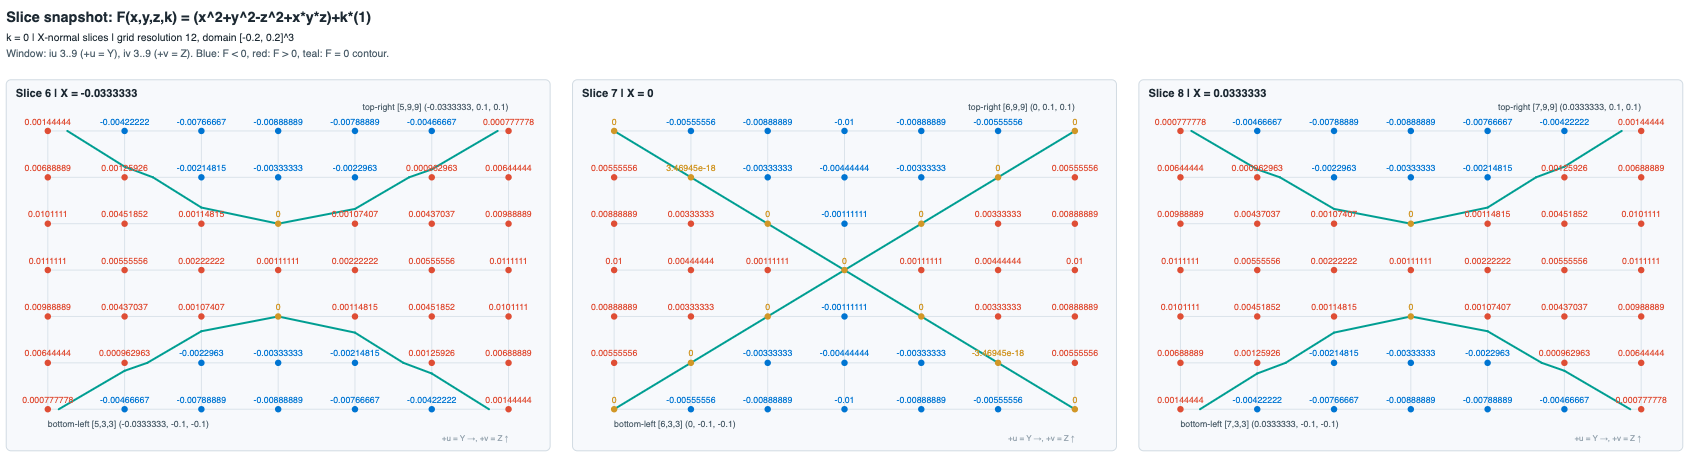
\includegraphics[width=\textwidth]{pictures/report/snap_A1_k0.png}\\[4pt]
    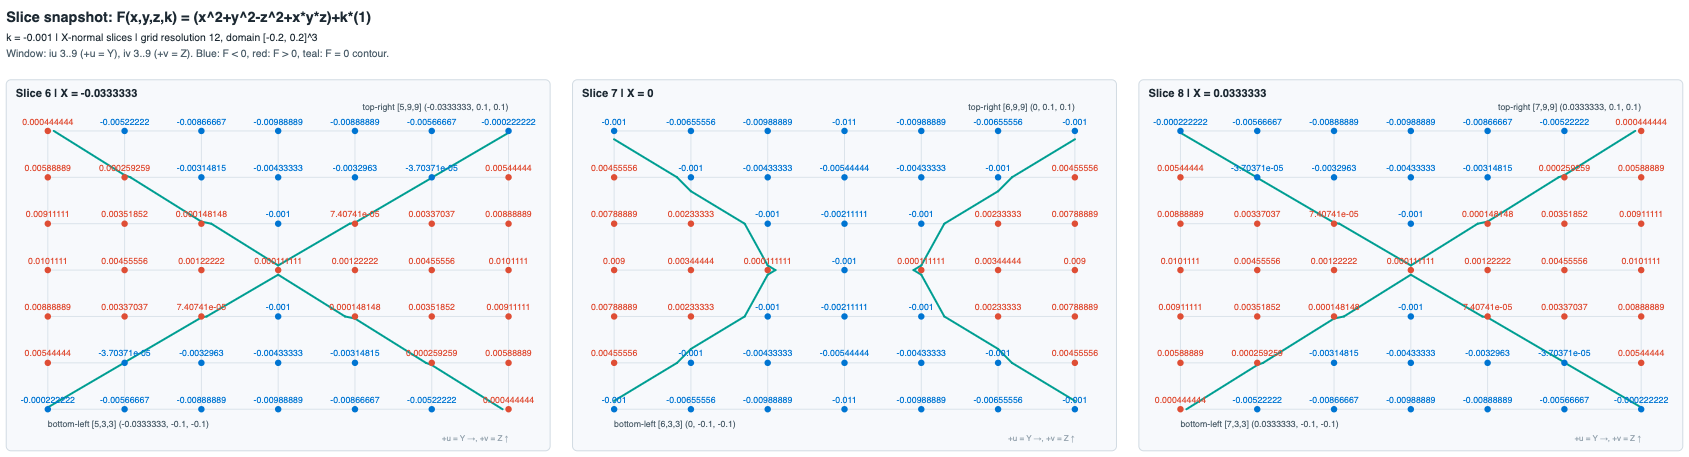
\includegraphics[width=\textwidth]{pictures/report/snap_A1_kneg.png}\\[4pt]
    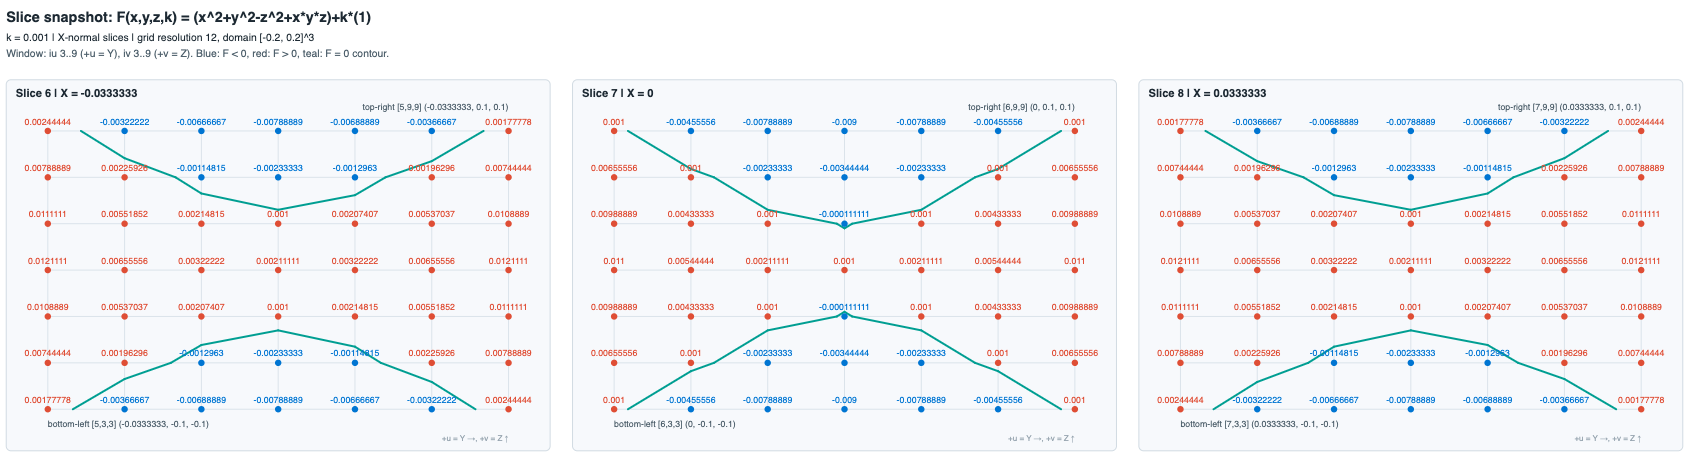
\includegraphics[width=\textwidth]{pictures/report/snap_A1_kpos.png}
    \caption{Slice snapshots around the singular point of $x^2+y^2-z^2+xyz+kG$ with $G=1$:
    $k=0$ (top), $k<0$ (middle), $k>0$ (bottom); the values of $k$, the grid and
    the window are printed in each snapshot. Every node shows its value (blue
    negative, red positive, yellow zero); teal is the zero level $S_k$.}
    \label{fig:r-A1-snap}
\end{figure}

\begin{table}[!h]
\centering
\footnotesize
\begin{adjustbox}{max width=\textwidth}
\begin{tabular}{l c l c c c c c c c}
\toprule
& & & & \multicolumn{2}{c}{$k<0$} & \multicolumn{2}{c}{$k>0$} & & \\
\cmidrule(lr){5-6}\cmidrule(lr){7-8}
$G$ & $m$ & essential part & predicted $\alpha$ & $\alpha$ & $C$ & $\alpha$ & $C$ & spread over $N$ & agrees \\
\midrule
$1$ & 0 & $1$ & $\tfrac12$ & 0.500{\scriptsize$\pm$0.000} & 1.00 & 0.500{\scriptsize$\pm$0.000} & 1.00 & 0.000 & yes \\
$x$ & 1 & $0$ & $1$ & 1.000{\scriptsize$\pm$0.000} & 0.71 & 1.000{\scriptsize$\pm$0.000} & 0.71 & 0.000 & yes \\
$y$ & 1 & $0$ & $1$ & 1.000{\scriptsize$\pm$0.000} & 0.71 & 1.000{\scriptsize$\pm$0.000} & 0.71 & 0.000 & yes \\
$z$ & 1 & $0$ & $1$ & 1.000{\scriptsize$\pm$0.000} & 0.71 & 1.000{\scriptsize$\pm$0.000} & 0.71 & 0.000 & yes \\
$x+y$ & 1 & $0$ & $1$ & 1.000{\scriptsize$\pm$0.001} & 1.00 & 1.000{\scriptsize$\pm$0.001} & 1.00 & 0.000 & yes \\
$x+z$ & 1 & $0$ & $1$ & 1.000{\scriptsize$\pm$0.000} & 0.71 & 1.000{\scriptsize$\pm$0.000} & 0.71 & 0.000 & yes \\
$x+y+z$ & 1 & $0$ & $1$ & 1.003{\scriptsize$\pm$0.004} & 1.01 & 1.003{\scriptsize$\pm$0.004} & 1.01 & 0.000 & yes \\
$2x-y+3z$ & 1 & $0$ & $1$ & 1.000{\scriptsize$\pm$0.001} & 2.12 & 1.000{\scriptsize$\pm$0.001} & 2.12 & 0.000 & yes \\
$x^2$ & 2 & $0$ & $1$ & 1.001{\scriptsize$\pm$0.000} & 0.06 & 0.999{\scriptsize$\pm$0.000} & 0.06 & 0.000 & yes \\
$x^2+y^2-z^2$ & 2 & $0$ & $1$ & 1.002{\scriptsize$\pm$0.001} & 0.01 & 0.998{\scriptsize$\pm$0.001} & 0.01 & 0.000 & yes \\
$xy$ & 2 & $0$ & $1$ & 1.000{\scriptsize$\pm$0.000} & 0.03 & 1.000{\scriptsize$\pm$0.000} & 0.03 & 0.000 & yes \\
$x^3$ & 3 & $0$ & $1$ & 1.000{\scriptsize$\pm$0.000} & 0.01 & 1.000{\scriptsize$\pm$0.000} & 0.01 & 0.000 & yes \\
$x^2y+y^2z+z^2x$ & 3 & $0$ & $1$ & 1.000{\scriptsize$\pm$0.000} & 0.02 & 1.000{\scriptsize$\pm$0.000} & 0.02 & 0.000 & yes \\
$F$ & -- & $0$ & $1$ & $S_k=S_0$ & -- & $S_k=S_0$ & -- & -- & yes \\
\bottomrule
\end{tabular}
\end{adjustbox}
\caption[Rates for $x^2+y^2-z^2+xyz$]{All perturbations of $F=x^2+y^2-z^2+xyz$: convergence rates (resolution $128$). Columns are explained in Section~\ref{sec:r-read}.}
\label{tab:r-A1-rates}
\end{table}
\begin{table}[!h]
\centering
\footnotesize
\begin{adjustbox}{max width=\textwidth}
\begin{tabular}{l l c l l c}
\toprule
$G$ & $P$ for $k\neq0$ & corank at $P$ & singular points, $k<0$ & singular points, $k>0$ & MC error \\
\midrule
$1$ & leaves $S_k$ & -- & none & none & 0.0010 \\
$x$ & regular & -- & none & none & 0.0025 \\
$y$ & regular & -- & none & none & 0.0025 \\
$z$ & regular & -- & none & none & 0.0024 \\
$x+y$ & regular & -- & none & none & 0.0036 \\
$x+z$ & regular & -- & none & none & 0.0022 \\
$x+y+z$ & regular & -- & none & none & 0.0035 \\
$2x-y+3z$ & regular & -- & none & none & 0.0020 \\
$x^2$ & singular & 0 ($A_1$) & only $P$ & only $P$ & 0.0014 \\
$x^2+y^2-z^2$ & singular & 0 ($A_1$) & only $P$ & only $P$ & 0.0014 \\
$xy$ & singular & 0 ($A_1$) & only $P$ & only $P$ & 0.0015 \\
$x^3$ & singular & 0 ($A_1$) & only $P$ & only $P$ & 0.0014 \\
$x^2y+y^2z+z^2x$ & singular & 0 ($A_1$) & only $P$ & only $P$ & 0.0013 \\
$F$ & singular & 0 ($A_1$) & only $P$ & only $P$ & 0.0014 \\
\bottomrule
\end{tabular}
\end{adjustbox}
\caption[Singular points for $x^2+y^2-z^2+xyz$]{All perturbations of $F=x^2+y^2-z^2+xyz$: the point $P$, the singular points of $S_k$ and the accuracy of Marching Cubes. Columns are explained in Section~\ref{sec:r-read}.}
\label{tab:r-A1-points}
\end{table}

The constant perturbation $G=1$ turns the double cone into a hyperboloid. For $k<0$ the equation reads, near the origin, $x^2+y^2-z^2=|k|$, one sheet with a narrow waist of radius $\sqrt{|k|}$; for $k>0$ it reads $x^2+y^2-z^2=-k$, two separate bowls with tips at $z=\pm\sqrt k$. Either way the change happens at the distance $\sqrt{|k|}$ from the old tip, so $\alpha=\tfrac12$. The measured value is $0.500$ with $C=1.00$ on both sides. The snapshots (Figure~\ref{fig:r-A1-snap}) show the hyperbola on the plane $x=0$: for $k<0$ the two branches open sideways, for $k>0$ up and down.

Every linear perturbation is inessential here, and all of them give $\alpha=1.000$ (to $\pm0.003$) on both sides. The origin stays on the surface but becomes regular. Completing the square shows why the rate is $1$: $x^2+kx=(x+\tfrac k2)^2-\tfrac{k^2}{4}$, so the cone is shifted by $k/2$ and opened by the constant $-k^2/4$, which acts at the distance $\sqrt{k^2/4}=|k|/2$ (Section~\ref{sec:essential}). Both effects are proportional to $|k|$. The rate is the same for all linear $G$, but the constant is not: $C=0.71$ for a single coordinate, $1.00$ for $x+y$ and $2.12$ for $2x-y+3z$, because the shift grows with the coefficients of $G$.

The perturbations of order two and three keep $P$ an ordinary double point (corank $0$ in Table~\ref{tab:r-A1-points}). The cone is only bent, by a distance proportional to $|k|$, so $\alpha=1$, with small constants between $0.01$ and $0.06$. This is the case $d_w(G)\ge1$ of the scaling estimate.

No perturbation creates a singular point other than $P$. This agrees with $\mu=1$ and Theorem~\ref{thm:conservation}: near $P$ there is only one stationary point to begin with, so nothing can split off. The Marching Cubes error stays between $0.0010$ and $0.0036$, below one grid cell, for every perturbation; the problems of Marching Cubes with this surface concern its topology, which is discussed in Section~\ref{sec:r-cone-results}.
\clearpage

% -----------------------------------------------------------------------------
\section{The Cusp $x^2+y^2+z^3$}
\label{sec:r-A2a}

Near the origin the surface is $x^2+y^2=-z^3$: for each $z<0$ the cross-section is a circle of radius $|z|^{3/2}$, and for $z>0$ there is nothing. The surface is therefore a thin horn that ends in a sharp tip at the origin (Figure~\ref{fig:r-A2a-exact}, slice $y=0$). The weights are $(\tfrac12,\tfrac12,\tfrac13)$: shrinking $z$ by $t^{1/3}$ and $x,y$ by $t^{1/2}$ keeps the equation. The Tjurina basis is $\{1,z\}$, so a constant and the $z$ direction are the only essential perturbations, while $x$ and $y$ are inessential. The predicted ranges are $[\tfrac13,\tfrac12]$ for $G=1$, $[\tfrac12,\tfrac34]$ for $G=z$ and $[\tfrac23,1]$ for $G=x$ and $G=y$.

\begin{figure}[!h]
\centering
\begin{minipage}[c]{0.18\textwidth}\centering
      \centering
    \resizebox{\linewidth}{!}{\panel{exact_A2a_k0.png}} \\[2pt]
    {\footnotesize $k=0$}
\end{minipage}\hfill
\begin{minipage}[c]{0.72\textwidth}\centering
\begin{adjustbox}{max width=\textwidth}
\begin{tabular}{c c c}
$G$ & $k=-0.01$ & $k=+0.01$ \\
$1$ & \panel{exact_A2a_1_neg.png} & \panel{exact_A2a_1_pos.png} \\
$z$ & \panel{exact_A2a_z_neg.png} & \panel{exact_A2a_z_pos.png} \\
$x$ & \panel{exact_A2a_x_neg.png} & \panel{exact_A2a_x_pos.png} \\
\end{tabular}
\end{adjustbox}
\end{minipage}
\caption{Exact slices of $S_k$ on the plane $y=0$ (horizontal axis $x$, vertical
axis $z$, both from $-0.25$ to $0.25$), computed from the polynomial. Grey: the
singular surface $S_0$; blue: $S_k$; red: singular points of $S_k$ found by the
numerical stationary-point search; cross: the origin.}
\label{fig:r-A2a-exact}
\end{figure}

\begin{figure}[!h]
    \centering
    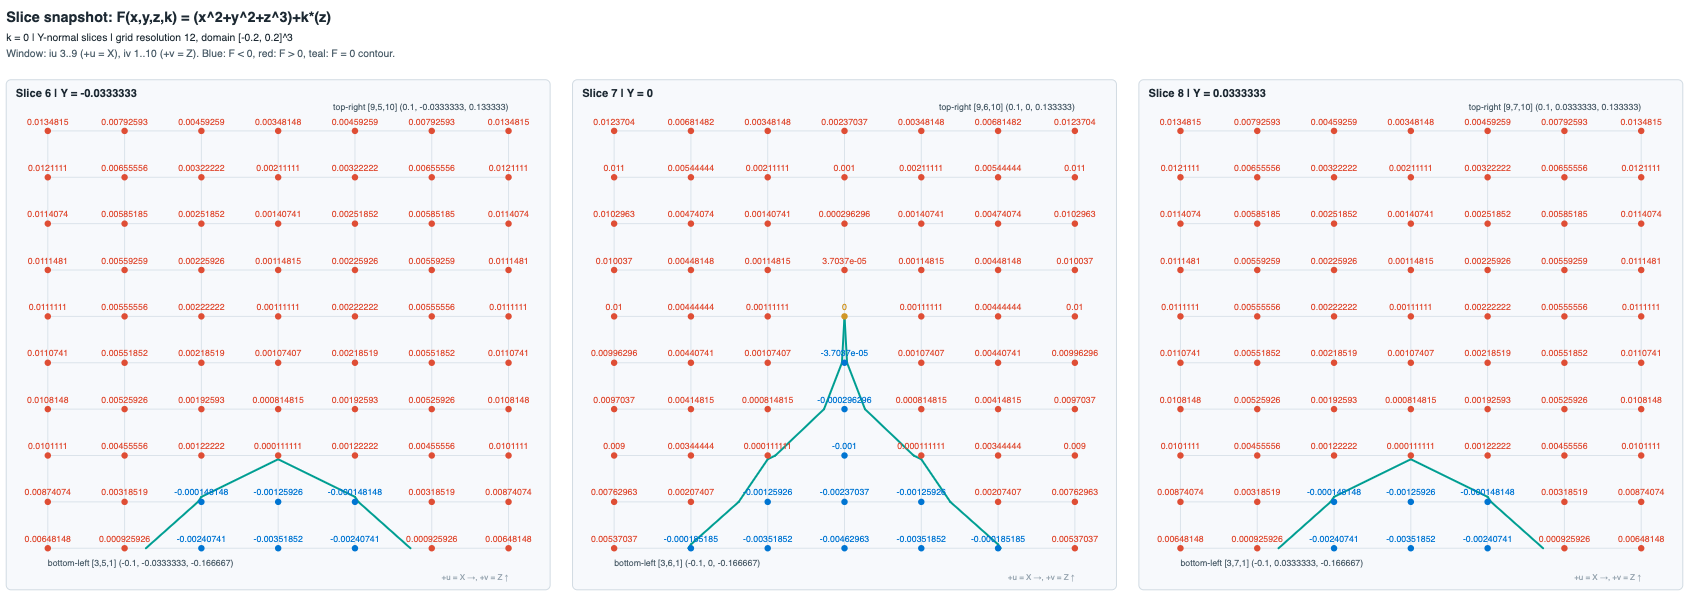
\includegraphics[width=\textwidth]{pictures/report/snap_A2a_k0.png}\\[4pt]
    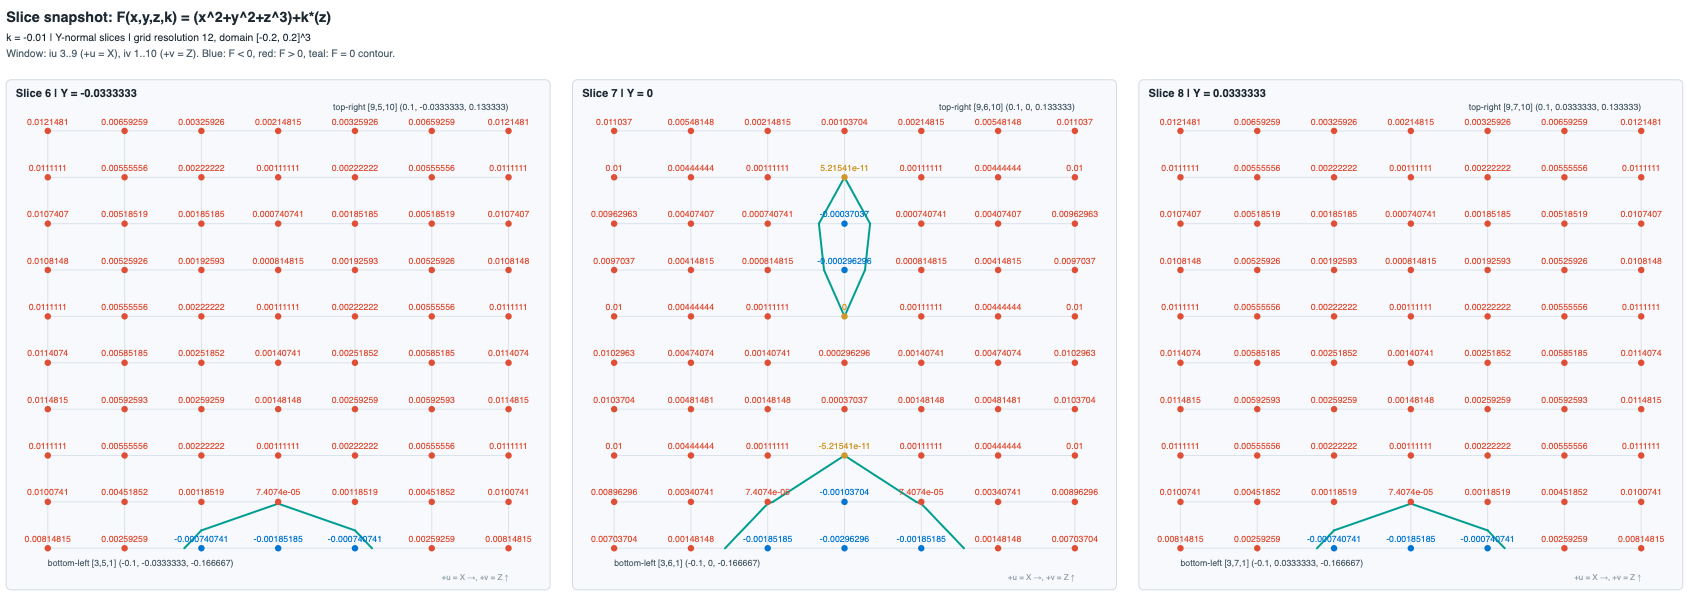
\includegraphics[width=\textwidth]{pictures/report/snap_A2a_kneg.png}\\[4pt]
    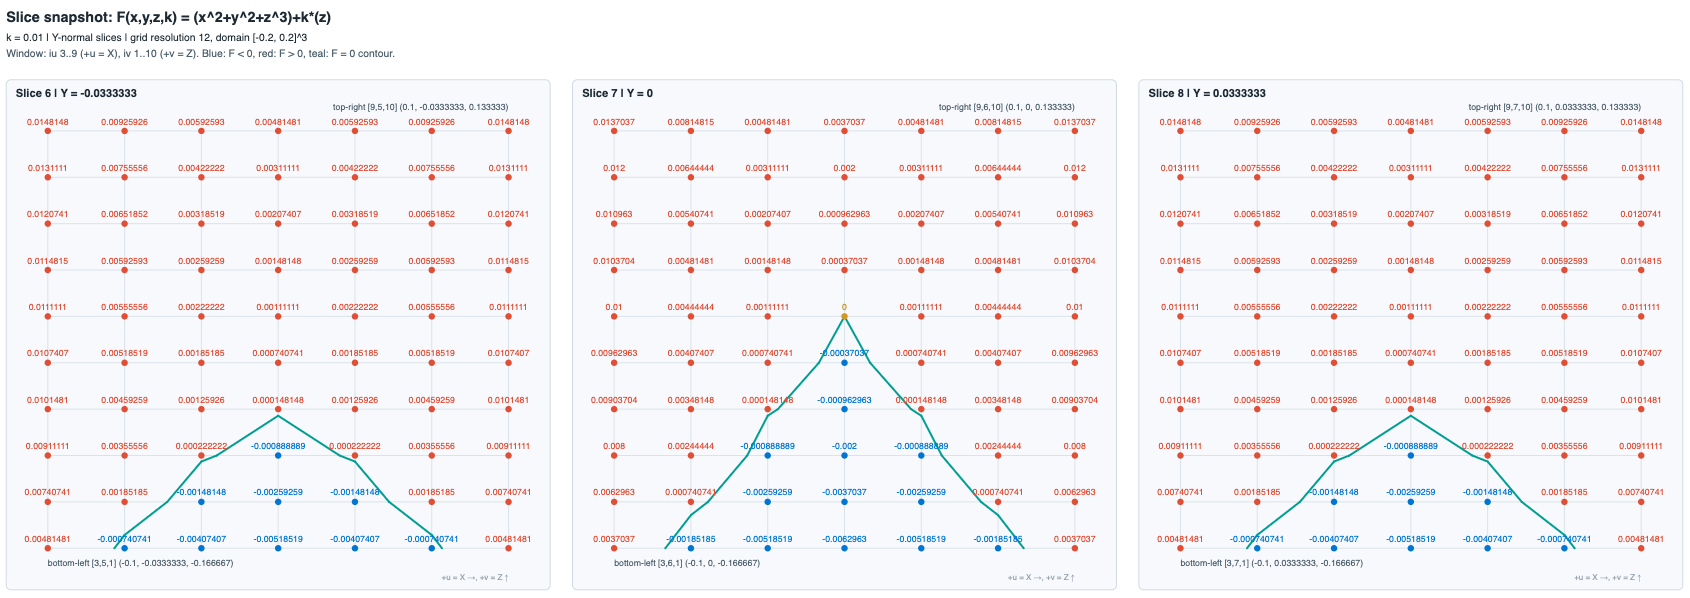
\includegraphics[width=\textwidth]{pictures/report/snap_A2a_kpos.png}
    \caption{Slice snapshots around the singular point of $x^2+y^2+z^3+kG$ with $G=z$:
    $k=0$ (top), $k<0$ (middle), $k>0$ (bottom); the values of $k$, the grid and
    the window are printed in each snapshot. Every node shows its value (blue
    negative, red positive, yellow zero); teal is the zero level $S_k$.}
    \label{fig:r-A2a-snap}
\end{figure}

\begin{table}[!h]
\centering
\footnotesize
\begin{adjustbox}{max width=\textwidth}
\begin{tabular}{l c l c c c c c c c}
\toprule
& & & & \multicolumn{2}{c}{$k<0$} & \multicolumn{2}{c}{$k>0$} & & \\
\cmidrule(lr){5-6}\cmidrule(lr){7-8}
$G$ & $m$ & essential part & predicted $\alpha$ & $\alpha$ & $C$ & $\alpha$ & $C$ & spread over $N$ & agrees \\
\midrule
$1$ & 0 & $1$ & $[\tfrac13,\tfrac12]$ & 0.341{\scriptsize$\pm$0.016} & 1.05 & 0.333{\scriptsize$\pm$0.000} & 1.00 & 0.044 & yes \\
$x$ & 1 & $0$ & $[\tfrac23,1]$ & 0.660{\scriptsize$\pm$0.026} & 0.59 & 0.660{\scriptsize$\pm$0.026} & 0.59 & 0.009 & yes \\
$y$ & 1 & $0$ & $[\tfrac23,1]$ & 0.660{\scriptsize$\pm$0.026} & 0.59 & 0.660{\scriptsize$\pm$0.026} & 0.59 & 0.009 & yes \\
$z$ & 1 & $z$ & $[\tfrac12,\tfrac34]$ & 0.500{\scriptsize$\pm$0.000} & 1.00 & 0.739{\scriptsize$\pm$0.003} & 0.40 & 0.000 & yes \\
$x+y$ & 1 & $0$ & $[\tfrac23,1]$ & 0.653{\scriptsize$\pm$0.051} & 0.70 & 0.653{\scriptsize$\pm$0.051} & 0.70 & 0.017 & yes \\
$x+z$ & 1 & $z$ & $[\tfrac12,\tfrac34]$ & 0.502{\scriptsize$\pm$0.001} & 1.02 & 0.787{\scriptsize$\pm$0.004} & 0.68 & 0.000 & \textbf{no} \\
$x+y+z$ & 1 & $z$ & $[\tfrac12,\tfrac34]$ & 0.505{\scriptsize$\pm$0.001} & 1.05 & 0.805{\scriptsize$\pm$0.006} & 0.83 & 0.000 & \textbf{no} \\
$2x-y+3z$ & 1 & $3z$ & $[\tfrac12,\tfrac34]$ & 0.502{\scriptsize$\pm$0.001} & 1.76 & 0.780{\scriptsize$\pm$0.002} & 1.44 & 0.000 & \textbf{no} \\
$x^2$ & 2 & $0$ & $1$ & 1.003{\scriptsize$\pm$0.002} & 0.03 & 0.999{\scriptsize$\pm$0.000} & 0.03 & 0.002 & yes \\
$x^2+y^2-z^2$ & 2 & $0$ & $1$ & 1.063{\scriptsize$\pm$0.044} & 0.71 & 1.000{\scriptsize$\pm$0.000} & 1.00 & 0.000 & yes \\
$xy$ & 2 & $0$ & $1$ & 1.001{\scriptsize$\pm$0.000} & 0.02 & 1.001{\scriptsize$\pm$0.000} & 0.02 & 0.000 & yes \\
$x^3$ & 3 & $0$ & $1$ & 1.000{\scriptsize$\pm$0.000} & 0.00 & 1.000{\scriptsize$\pm$0.000} & 0.00 & 0.000 & yes \\
$x^2y+y^2z+z^2x$ & 3 & $0$ & $1$ & 1.000{\scriptsize$\pm$0.000} & 0.01 & 1.000{\scriptsize$\pm$0.000} & 0.01 & 0.000 & yes \\
$F$ & -- & $0$ & $1$ & $S_k=S_0$ & -- & $S_k=S_0$ & -- & -- & yes \\
\bottomrule
\end{tabular}
\end{adjustbox}
\caption[Rates for $x^2+y^2+z^3$]{All perturbations of $F=x^2+y^2+z^3$: convergence rates (resolution $128$). Columns are explained in Section~\ref{sec:r-read}.}
\label{tab:r-A2a-rates}
\end{table}
\begin{table}[!h]
\centering
\footnotesize
\begin{adjustbox}{max width=\textwidth}
\begin{tabular}{l l c l l c}
\toprule
$G$ & $P$ for $k\neq0$ & corank at $P$ & singular points, $k<0$ & singular points, $k>0$ & MC error \\
\midrule
$1$ & leaves $S_k$ & -- & none & none & 0.0019 \\
$x$ & regular & -- & none & none & 0.0201 \\
$y$ & regular & -- & none & none & 0.0201 \\
$z$ & regular & -- & none & none & 0.0022 \\
$x+y$ & regular & -- & none & none & 0.0254 \\
$x+z$ & regular & -- & none & none & 0.0026 \\
$x+y+z$ & regular & -- & none & none & 0.0036 \\
$2x-y+3z$ & regular & -- & none & none & 0.0027 \\
$x^2$ & singular & 1 & only $P$ & only $P$ & 0.0021 \\
$x^2+y^2-z^2$ & singular & 0 ($A_1$) & only $P$ & only $P$ & 0.0080 \\
$xy$ & singular & 1 & only $P$ & only $P$ & 0.0021 \\
$x^3$ & singular & 1 & only $P$ & only $P$ & 0.0021 \\
$x^2y+y^2z+z^2x$ & singular & 1 & only $P$ & only $P$ & 0.0021 \\
$F$ & singular & 1 & only $P$ & only $P$ & 0.0021 \\
\bottomrule
\end{tabular}
\end{adjustbox}
\caption[Singular points for $x^2+y^2+z^3$]{All perturbations of $F=x^2+y^2+z^3$: the point $P$, the singular points of $S_k$ and the accuracy of Marching Cubes. Columns are explained in Section~\ref{sec:r-read}.}
\label{tab:r-A2a-points}
\end{table}

The constant perturbation moves the tip of the horn along the $z$-axis: $x^2+y^2=-z^3-k$ has its tip at $z=-k^{1/3}$. The distance is $|k|^{1/3}$, the lower end of the predicted range $[\tfrac13,\tfrac12]$, and the measurement gives $0.341$ for $k<0$ and $0.333$ for $k>0$, with $C\approx1$. The horn can only move along its axis, so the smallest weight decides.

The essential direction $z$ behaves differently on the two sides. For $k<0$ the cubic $z^3+kz$ gets two new real zeros $z=\pm\sqrt{|k|}$, and the horn \emph{splits open} along the axis over a length $\sqrt{|k|}$, so $\alpha=0.500$. For $k>0$ there are no new zeros, the horn only gets thicker, and the change is visible only across the axis, on the scale $|k|^{3/4}$; the measurement gives $0.739$, the upper end $\tfrac34$ (Figure~\ref{fig:r-A2a-snap}). The inessential directions $x$ and $y$ do not change the type of the singularity but create a \emph{spike}. Completing the square, $(x+\tfrac k2)^2+y^2=\tfrac{k^2}{4}-z^3$ is the horn shifted by $k/2$ plus a thin spike of radius about $|k|/2$ that reaches the height $(k^2/4)^{1/3}$ above the old tip ($0.029$ for $|k|=0.01$; Figure~\ref{fig:r-A2a-exact}, bottom row). Its height grows like $|k|^{2/3}$, and the measured rate is $0.660$, the lower end $\tfrac23$. The mixed perturbations $x+z$, $x+y+z$ and $2x-y+3z$ have the essential part $z$ (or $3z$) and behave like $z$ for $k<0$. For $k>0$ they give $0.78$--$0.81$, slightly above $\tfrac34$; these are the three ``no'' entries of Table~\ref{tab:r-A2a-rates}. Their inessential part shifts the surface by $O(|k|)$ at the same time as the essential part acts with the rate $\tfrac34$, both effects are visible for $10^{-4}\le|k|\le10^{-2}$, and the fitted slope lies between the two (Section~\ref{sec:r-deviations}).

All perturbations of order two and three keep the origin singular and give $\alpha=1$. The perturbation $x^2+y^2-z^2$ even makes the origin an ordinary double point (corank $0$), because its term $-kz^2$ is stronger near the origin than $z^3$.

No singular points other than $P$ appear, in agreement with $\mu=2$. The spike, however, is so thin that Marching Cubes misses it at every resolution. The extraction errors $0.0201$ for $G=x$ and $G=y$ and $0.0254$ for $G=x+y$ in Table~\ref{tab:r-A2a-points} are three to four grid cells, several times more than for the other perturbations, and they are exactly the part of the spike that is missing from the mesh.

The other two $A_2$ surfaces confirm this picture. For $x^3+y^3+z^2+x^2$, the same horn along the $y$-axis, every rate is the rate of $x^2+y^2+z^3$ with $y$ and $z$ exchanged, including the spike and its extraction error. This is the clearest confirmation that the rate depends only on the local type and on the essential part of $G$; the cubic term $x^3$ and the orientation of the horn make no difference. The saddle $x^2-y^2+z^3$ has the same complex type, but its quadratic part is indefinite, and the rates change. The constant opens the two crossing sheets sideways, so $G=1$ gives $0.500$ instead of $\tfrac13$, and the inessential $x$ and $y$ give $0.93$ instead of $0.66$, because the saddle has no tube for a spike to sit in. The perturbation $x+y$ even moves the cusp instead of opening it: $x^2-y^2+k(x+y)=(x+y)(x-y+k)$, so $S_k$ is the same pair of sheets with one of them shifted, and the singular point of type $A_2$ moves to $(-\tfrac k2,\tfrac k2,0)$ with $\gamma=1$.
\clearpage

% -----------------------------------------------------------------------------
\section{The $D_4$ Point with Three Lines: $x^2+y^3-3yz^2$}
\label{sec:r-D4b}

The $x$-direction is an ordinary quadratic direction, and the cubic part $y^3-3yz^2=y(y-\sqrt3z)(y+\sqrt3z)$ has three real linear factors. On the plane $x=0$ the surface is therefore three lines through the origin at $60^\circ$ to each other (Figure~\ref{fig:r-D4b-exact}). In space the equation reads $x^2=-y(y^2-3z^2)$. Over the three sectors of the $(y,z)$-plane where the cubic is negative the surface consists of two sheets $x=\pm\sqrt{-y(y^2-3z^2)}$ that meet along the bounding lines, so near $P$ the surface is made of three pieces pinched together at $P$, and its link has three components. The weights are $(\tfrac12,\tfrac13,\tfrac13)$, the Milnor number is $4$ and the Tjurina basis is $\{1,y,z,z^2\}$: the directions $y$ and $z$ are essential, $x$ is not. The predicted ranges are $[\tfrac13,\tfrac12]$ for $G=1$, $[\tfrac12,\tfrac34]$ for $G=y$ and $G=z$, and $[\tfrac23,1]$ for $G=x$.

\begin{figure}[!h]
\centering
\begin{minipage}[c]{0.18\textwidth}\centering
      \centering
    \resizebox{\linewidth}{!}{\panel{exact_D4b_k0.png}} \\[2pt]
    {\footnotesize $k=0$}
\end{minipage}\hfill
\begin{minipage}[c]{0.72\textwidth}\centering
\begin{adjustbox}{max width=\textwidth}
\begin{tabular}{c c c}
$G$ & $k=-0.01$ & $k=+0.01$ \\
$1$ & \panel{exact_D4b_1_neg.png} & \panel{exact_D4b_1_pos.png} \\
$y$ & \panel{exact_D4b_y_neg.png} & \panel{exact_D4b_y_pos.png} \\
$z$ & \panel{exact_D4b_z_neg.png} & \panel{exact_D4b_z_pos.png} \\
\end{tabular}
\end{adjustbox}
\end{minipage}
\caption{Exact slices of $S_k$ on the plane $x=0$ (horizontal axis $y$, vertical
axis $z$, both from $-0.25$ to $0.25$), computed from the polynomial. Grey: the
singular surface $S_0$; blue: $S_k$; red: singular points of $S_k$ found by the
numerical stationary-point search; cross: the origin.}
\label{fig:r-D4b-exact}
\end{figure}

\begin{figure}[!h]
    \centering
    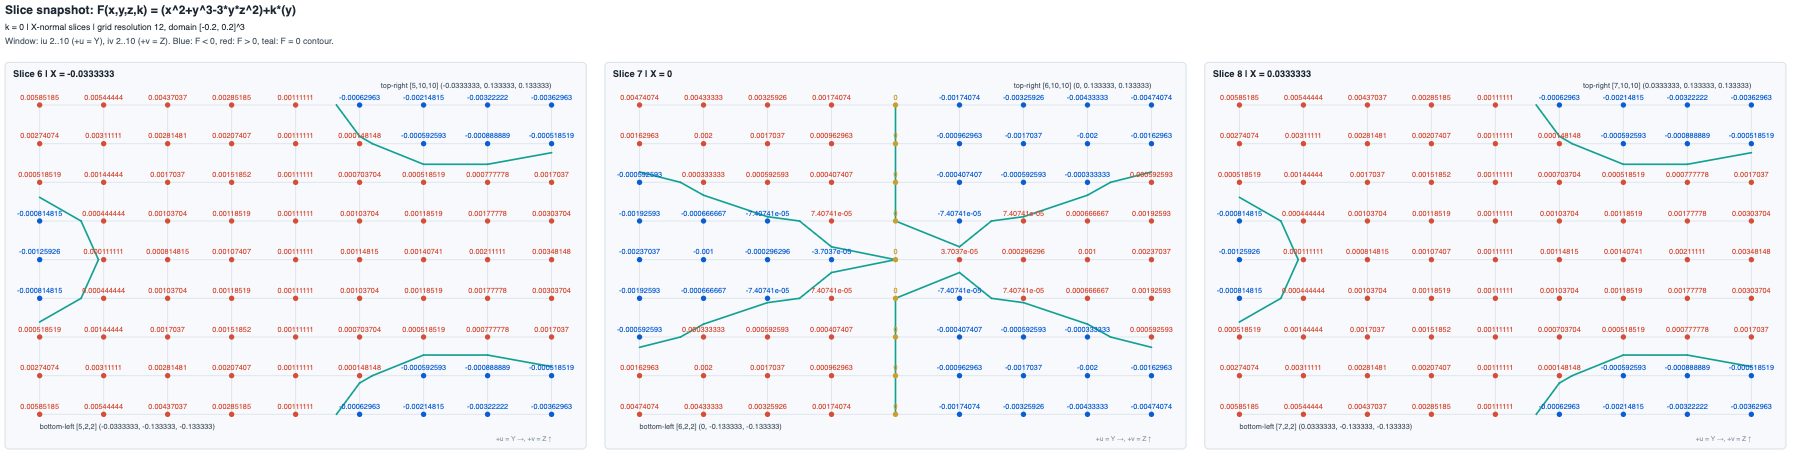
\includegraphics[width=\textwidth]{pictures/report/snap_D4b_k0.png}\\[4pt]
    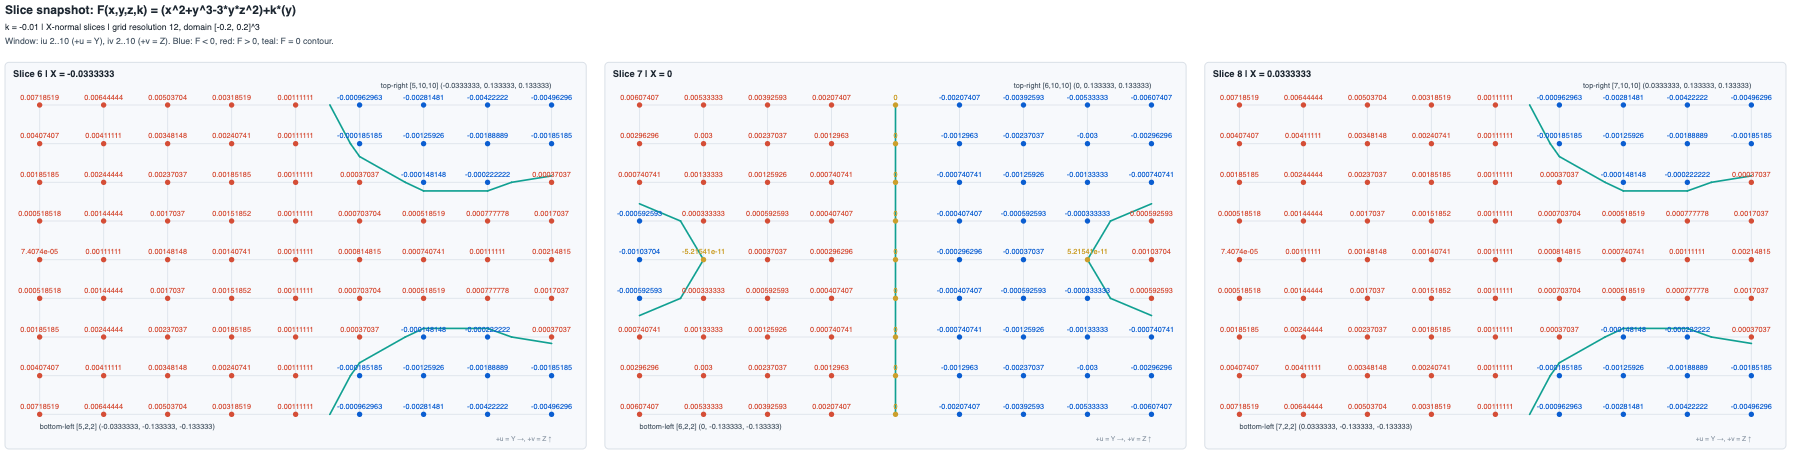
\includegraphics[width=\textwidth]{pictures/report/snap_D4b_kneg.png}\\[4pt]
    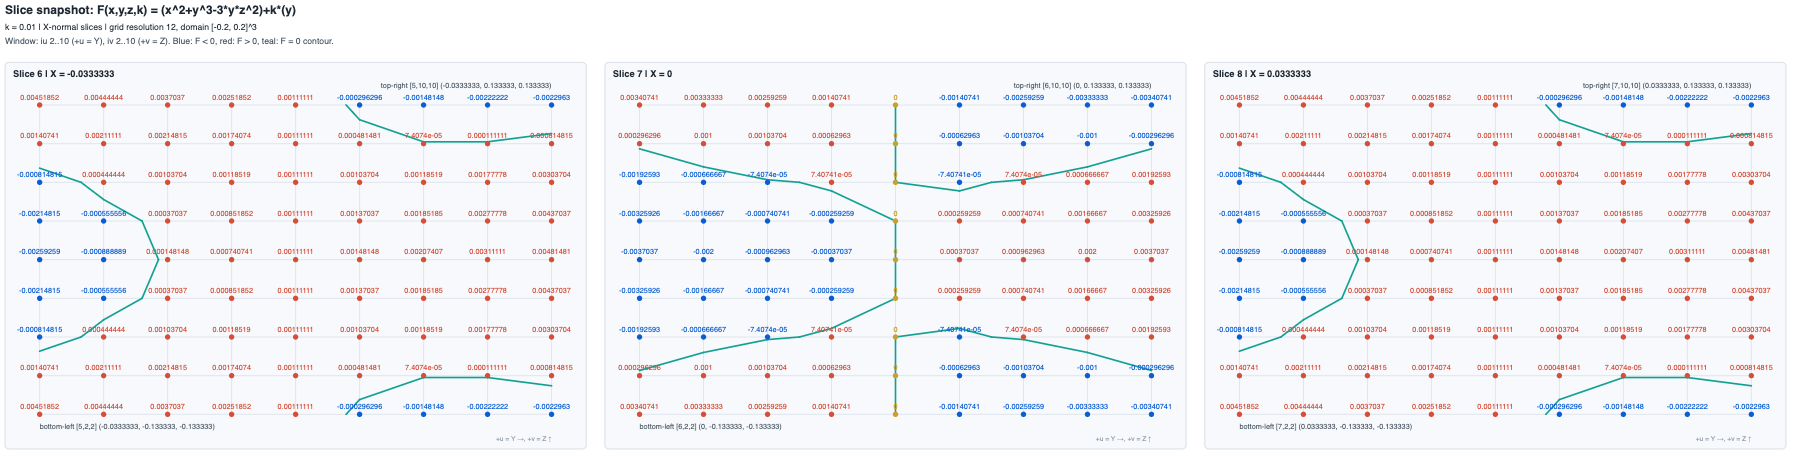
\includegraphics[width=\textwidth]{pictures/report/snap_D4b_kpos.png}
    \caption{Slice snapshots around the singular point of $x^2+y^3-3yz^2+kG$ with $G=y$:
    $k=0$ (top), $k<0$ (middle), $k>0$ (bottom); the values of $k$, the grid and
    the window are printed in each snapshot. Every node shows its value (blue
    negative, red positive, yellow zero); teal is the zero level $S_k$.}
    \label{fig:r-D4b-snap}
\end{figure}

\begin{table}[!h]
\centering
\footnotesize
\begin{adjustbox}{max width=\textwidth}
\begin{tabular}{l c l c c c c c c c}
\toprule
& & & & \multicolumn{2}{c}{$k<0$} & \multicolumn{2}{c}{$k>0$} & & \\
\cmidrule(lr){5-6}\cmidrule(lr){7-8}
$G$ & $m$ & essential part & predicted $\alpha$ & $\alpha$ & $C$ & $\alpha$ & $C$ & spread over $N$ & agrees \\
\midrule
$1$ & 0 & $1$ & $[\tfrac13,\tfrac12]$ & 0.332{\scriptsize$\pm$0.001} & 0.50 & 0.333{\scriptsize$\pm$0.001} & 1.00 & 0.001 & yes \\
$x$ & 1 & $0$ & $[\tfrac23,1]$ & 0.676{\scriptsize$\pm$0.011} & 0.34 & 0.676{\scriptsize$\pm$0.013} & 0.34 & 0.001 & yes \\
$y$ & 1 & $y$ & $[\tfrac12,\tfrac34]$ & 0.501{\scriptsize$\pm$0.004} & 0.53 & 0.504{\scriptsize$\pm$0.005} & 0.40 & 0.005 & yes \\
$z$ & 1 & $z$ & $[\tfrac12,\tfrac34]$ & 0.501{\scriptsize$\pm$0.005} & 0.53 & 0.501{\scriptsize$\pm$0.005} & 0.53 & 0.005 & yes \\
$x+y$ & 1 & $y$ & $[\tfrac12,\tfrac34]$ & 0.498{\scriptsize$\pm$0.004} & 0.51 & 0.493{\scriptsize$\pm$0.007} & 0.36 & 0.004 & yes \\
$x+z$ & 1 & $z$ & $[\tfrac12,\tfrac34]$ & 0.497{\scriptsize$\pm$0.005} & 0.51 & 0.497{\scriptsize$\pm$0.005} & 0.51 & 0.003 & yes \\
$x+y+z$ & 1 & $y + z$ & $[\tfrac12,\tfrac34]$ & 0.495{\scriptsize$\pm$0.002} & 0.54 & 0.499{\scriptsize$\pm$0.003} & 0.64 & 0.007 & yes \\
$2x-y+3z$ & 1 & $-y + 3z$ & $[\tfrac12,\tfrac34]$ & 0.499{\scriptsize$\pm$0.003} & 0.95 & 0.498{\scriptsize$\pm$0.005} & 0.80 & 0.004 & yes \\
$x^2$ & 2 & $0$ & $1$ & 1.002{\scriptsize$\pm$0.001} & 0.04 & 0.999{\scriptsize$\pm$0.001} & 0.04 & 0.001 & yes \\
$x^2+y^2-z^2$ & 2 & $0$ & $1$ & 0.877{\scriptsize$\pm$0.181} & 0.26 & 0.633{\scriptsize$\pm$0.232} & 0.05 & 0.430 & \textbf{no} \\
$xy$ & 2 & $0$ & $1$ & 0.267{\scriptsize$\pm$0.312} & 0.00 & 0.267{\scriptsize$\pm$0.312} & 0.00 & 0.191 & \textbf{no} \\
$x^3$ & 3 & $0$ & $1$ & 1.000{\scriptsize$\pm$0.000} & 0.00 & 1.000{\scriptsize$\pm$0.000} & 0.00 & 0.000 & yes \\
$x^2y+y^2z+z^2x$ & 3 & $0$ & $1$ & 0.936{\scriptsize$\pm$0.359} & 0.05 & 0.809{\scriptsize$\pm$0.327} & 0.02 & 0.127 & yes \\
$F$ & -- & $0$ & $1$ & $S_k=S_0$ & -- & $S_k=S_0$ & -- & -- & yes \\
\bottomrule
\end{tabular}
\end{adjustbox}
\caption[Rates for $x^2+y^3-3yz^2$]{All perturbations of $F=x^2+y^3-3yz^2$: convergence rates (resolution $128$). Columns are explained in Section~\ref{sec:r-read}.}
\label{tab:r-D4b-rates}
\end{table}
\begin{table}[!h]
\centering
\footnotesize
\begin{adjustbox}{max width=\textwidth}
\begin{tabular}{l l c l l c}
\toprule
$G$ & $P$ for $k\neq0$ & corank at $P$ & singular points, $k<0$ & singular points, $k>0$ & MC error \\
\midrule
$1$ & leaves $S_k$ & -- & none & none & 0.0013 \\
$x$ & regular & -- & none & none & 0.0101 \\
$y$ & regular & -- & none & 2$\times$$A_1$, $\gamma=0.50$ & 0.0028 \\
$z$ & regular & -- & none & none & 0.0017 \\
$x+y$ & regular & -- & none & none & 0.0063 \\
$x+z$ & regular & -- & none & none & 0.0022 \\
$x+y+z$ & regular & -- & none & none & 0.0021 \\
$2x-y+3z$ & regular & -- & none & none & 0.0021 \\
$x^2$ & singular & 2 & only $P$ & only $P$ & 0.0027 \\
$x^2+y^2-z^2$ & singular & 0 ($A_1$) & only $P$ & only $P$ & 0.0031 \\
$xy$ & singular & 1 & $P$; 1 more for some $k$ & $P$; 1 more for some $k$ & 0.0027 \\
$x^3$ & singular & 2 & only $P$ & only $P$ & 0.0027 \\
$x^2y+y^2z+z^2x$ & singular & 2 & only $P$ & only $P$ & 0.0027 \\
$F$ & singular & 2 & only $P$ & only $P$ & 0.0027 \\
\bottomrule
\end{tabular}
\end{adjustbox}
\caption[Singular points for $x^2+y^3-3yz^2$]{All perturbations of $F=x^2+y^3-3yz^2$: the point $P$, the singular points of $S_k$ and the accuracy of Marching Cubes. Columns are explained in Section~\ref{sec:r-read}.}
\label{tab:r-D4b-points}
\end{table}

The constant perturbation gives $0.332$ and $0.333$, the lower end $\tfrac13$, with $C=0.50$ for $k<0$ and $1.00$ for $k>0$. In the $y,z$-directions, where both weights are $\tfrac13$, the constant acts as on a cubic cone. The topology changes with the sign: for $k<0$ the equation $x^2=|k|-y(y^2-3z^2)$ has solutions over a neighbourhood of the origin, and the three pieces merge into one sheet, while for $k>0$ they move apart and stay three.

All essential linear perturbations give $\alpha\approx0.50$ on \emph{both} sides, with similar constants. Unlike the one-line case below, three real lines leave no direction in which the perturbation can only bend the surface: some pair of lines is always pulled apart on the scale $\sqrt{|k|}$. The inessential $G=x$ gives $0.676$. Completing the square, $(x+\tfrac k2)^2+y^3-3yz^2=\tfrac{k^2}{4}$, so the surface is shifted by $k/2$ and receives the constant $k^2/4$. On this surface a constant $c$ moves the surface by about $|c|^{1/3}$ (the rate $\tfrac13$ of $G=1$), so the constant $k^2/4$ moves it by about $(k^2/4)^{1/3}$, which is proportional to $|k|^{2/3}$, and the measured rate is close to this $\tfrac23$.

Of the perturbations of order two and three, $x^2$ and $x^3$ give $1.00$. For $xy$, $x^2+y^2-z^2$ and $x^2y+y^2z+z^2x$ the deformation is so small that the measured distance reaches the resolution of the measurement, and the fitted values $0.27$--$0.94$, two of them ``no'', describe the measurement rather than the surface (Section~\ref{sec:r-deviations}).

The perturbation $G=y$ creates two ordinary double points for $k>0$. The slice $x=0$ becomes $y(y^2-3z^2+k)=0$: the line $y=0$ and the hyperbola $y^2-3z^2=-k$, which meet at $(0,0,\pm\sqrt{k/3})$. At these points $\partial_yH_k=3y^2-3z^2+k=0$ and $\partial_zH_k=-6yz=0$, so they are singular points of $S_k$. They are found by the stationary-point search for every $k>0$ and move with $\gamma=0.50$ (Figures~\ref{fig:r-D4b-exact} and~\ref{fig:r-D4b-snap}). For $k<0$ the hyperbola opens the other way and does not meet the line. The point $P$ itself becomes regular, and the two double points carry two of the four units of the Milnor number.

The other $D_4$ surface, $x^2+y^3+z^3$, has a cubic part with only one real line, $y^3+z^3=(y+z)(y^2-yz+z^2)$, and the surface folds over this line and pinches at the origin. Its rates are the same, $\tfrac13$ and $\tfrac12$, but for the essential linear perturbations the constant is about four times larger for $k<0$ ($1.03$) than for $k>0$ ($0.28$): for $k<0$ the cubic $y^3+ky$ gets two new real zeros $\pm\sqrt{|k|}$ and the surface gets new sheets, for $k>0$ it only bends. The inessential $G=x$ gives $0.763$, between the $\tfrac23$ of the constant $k^2/4$ and the rate $1$ of the shift, and as for the horn this second-order effect is a thin part of the surface that Marching Cubes misses (extraction error $0.0226$). The perturbation $x^2+y^2-z^2$ creates one more ordinary double point. One checks that the stationary points of $x^2+y^3+z^3+k(x^2+y^2-z^2)$ are $(0,y,z)$ with $y\in\{0,-\tfrac{2k}3\}$ and $z\in\{0,\tfrac{2k}3\}$, all four real and non-degenerate. The value of $H_k$ vanishes at $P$ and at $(0,-\tfrac{2k}3,\tfrac{2k}3)$, which is the new singular point and moves with $\gamma=1$; at the other two stationary points $H_k=\pm\tfrac{4k^3}{27}\neq0$. So the four units of the Milnor number are split into $1+1+1+1$, and two of them are real stationary points that do not lie on the surface.
\clearpage

% -----------------------------------------------------------------------------
\section{The Fermat Cone $x^3+y^3+z^3$}
\label{sec:r-E6a}

The polynomial is a homogeneous cubic, so every line through the origin and a point of the surface lies on the surface: the surface is a \emph{cone} over the real cubic curve $x^3+y^3+z^3=0$ \cite{dimca1992singularities}. This does not mean that it looks like a circular cone; the shape depends on the curve. In the chart $z=1$ of the projective plane the Fermat curve is the graph $y=-\sqrt[3]{1+x^3}$ of a continuous function, closed up by one point at infinity, so it is a single closed curve that, like a projective line, cannot be contracted to a point. The cone over it is one wavy sheet through the origin (Figure~\ref{fig:r-E6a-iso}), smooth everywhere except at the origin, where all its lines meet. All weights are $\tfrac13$, $\mu=\tau=8$, and the essential directions are $1,x,y,z,xy,xz,yz,xyz$, while $x^2,y^2,z^2$ and the pure cubes are inessential. Because $F$ is homogeneous, a homogeneous $G$ of degree $m$ gives an exactly self-similar family for each sign of $k$ (Proposition~\ref{prop:self-similar}): $S_k$ is a fixed surface scaled by $|k|^{1/(3-m)}$, and the rates are exactly $\tfrac13$, $\tfrac12$ and $1$ for $m=0$, $1$ and $2$.

\begin{figure}[!h]
    \centering
    \begin{subfigure}{0.3\textwidth}\centering
        \thesisimage{pictures/ch3/cone_Fplus.png}{0.8\textwidth}{4cm}{$F_+$, $k=0$}
        \caption{$k=0$}\end{subfigure}
    \caption{$x^3+y^3+z^3$ extracted by Marching Cubes, coloured by $\|\nabla F\|$
    (blue: small gradient). The singular point is the dark spot in the middle.}
    \label{fig:r-E6a-iso}
\end{figure}

\begin{figure}[!h]
    \centering
    \begin{subfigure}{0.31\textwidth}\centering
        \thesisimage{pictures/ch4/G1_kneg.png}{0.85\textwidth}{4cm}{$F_++k$, $k<0$}
        \caption{$k<0$}\end{subfigure}\hfill
    \begin{subfigure}{0.31\textwidth}\centering
        \thesisimage{pictures/ch4/G1_k0.png}{0.85\textwidth}{4cm}{$F_+$, $k=0$}
        \caption{$k=0$}\end{subfigure}\hfill
    \begin{subfigure}{0.31\textwidth}\centering
        \thesisimage{pictures/ch4/G1_kpos.png}{0.85\textwidth}{4cm}{$F_++k$, $k>0$}
        \caption{$k>0$}\end{subfigure}
    \caption{$x^3+y^3+z^3+k$: the apex of the cone is replaced by a smooth cap
    (isosurfaces from the viewer, $|k|=0.005$).}
    \label{fig:r-E6a-G1}
\end{figure}

\begin{figure}[!h]
\centering
\begin{minipage}[c]{0.18\textwidth}\centering
      \centering
    \resizebox{\linewidth}{!}{\panel{exact_E6a_k0.png}} \\[2pt]
    {\footnotesize $k=0$}
\end{minipage}\hfill
\begin{minipage}[c]{0.72\textwidth}\centering
\begin{adjustbox}{max width=\textwidth}
\begin{tabular}{c c c}
$G$ & $k=-0.01$ & $k=+0.01$ \\
$1$ & \panel{exact_E6a_1_neg.png} & \panel{exact_E6a_1_pos.png} \\
$x+y$ & \panel{exact_E6a_xpy_neg.png} & \panel{exact_E6a_xpy_pos.png} \\
$x^2+y^2-z^2$ & \panel{exact_E6a_x2py2mz2_neg.png} & \panel{exact_E6a_x2py2mz2_pos.png} \\
\end{tabular}
\end{adjustbox}
\end{minipage}
\caption{Exact slices of $S_k$ on the plane $z=0$ (horizontal axis $x$, vertical
axis $y$, both from $-0.25$ to $0.25$), computed from the polynomial. Grey: the
singular surface $S_0$; blue: $S_k$; red: singular points of $S_k$ found by the
numerical stationary-point search; cross: the origin.}
\label{fig:r-E6a-exact}
\end{figure}

\begin{figure}[!h]
    \centering
    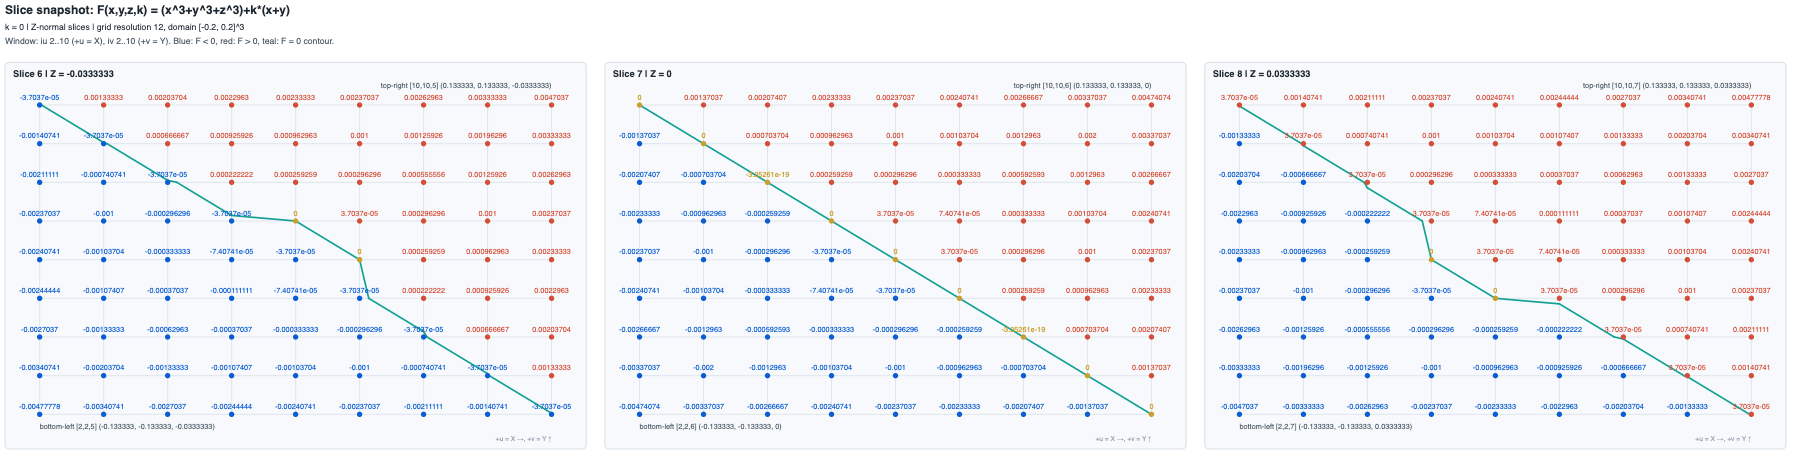
\includegraphics[width=\textwidth]{pictures/report/snap_E6a_k0.png}\\[4pt]
    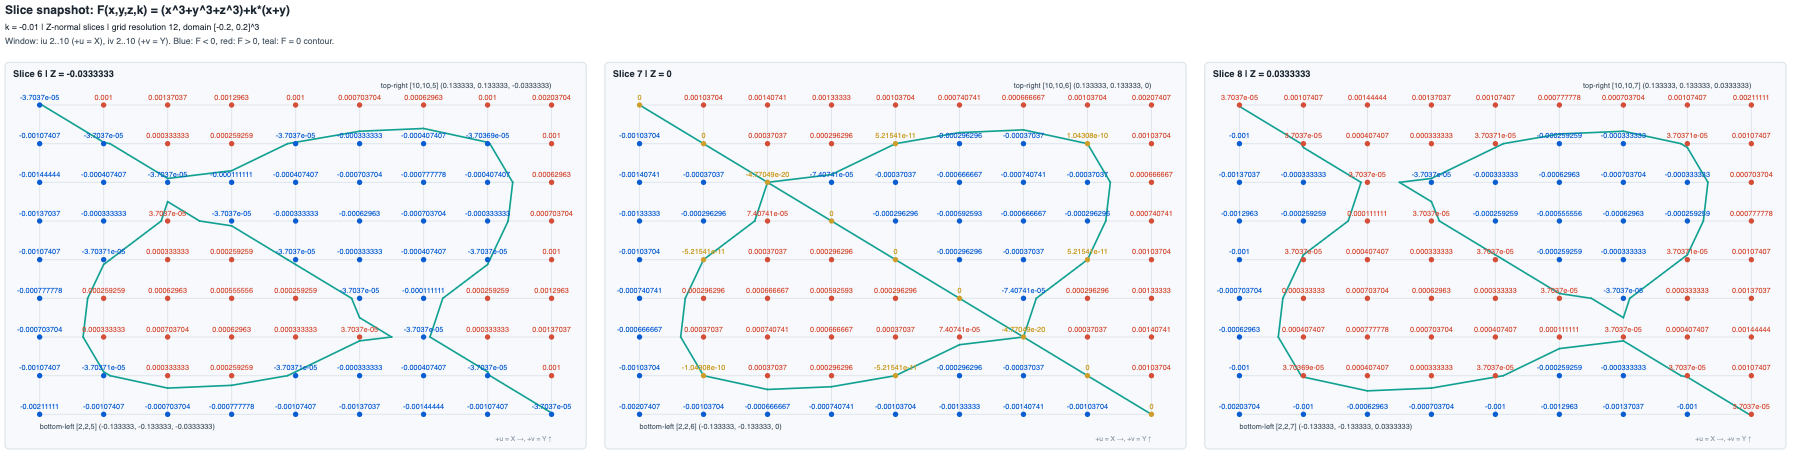
\includegraphics[width=\textwidth]{pictures/report/snap_E6a_kneg.png}\\[4pt]
    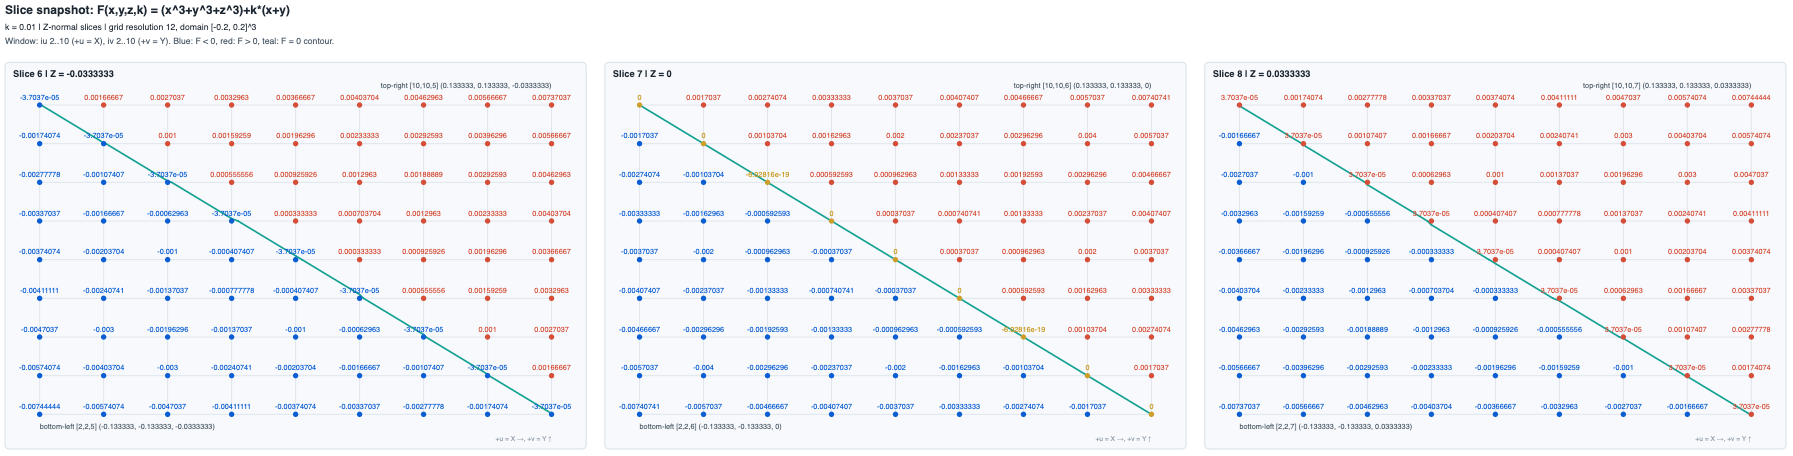
\includegraphics[width=\textwidth]{pictures/report/snap_E6a_kpos.png}
    \caption{Slice snapshots around the singular point of $x^3+y^3+z^3+kG$ with $G=x+y$:
    $k=0$ (top), $k<0$ (middle), $k>0$ (bottom); the values of $k$, the grid and
    the window are printed in each snapshot. Every node shows its value (blue
    negative, red positive, yellow zero); teal is the zero level $S_k$.}
    \label{fig:r-E6a-snap}
\end{figure}

\begin{table}[!h]
\centering
\footnotesize
\begin{adjustbox}{max width=\textwidth}
\begin{tabular}{l c l c c c c c c c}
\toprule
& & & & \multicolumn{2}{c}{$k<0$} & \multicolumn{2}{c}{$k>0$} & & \\
\cmidrule(lr){5-6}\cmidrule(lr){7-8}
$G$ & $m$ & essential part & predicted $\alpha$ & $\alpha$ & $C$ & $\alpha$ & $C$ & spread over $N$ & agrees \\
\midrule
$1$ & 0 & $1$ & $\tfrac13$ & 0.333{\scriptsize$\pm$0.007} & 1.16 & 0.333{\scriptsize$\pm$0.007} & 1.16 & 0.002 & yes \\
$x$ & 1 & $x$ & $\tfrac12$ & 0.501{\scriptsize$\pm$0.001} & 1.03 & 0.500{\scriptsize$\pm$0.000} & 0.29 & 0.001 & yes \\
$y$ & 1 & $y$ & $\tfrac12$ & 0.501{\scriptsize$\pm$0.001} & 1.03 & 0.500{\scriptsize$\pm$0.000} & 0.29 & 0.001 & yes \\
$z$ & 1 & $z$ & $\tfrac12$ & 0.501{\scriptsize$\pm$0.001} & 1.03 & 0.500{\scriptsize$\pm$0.000} & 0.29 & 0.001 & yes \\
$x+y$ & 1 & $x + y$ & $\tfrac12$ & 0.500{\scriptsize$\pm$0.000} & 1.38 & 0.500{\scriptsize$\pm$0.000} & 0.37 & 0.000 & yes \\
$x+z$ & 1 & $x + z$ & $\tfrac12$ & 0.500{\scriptsize$\pm$0.000} & 1.38 & 0.500{\scriptsize$\pm$0.000} & 0.37 & 0.000 & yes \\
$x+y+z$ & 1 & $x + y + z$ & $\tfrac12$ & 0.500{\scriptsize$\pm$0.000} & 1.69 & 0.500{\scriptsize$\pm$0.000} & 0.11 & 0.006 & yes \\
$2x-y+3z$ & 1 & $2x - y + 3z$ & $\tfrac12$ & 0.500{\scriptsize$\pm$0.000} & 2.00 & 0.500{\scriptsize$\pm$0.000} & 0.80 & 0.002 & yes \\
$x^2$ & 2 & $0$ & $1$ & 1.034{\scriptsize$\pm$0.035} & 1.11 & 1.006{\scriptsize$\pm$0.006} & 0.94 & 0.005 & yes \\
$x^2+y^2-z^2$ & 2 & $0$ & $1$ & 1.002{\scriptsize$\pm$0.003} & 1.12 & 1.002{\scriptsize$\pm$0.003} & 1.12 & 0.002 & yes \\
$xy$ & 2 & $xy$ & $1$ & 1.030{\scriptsize$\pm$0.032} & 0.74 & 0.996{\scriptsize$\pm$0.007} & 0.61 & 0.001 & yes \\
$x^3$ & 3 & $0$ & $1$ & 1.001{\scriptsize$\pm$0.000} & 0.05 & 0.999{\scriptsize$\pm$0.000} & 0.04 & 0.000 & yes \\
$x^2y+y^2z+z^2x$ & 3 & $0$ & $1$ & 1.000{\scriptsize$\pm$0.000} & 0.05 & 1.000{\scriptsize$\pm$0.000} & 0.05 & 0.000 & yes \\
$x+y+1.5874z$ & 1 & $x + y + 1.587z$ & $\tfrac12$ & 0.500{\scriptsize$\pm$0.000} & 1.84 & 0.500{\scriptsize$\pm$0.000} & 0.19 & 0.001 & yes \\
$F$ & -- & $0$ & $1$ & $S_k=S_0$ & -- & $S_k=S_0$ & -- & -- & yes \\
\bottomrule
\end{tabular}
\end{adjustbox}
\caption[Rates for $x^3+y^3+z^3$]{All perturbations of $F=x^3+y^3+z^3$: convergence rates (resolution $128$). Columns are explained in Section~\ref{sec:r-read}.}
\label{tab:r-E6a-rates}
\end{table}
\begin{table}[!h]
\centering
\footnotesize
\begin{adjustbox}{max width=\textwidth}
\begin{tabular}{l l c l l c}
\toprule
$G$ & $P$ for $k\neq0$ & corank at $P$ & singular points, $k<0$ & singular points, $k>0$ & MC error \\
\midrule
$1$ & leaves $S_k$ & -- & none & none & 0.0005 \\
$x$ & regular & -- & none & none & 0.0029 \\
$y$ & regular & -- & none & none & 0.0029 \\
$z$ & regular & -- & none & none & 0.0029 \\
$x+y$ & regular & -- & 2$\times$$A_2$, $\gamma=0.50$ & none & 0.0026 \\
$x+z$ & regular & -- & 2$\times$$A_2$, $\gamma=0.50$ & none & 0.0026 \\
$x+y+z$ & regular & -- & none & none & 0.0027 \\
$2x-y+3z$ & regular & -- & none & none & 0.0017 \\
$x^2$ & singular & 2 & only $P$ & only $P$ & 0.0036 \\
$x^2+y^2-z^2$ & singular & 0 ($A_1$) & $P$ + 2$\times$$A_1$, $\gamma=1.00$ & $P$ + 2$\times$$A_1$, $\gamma=1.00$ & 0.0059 \\
$xy$ & singular & 1 & only $P$ & only $P$ & 0.0064 \\
$x^3$ & singular & 3 & only $P$ & only $P$ & 0.0018 \\
$x^2y+y^2z+z^2x$ & singular & 3 & only $P$ & only $P$ & 0.0017 \\
$x+y+1.5874z$ & regular & -- & 2$\times$$A_1$, $\gamma=0.50$ & none & 0.0026 \\
$F$ & singular & 3 & only $P$ & only $P$ & 0.0019 \\
\bottomrule
\end{tabular}
\end{adjustbox}
\caption[Singular points for $x^3+y^3+z^3$]{All perturbations of $F=x^3+y^3+z^3$: the point $P$, the singular points of $S_k$ and the accuracy of Marching Cubes. Columns are explained in Section~\ref{sec:r-read}.}
\label{tab:r-E6a-points}
\end{table}

The constant perturbation replaces the apex by a smooth cap (Figure~\ref{fig:r-E6a-G1}). The distance from the origin to $S_k$ is exactly $|k|^{1/3}$, since the largest value of $x^3+y^3+z^3$ on the unit sphere is $1$. The Hausdorff distance is $1.163\,|k|^{1/3}$, because the cap is farthest from the cone in the direction $(1,1,1)$, and the measured rate is $0.333$, as predicted.

Every linear perturbation is essential and gives $0.500$ on both sides and at every resolution; the spread over $N$ is at most $0.006$. This is the self-similarity at work: only the constant depends on the direction of $G$. It is larger for $k<0$ ($1.03$ for $G=x$) than for $k>0$ ($0.29$), because for $k<0$ the cone opens with new real structure, while for $k>0$ it is only smoothed.

Every perturbation of order two or three gives $1.00$. The perturbation $x^2$ is inessential, a translation by $k/3$ (Section~\ref{sec:essential}), and the origin stays singular with corank $2$; $x^2+y^2-z^2$ makes the origin an ordinary double point, and $xy$ is essential and keeps it singular with corank $1$. The cubes stretch the cone, $x^3+kx^3=(\sqrt[3]{1+k}\,x)^3$, and $x^2y+y^2z+z^2x$ changes its shape; both keep the type of the singular point and have tiny constants ($0.05$).

The singular points agree exactly with Proposition~\ref{prop:linear}. The perturbations $x$, $y$, $z$, $x+y+z$ and $2x-y+3z$ create none. For $x+y$ and $x+z$ the balance condition is $1-1=0$, and two cusps ($A_2$) appear at $(\pm s,\mp s,0)$ with $s=\sqrt{|k|/3}$, for $k<0$ only, moving with $\gamma=0.500$. In the slice $z=0$ the surface is then the line $x=-y$ and an ellipse, and the cusps are where they meet (Figures~\ref{fig:r-E6a-exact} and~\ref{fig:r-E6a-snap}). The balanced perturbation $x+y+1.5874z$, with $1+1-(1.5874)^{3/2}=0$, creates two ordinary double points with $\gamma=0.500$. Of the perturbations of order two, $x^2+y^2-z^2$ adds two ordinary double points that move linearly ($\gamma=1$): all eight stationary points are then real, and together with $P$ three of the eight units of the Milnor number become real singular points.

The other three cones behave in the same way. The mirrored cone $x^3+y^3-z^3$ gives, by the reflection \eqref{eq:reflection}, the numbers of $x^3+y^3+z^3$ with $z$ replaced by $-z$ in $G$; so $x+z$ becomes a different perturbation and creates no singular points, and the balanced direction is $x+y-1.5874z$. The non-diagonal cones $x^3+y^3+z^3+xyz$ and $x^3+2y^3+3z^3+2xyz$ give exactly the same rates, $\tfrac13$, $\tfrac12$ and $1$, on both sides, and differ only in the constants and in which linear perturbations create singular points. For them $x+y$ does \emph{not} create cusps, because the mixed term $xyz$ moves the directions in which a stationary point lies on the surface, and the direction search found their own balanced perturbations $x+y+2z$ and $x+y+2.6581z$, each creating two ordinary double points with $\gamma=0.500$. Without the search there would be no way to guess these coefficients.
\clearpage

% -----------------------------------------------------------------------------
\section{All Surfaces and Perturbations Compared}
\label{sec:r-groupF}

Looking at all ten surfaces together, they fall into five groups (Table~\ref{tab:r-groups}). Within a group the rates are the same for the same perturbation; between groups they differ, and the reason is always the local type together with the real shape near $P$.

\begin{table}[!h]
\centering
\small
\begin{adjustbox}{max width=\textwidth}
\begin{tabular}{l l c c c c}
\toprule
group & surfaces & $G=1$ & essential linear & inessential linear & order $\ge2$ \\
\midrule
I cubic cones & $x^3+y^3\pm z^3$, $x^3+y^3+z^3+xyz$, & $\tfrac13$ & $\tfrac12$ (both sides) & -- & $1$ \\
 & $x^3+2y^3+3z^3+2xyz$ & & & & \\
II double point & $x^2+y^2-z^2+xyz$ & $\tfrac12$ & -- & $1$ & $1$ \\
III horn cusps & $x^2+y^2+z^3$, $x^3+y^3+z^2+x^2$ & $\tfrac13$ & $\tfrac12$ / $\tfrac34$ & $\tfrac23$ (spike) & $1$ \\
IV saddle cusp & $x^2-y^2+z^3$ & $\tfrac12$ & $\tfrac34$ (both sides) & $\approx0.93$ & $1$ \\
V $D_4$ & $x^2+y^3+z^3$, $x^2+y^3-3yz^2$ & $\tfrac13$ & $\tfrac12$ & $0.68$--$0.76$ & $1$ \\
\bottomrule
\end{tabular}
\end{adjustbox}
\caption{Typical measured rates per group ($k<0$ / $k>0$ where they differ).
``--'': no such perturbation in the list (for the cones every linear $G$ is
essential, for $A_1$ none is).}
\label{tab:r-groups}
\end{table}

In group I, the cubic cones, the rates are the same exactly: $\tfrac13$, $\tfrac12$ and $1$ for $m=0$, $1$ and $\ge2$, on both sides and independent of the grid. The reason is self-similarity. The four cones differ only in the constants and in \emph{which} linear perturbations create singular points, so the algebraic type fixes the rates, and the actual cubic curve fixes the singular points. In group II, the double point, only the constant term is essential, so only $G=1$ opens the cone at first order, at the scale $\sqrt{|k|}$, and everything else moves it by $O(|k|)$. In group III, the horn cusps, the constant moves the tip along the horn ($\tfrac13$), the essential direction splits the horn for one sign of $k$ ($\tfrac12$) and only thickens it for the other ($\tfrac34$), and inessential directions create the thin spike ($\tfrac23$). Group IV, the saddle cusp, has the same algebraic type as group III, but the indefinite quadratic part changes the real geometry, and with it the rates. In group V, the $D_4$ points, the rates are $\tfrac13$ and $\tfrac12$, the lower ends of the ranges, and the number of real lines of the cubic part decides whether the two sides of $k=0$ look alike.

The same grouping works for the perturbations. What matters is the order of $G$ and whether its lowest part is essential.
\begin{description}
    \item[Constant ($G=1$).] $P$ leaves the surface, and no singular points appear near $P$. The rate is $\tfrac13$ (cones, horn cusps, $D_4$) or $\tfrac12$ (double point, saddle cusp): either the tip moves along the direction of the smallest weight, or the sheets open sideways.
    \item[Essential linear.] $P$ becomes regular, and the singularity is opened at the scale $\sqrt{|k|}$ on at least one side. Singular points appear only for special directions: those satisfying the balance condition for the cones, and $y$ for the three-line $D_4$ point.
    \item[Inessential linear.] $P$ becomes regular, but the surface is mainly shifted. The genuine change comes at second order in $k$: a spike for the horn cusps ($\tfrac23$), a shift for the others (close to $1$). For the saddle cusp, $x+y$ even moves the singular point along with $\gamma=1$.
    \item[Mixed linear.] These perturbations have an essential and an inessential part. The essential part decides the rate for small $|k|$, while the inessential shift adds a contribution of order $|k|$ that pushes the measured rate up on the side with the slower essential rate.
    \item[Order two.] $P$ stays singular, and the surface is deformed by $O(|k|)$, so $\alpha=1$. The type at $P$ becomes simpler or stays: $x^2+y^2-z^2$ always produces an ordinary double point at $P$, and on the Fermat cones and on $x^2+y^3+z^3$ it creates additional ordinary double points moving with $\gamma=1$.
    \item[Order three.] $P$ stays singular with the same type, and the surface is stretched or bent by $O(|k|)$ with very small constants ($\le0.05$).
    \item[$G=F$.] $H_k=(1+k)F$, so $S_k=S_0$, and the measured distance is below $10^{-12}$ for every $k$, a check of the measurement.
    \item[Balanced.] Constructed to create singular points: two ordinary double points moving with $\gamma=\tfrac12$ for $k<0$, on all four cones.
\end{description}

Table~\ref{tab:summary} counts, for each surface, how many rates were fitted, how many agree with the prediction, and for how many values of $k$ the stationary-point search was consistent with the expected Milnor-number count. Of the $268$ fitted rates, $253$ agree with the prediction, and in all $2592$ cases the total multiplicity of the computed stationary points is consistent with the Milnor number. What happens at $P$ was decided by $G(P)$ and $\nabla G(P)$ as in Proposition~\ref{prop:fate}, without exception in the $144$ pairs. Table~\ref{tab:singular-created} lists every pair in which singular points other than $P$ appear.

\begin{table}[!h]
\centering
\small
\begin{adjustbox}{max width=\textwidth}
\begin{tabular}{l l c c c c}
\toprule
Type & $F$ & fitted sides & within prediction & $\mu$-consistent $k$ & surfaces with singular points \\
\midrule
$A_1$ & $x^2+y^2-z^2+xyz$ & 26 & 26 & 252/252 & 0 \\
$A_2$ & $x^2+y^2+z^3$ & 26 & 23 & 252/252 & 0 \\
$A_2$ & $x^2-y^2+z^3$ & 26 & 23 & 252/252 & 1 \\
$A_2$ & $x^3+y^3+z^2+x^2$ & 26 & 23 & 252/252 & 0 \\
$D_4$ & $x^2+y^3+z^3$ & 26 & 23 & 252/252 & 1 \\
$D_4$ & $x^2+y^3-3yz^2$ & 26 & 23 & 252/252 & 1 \\
$\tilde E_6$ & $x^3+y^3+z^3$ & 28 & 28 & 270/270 & 4 \\
$\tilde E_6$ & $x^3+y^3-z^3$ & 28 & 28 & 270/270 & 3 \\
$\tilde E_6$ & $x^3+y^3+z^3+xyz$ & 28 & 28 & 270/270 & 1 \\
$\tilde E_6$ & $x^3+2y^3+3z^3+2xyz$ & 28 & 28 & 270/270 & 1 \\
\midrule
all & & 268 & 253 & 2592/2592 & \\
\bottomrule
\end{tabular}
\end{adjustbox}
\caption[Summary of all experiments]{Summary of all perturbations at resolution $128$. ``Fitted sides'': sides $k<0$, $k>0$ with a rate fit (excluding $G=F$); ``within prediction'': the $95\%$ confidence interval meets the predicted range \eqref{eq:r-alpha} widened by $0.02$; ``$\mu$-consistent $k$'': values of $k$ for which the total multiplicity of the computed stationary points is consistent with the expected Milnor-number count; last column: number of perturbations $G$ for which $S_k$ has singular points moving into the origin.}
\label{tab:summary}
\end{table}

\begin{table}[!h]
\centering
\footnotesize
\begin{adjustbox}{max width=\textwidth}
\begin{tabular}{l l l l l}
\toprule
Type & $F$ & $G$ & $k<0$ & $k>0$ \\
\midrule
$A_2$ & $x^2-y^2+z^3$ & $x+y$ & 1$\times$$A_2$, $\gamma{=}1.00$ & 1$\times$$A_2$, $\gamma{=}1.00$ \\
$A_2$ & $x^3+y^3+z^2+x^2$ & $xy$ & some $k$ & some $k$ \\
$D_4$ & $x^2+y^3+z^3$ & $x^2+y^2-z^2$ & $P$ + 1$\times$$A_1$, $\gamma{=}1.00$ & $P$ + 1$\times$$A_1$, $\gamma{=}1.00$ \\
$D_4$ & $x^2+y^3+z^3$ & $xy$ & some $k$ & some $k$ \\
$D_4$ & $x^2+y^3-3yz^2$ & $y$ & none & 2$\times$$A_1$, $\gamma{=}0.50$ \\
$D_4$ & $x^2+y^3-3yz^2$ & $xy$ & some $k$ & some $k$ \\
$\tilde E_6$ & $x^3+y^3+z^3$ & $x+y$ & 2$\times$$A_2$, $\gamma{=}0.50$ & none \\
$\tilde E_6$ & $x^3+y^3+z^3$ & $x+z$ & 2$\times$$A_2$, $\gamma{=}0.50$ & none \\
$\tilde E_6$ & $x^3+y^3+z^3$ & $x^2+y^2-z^2$ & $P$ + 2$\times$$A_1$, $\gamma{=}1.00$ & $P$ + 2$\times$$A_1$, $\gamma{=}1.00$ \\
$\tilde E_6$ & $x^3+y^3+z^3$ & $x+y+1.5874010519681567z$ & 2$\times$$A_1$, $\gamma{=}0.50$ & none \\
$\tilde E_6$ & $x^3+y^3-z^3$ & $x+y$ & 2$\times$$A_2$, $\gamma{=}0.50$ & none \\
$\tilde E_6$ & $x^3+y^3-z^3$ & $x^2+y^2-z^2$ & $P$ + 2$\times$$A_1$, $\gamma{=}1.00$ & $P$ + 2$\times$$A_1$, $\gamma{=}1.00$ \\
$\tilde E_6$ & $x^3+y^3-z^3$ & $x+y-1.5874010519682413z$ & 2$\times$$A_1$, $\gamma{=}0.50$ & none \\
$\tilde E_6$ & $x^3+y^3+z^3+xyz$ & $x+y+1.9999999999999403z$ & 2$\times$$A_1$, $\gamma{=}0.50$ & none \\
$\tilde E_6$ & $x^3+2y^3+3z^3+2xyz$ & $x+y+2.6580633932167901z$ & 2$\times$$A_1$, $\gamma{=}0.50$ & none \\
\bottomrule
\end{tabular}
\end{adjustbox}
\caption[Created singular points]{All perturbations for which $S_k$ has singular points other than a persistent singular point at the origin (resolution $128$; all computed multiplicity totals matched the Milnor-number count). Notation as in Section~\ref{sec:r-read}; ``some $k$'': singular points found only for some values of $k$ (see text).}
\label{tab:singular-created}
\end{table}

% -----------------------------------------------------------------------------
\section{Where the Results Deviate}
\label{sec:r-deviations}

Of the $268$ fitted rates, $15$ have a confidence interval that misses the prediction. They have two causes, and a third effect concerns the stationary-point search.

In $10$ cases two effects are visible at once. On the cusps and on $x^2+y^3+z^3$ the perturbations $x+z$, $x+y+z$, $2x-y+3z$ (and $x+y$ on $x^3+y^3+z^2+x^2$) have an essential part that deforms the surface on the scale $|k|^{3/4}$ and an inessential part that shifts it by $O(|k|)$. Over $10^{-4}\le|k|\le10^{-2}$ both are visible, the log--log line bends, and the fitted slopes $0.77$--$0.88$ lie between the two rates. The confidence interval is narrow because the points scatter little, not because the line is straight. For smaller $|k|$ the essential part would win and the rate would approach $\tfrac34$.

In the other $5$ cases the deformation is below the resolution of the measurement. On the two $D_4$ surfaces some perturbations of order two and three ($xy$ and $x^2y+y^2z+z^2x$ on $x^2+y^3+z^3$, and $xy$ and $x^2+y^2-z^2$ on $x^2+y^3-3yz^2$) deform the surface very little, and the measured distance levels off at about $1.5\cdot10^{-4}$. At a $D_4$ point the gradient vanishes to second order in two directions, and the closest-point equations of Section~\ref{sec:r-method} become nearly singular. These fitted rates ($0.17$--$0.63$) describe the measurement, not the surfaces.

Finally, for $G=xy$ on $x^2+y^3+z^3$, $x^2+y^3-3yz^2$ and $x^3+y^3+z^2+x^2$, a second stationary point lies at the distance of about $k^2/6$ from $P$ with the value of about $-k^6/432$. For most $|k|$ it is closer to $P$ than the grouping radius $10^{-5}$, and its value is far below any tolerance, so it is reported as singular only for some $k$. Exactly, it is not singular, and the count of stationary points is still complete.

% -----------------------------------------------------------------------------
\section{How Well Marching Cubes Sees the Singular Point}
\label{sec:r-accuracy}

Away from the singular points Marching Cubes \cite{lorensen1998marching,wenger2013} does what it should: the median extraction error is about a quarter of a grid cell and halves when the grid is refined (Table~\ref{tab:extraction-error}). The problems are local, and the experiments show the two failures predicted in Section~\ref{sec:poly-quality}.

The first one is that thin features disappear. The spike of $x^2+y^2+z^3+kx$ is narrower than a cell for every tested $k$, the mesh does not contain it, and the extraction error is caused by the missing spike ($0.0201$, more than three cells, in Table~\ref{tab:r-A2a-points}; the same happens for $x^2+y^3+z^3+kx$ with $0.0226$). Every mesh point is still close to the surface; only the one-sided distance from the surface to the mesh reveals the missing part.

The second one is that singular points that are not grid nodes are not in the mesh (Proposition~\ref{prop:mc-vertices}). The singular point $P$ is a grid node, so the mesh contains it, but the singular points that move with $k$ are not. For the balanced perturbation of $x^3+y^3+z^3$ the double points are up to $0.0106$ (half a cell) away from the mesh at $N=32$, $0.0064$ at $N=64$ and $0.0016$ at $N=128$. The mesh passes near them but triangulates as if the surface were smooth there. The snapshots show the same on the grid itself: in Figure~\ref{fig:r-D4b-snap} the two double points lie between grid planes, so no node of the grid is singular.

\begin{table}[!h]
\centering
\small
\begin{adjustbox}{max width=\textwidth}
\begin{tabular}{l c c c c c}
\toprule
Type & $F$ & $N=32$ & $N=64$ & $N=128$ & order \\
\midrule
$A_1$ & $x^2+y^2-z^2+xyz$ & 5.55e-03 & 2.76e-03 & 1.39e-03 & 0.99 \\
$A_2$ & $x^2+y^2+z^3$ & 7.98e-03 & 4.11e-03 & 2.11e-03 & 0.96 \\
$A_2$ & $x^2-y^2+z^3$ & 5.87e-03 & 2.93e-03 & 1.48e-03 & 0.98 \\
$A_2$ & $x^3+y^3+z^2+x^2$ & 8.05e-03 & 4.14e-03 & 2.11e-03 & 0.97 \\
$D_4$ & $x^2+y^3+z^3$ & 6.13e-03 & 3.13e-03 & 1.53e-03 & 1.03 \\
$D_4$ & $x^2+y^3-3yz^2$ & 1.09e-02 & 5.37e-03 & 2.34e-03 & 1.20 \\
$\tilde E_6$ & $x^3+y^3+z^3$ & 7.18e-03 & 3.52e-03 & 1.69e-03 & 1.06 \\
$\tilde E_6$ & $x^3+y^3-z^3$ & 7.19e-03 & 3.57e-03 & 1.57e-03 & 1.18 \\
$\tilde E_6$ & $x^3+y^3+z^3+xyz$ & 1.02e-02 & 4.07e-03 & 1.67e-03 & 1.28 \\
$\tilde E_6$ & $x^3+2y^3+3z^3+2xyz$ & 1.21e-02 & 5.78e-03 & 2.00e-03 & 1.53 \\
\bottomrule
\end{tabular}
\end{adjustbox}
\caption[Extraction error]{Median extraction error of the Marching Cubes meshes (Hausdorff distance between the mesh and the exact surface in the box, Section~\ref{sec:r-method}) over all perturbations and values of $k$, for the three resolutions; ``order'' is $\log_2$ of the ratio between $N=64$ and $N=128$.}
\label{tab:extraction-error}
\end{table}

% -----------------------------------------------------------------------------
\section{Reconstruction by Linear Interpolation}
\label{sec:r-interp-results}

\subsection{Setup}
\label{sec:r-interp-setup}

All ten surfaces were combined with four perturbations, one of each kind: $G=1$ ($P$ leaves the surface), $G=x$ (a linear perturbation in one variable), $G=x+y$ (a linear perturbation that moves the cusp of $x^2-y^2+z^3$ and creates cusps on the Fermat cones) and $G=x^2+y^2-z^2$ (order two, $P$ stays singular). For each pair five values $\varepsilon\in\{10^{-2},10^{-2.5},10^{-3},10^{-3.5},10^{-4}\}$ and the three grids $N=32,64,128$ on $[-0.4,0.4]^3$ were used, in total $10\cdot4\cdot5\cdot3=600$ runs. Every reconstruction of Section~\ref{sec:r-interp} was compared with the \emph{exact} $S_0$ inside the box $Q=[-0.18,0.18]^3$, by the local Hausdorff distance computed as in Section~\ref{sec:r-method}. The error is also split into the part \emph{near $P$}, with $\|p\|_\infty<0.06$, and the part \emph{away from $P$}, with $0.06\le\|p\|_\infty\le0.18$. The topology was compared inside $Q$ as described in Section~\ref{sec:r-method}, with the direct Marching Cubes mesh of $F$ on the same grid as the reference.

\subsection{Results}

\begin{table}[!h]
\centering
\small
\begin{adjustbox}{max width=\textwidth}
\begin{tabular}{l c c c c c c c c c c}
\toprule
& \multicolumn{5}{c}{near $P$} & \multicolumn{5}{c}{away from $P$} \\
\cmidrule(lr){2-6}\cmidrule(lr){7-11}
$\varepsilon$ & $10^{-2}$ & $10^{-2.5}$ & $10^{-3}$ & $10^{-3.5}$ & $10^{-4}$ & $10^{-2}$ & $10^{-2.5}$ & $10^{-3}$ & $10^{-3.5}$ & $10^{-4}$ \\
\midrule
direct mesh of $F$       & 0.0021 & 0.0021 & 0.0021 & 0.0021 & 0.0021 & 0.0003 & 0.0003 & 0.0003 & 0.0003 & 0.0003 \\
$S_{\pm\varepsilon}$ (no interpolation) & 0.063 & 0.039 & 0.021 & 0.012 & 0.0053 & 0.069 & 0.019 & 0.0041 & 0.0014 & 0.0007 \\
vertex interpolation (mesh)  & 0.048 & 0.027 & 0.015 & 0.0086 & 0.0039 & 0.037 & 0.0022 & 0.0006 & 0.0005 & 0.0003 \\
vertex interpolation (exact) & 0.048 & 0.023 & 0.012 & 0.0067 & 0.0037 & 0.037 & 0.0022 & 0.0005 & 0.0003 & 0.0003 \\
SDF interpolation            & 0.0095 & 0.0064 & 0.0043 & 0.0038 & 0.0026 & 0.0060 & 0.0018 & 0.0007 & 0.0007 & 0.0004 \\
\bottomrule
\end{tabular}
\end{adjustbox}
\caption[Interpolation: median errors]{Median over the $40$ pairs of the local Hausdorff distance to the exact $S_0$, near $P$ ($\|p\|_\infty<0.06$) and away from $P$, at $N=128$ ($h=0.00625$). ``$S_{\pm\varepsilon}$'': the worse of the two endpoint meshes.}
\label{tab:interp-median}
\end{table}

\begin{figure}[!h]
\centering
\pgfplotsset{interp/.style={width=0.49\textwidth, height=0.42\textwidth,
    xlabel={$\varepsilon$}, ylabel={error}, tick label style={font=\scriptsize}, label style={font=\scriptsize},
    title style={font=\small}, legend style={font=\scriptsize, at={(0.02,0.98)}, anchor=north west},
    ymin=3e-5, ymax=0.3, mark size=1.5pt}}
\begin{tikzpicture}
\begin{axis}[interp, xmode=log, ymode=log, title={$x^2+y^2-z^2+xyz$, $G=1$}]
\addplot[black, mark=*] table[x=eps, y=endpoint] {data/interp_A1_1.dat};
\addplot[red, mark=square*] table[x=eps, y=exactnear] {data/interp_A1_1.dat};
\addplot[red, dashed, mark=square] table[x=eps, y=exactfar] {data/interp_A1_1.dat};
\addplot[teal, mark=triangle*] table[x=eps, y=sdf] {data/interp_A1_1.dat};
\addplot[gray, densely dotted] table[x=eps, y=direct] {data/interp_A1_1.dat};
\addplot[violet, mark=diamond*] table[x=eps, y=hybridnear] {data/interp_A1_1.dat};
\addplot[black, thick, densely dashed] table[x=eps, y=conenear] {data/interp_A1_1.dat};
\legend{$S_{\pm\varepsilon}$, exact vertex interp.\ near $P$, exact vertex interp.\ away, SDF interp., direct mesh of $F$, hybrid near $P$, cone patch near $P$}
\end{axis}
\end{tikzpicture}\hfill
\begin{tikzpicture}
\begin{axis}[interp, xmode=log, ymode=log, title={$x^3+y^3+z^3$, $G=x$}, legend=false]
\addplot[black, mark=*] table[x=eps, y=endpoint] {data/interp_E6a_x.dat};
\addplot[red, mark=square*] table[x=eps, y=exactnear] {data/interp_E6a_x.dat};
\addplot[red, dashed, mark=square] table[x=eps, y=exactfar] {data/interp_E6a_x.dat};
\addplot[teal, mark=triangle*] table[x=eps, y=sdf] {data/interp_E6a_x.dat};
\addplot[gray, densely dotted] table[x=eps, y=direct] {data/interp_E6a_x.dat};
\addplot[violet, mark=diamond*] table[x=eps, y=hybridnear] {data/interp_E6a_x.dat};
\addplot[black, thick, densely dashed] table[x=eps, y=conenear] {data/interp_E6a_x.dat};
\end{axis}
\end{tikzpicture}
\caption{Error of the reconstructions of $S_0$ against $\varepsilon$ (log--log, $N=128$).
Near $P$ the interpolation decreases with the same slope as the endpoints
($\tfrac12$ on both surfaces); away from $P$ it drops much faster until it reaches
the accuracy of a triangle mesh with spacing $h$. The SDF interpolation recovers
the double cone almost exactly for $G=1$ (left), but not the Fermat cone for $G=x$
(right). The hybrid and the cone patch of Section~\ref{sec:r-cone} are shown for
comparison.}
\label{fig:interp-eps}
\end{figure}

Away from $P$ the interpolation works. The median error of the exact vertex interpolation away from $P$ is $0.037$, $0.0022$ and $0.0005$ for $\varepsilon=10^{-2},10^{-2.5},10^{-3}$, and then it stays at $0.0003$. This level is the error of a triangle mesh with the spacing $h$; the direct mesh of $F$ has the same $0.0003$ there. The endpoints need $\varepsilon\approx10^{-4}$ to get close to it ($0.0007$). For example, on $x^3+y^3+z^3$ with $G=x$ the error away from $P$ drops from $0.038$ to $0.0022$ to $0.00034$, a factor of $17$ and $6.5$ per half decade, compared with $0.10$, $0.022$ and $0.0046$ for the endpoints (Figure~\ref{fig:interp-eps}, dashed). This is the second-order behaviour of Proposition~\ref{prop:second-order}. At $\varepsilon=10^{-2}$ the factor is even larger, because there the inner scale $\lambda(\varepsilon)=0.1$ still reaches into the region away from $P$. The mesh-based vertex interpolation behaves in the same way ($0.0006$ at $\varepsilon=10^{-3}$).

Near $P$ the interpolation does not help. The error of the exact vertex interpolation decreases with the same rate as the endpoints: fitting a line to the five values of $\varepsilon$ gives $0.335$ against $0.335$ for $G=1$ on $x^3+y^3+z^3$, $0.515$ against $0.530$ for $G=x$, and $0.512$ against $0.510$ for $G=1$ on the double point. The interpolation only reduces the constant. The median ratio to the endpoint error at $\varepsilon=10^{-3}$ is $0.69$ (exact) and $0.85$ (mesh), and it is below $\tfrac12$ in only $5$ (exact) and $0$ (mesh) of the $40$ pairs. The spike of $x^2+y^2+z^3+kx$ is a clear example: its height $(\varepsilon^2/4)^{1/3}$ is the same for both signs of $k$, so the spike is in both $S_{-\varepsilon}$ and $S_{+\varepsilon}$ and survives every interpolation (Figure~\ref{fig:interp-slices}, third row).

The SDF interpolation is excellent when the two sides are symmetric, and only then. It has the smallest median error near $P$ ($0.0095$ at $\varepsilon=10^{-2}$, against $0.048$ for the vertex interpolation), but only because many deformations are nearly symmetric. For the double point with $G=1$ the surfaces $x^2+y^2-z^2=\pm\varepsilon$ lie on the two sides of the cone at the same distance, and the halfway surface is the cone itself: the error is $0.0013$ for every $\varepsilon$, the accuracy of the direct mesh of $F$ (Figure~\ref{fig:interp-eps}, left, and Figure~\ref{fig:interp-slices}, first row). For the cubic cones with $G=1$, $F(-p)=-F(p)$ makes $S_{-\varepsilon}$ the point reflection of $S_{+\varepsilon}$, and for the Fermat cones the SDF error is then $0.009$ against $0.25$ for the endpoints. When the two sides are not symmetric, the SDF interpolation fails like the others. For $x^3+y^3+z^3$ with $G=x$ it produces a flat piece through $P$ (Figure~\ref{fig:interp-slices}, last row, error $0.035$), and for the horn cusps with $G=1$, where $S_{+0.01}$ has no part in $Q$ at all, the error is $0.11$. The SDF error is less than half the endpoint error in $15$ of the $40$ pairs at $\varepsilon=10^{-3}$.

The interpolation also does not remove the need for a very small $\varepsilon$. The number of pairs (out of $40$) in which the reconstruction is within twice the error of the direct mesh of $F$ at $N=128$ is
\begin{center}
\small
\begin{tabular}{l c c c}
\toprule
& $\varepsilon=10^{-2}$ & $\varepsilon=10^{-3}$ & $\varepsilon=10^{-4}$ \\
\midrule
$S_{\pm\varepsilon}$ (no interpolation) & 4 & 19 & 21 \\
vertex interpolation (mesh) & 6 & 19 & 23 \\
vertex interpolation (exact) & 5 & 19 & 25 \\
SDF interpolation & 16 & 19 & 30 \\
\bottomrule
\end{tabular}
\end{center}
An error $\delta$ near $P$ still requires $\varepsilon\approx(\delta/C)^{1/\alpha}$, as for $S_{\pm\varepsilon}$ alone.

\begin{figure}[!h]
\centering
\setlength{\tabcolsep}{2pt}
\begin{tabular}{l c c c c}
& vertex, from $S_{-\varepsilon}$ & vertex, from $S_{+\varepsilon}$ & SDF & vertex (exact) \\
\rotatebox{90}{\scriptsize\ $x^2+y^2-z^2+xyz$, $G=1$} &
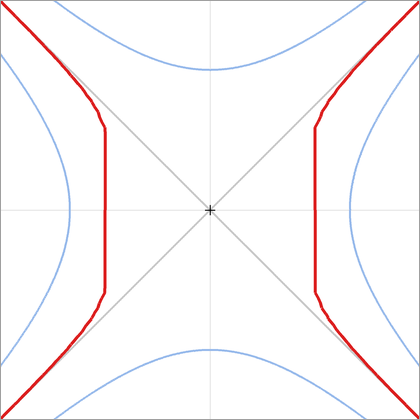
\includegraphics[width=0.2\textwidth]{pictures/report/interp/interp_A1_1_vertex_mid_from_minus.png} &
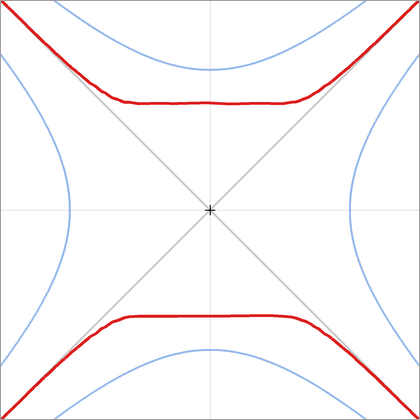
\includegraphics[width=0.2\textwidth]{pictures/report/interp/interp_A1_1_vertex_mid_from_plus.png} &
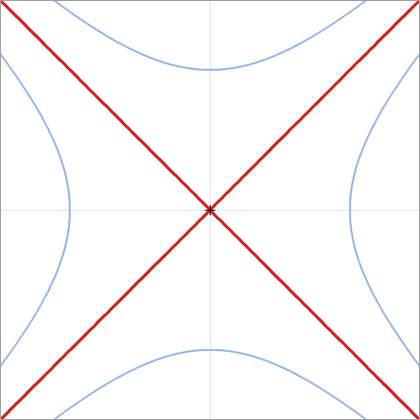
\includegraphics[width=0.2\textwidth]{pictures/report/interp/interp_A1_1_sdf_average.png} &
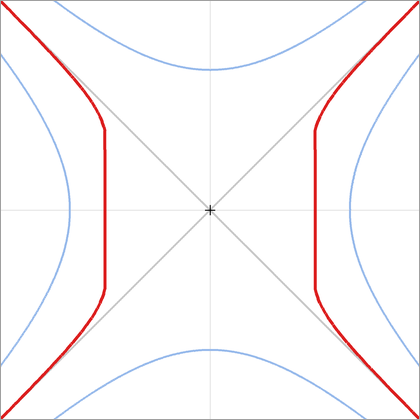
\includegraphics[width=0.2\textwidth]{pictures/report/interp/interp_A1_1_exact_vertex_mid.png} \\
\rotatebox{90}{\scriptsize\ \ \ $x^2+y^2-z^2+xyz$, $G=x$} &
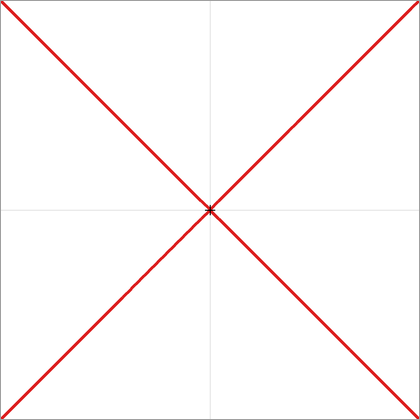
\includegraphics[width=0.2\textwidth]{pictures/report/interp/interp_A1_x_vertex_mid_from_minus.png} &
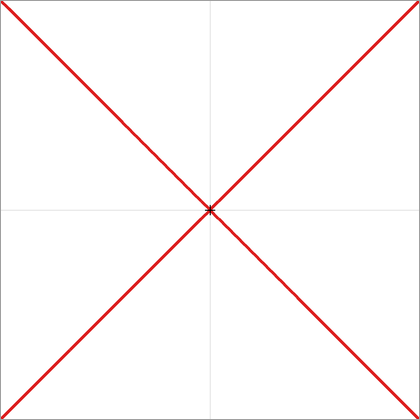
\includegraphics[width=0.2\textwidth]{pictures/report/interp/interp_A1_x_vertex_mid_from_plus.png} &
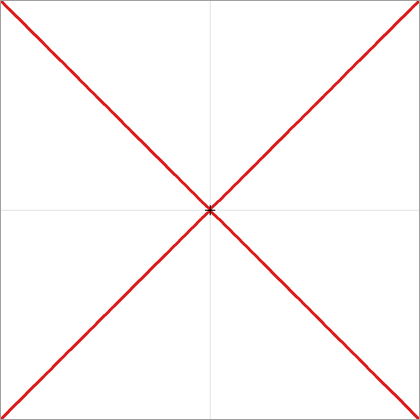
\includegraphics[width=0.2\textwidth]{pictures/report/interp/interp_A1_x_sdf_average.png} &
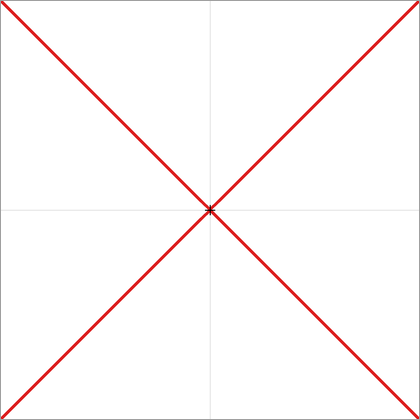
\includegraphics[width=0.2\textwidth]{pictures/report/interp/interp_A1_x_exact_vertex_mid.png} \\
\rotatebox{90}{\scriptsize\ \ \ \ \ \ \ $x^2+y^2+z^3$, $G=x$} &
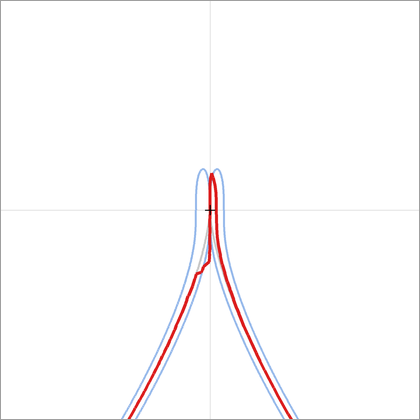
\includegraphics[width=0.2\textwidth]{pictures/report/interp/interp_A2a_x_vertex_mid_from_minus.png} &
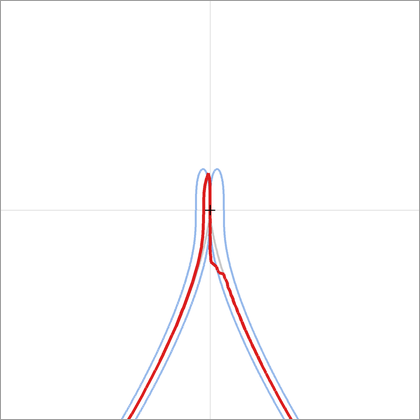
\includegraphics[width=0.2\textwidth]{pictures/report/interp/interp_A2a_x_vertex_mid_from_plus.png} &
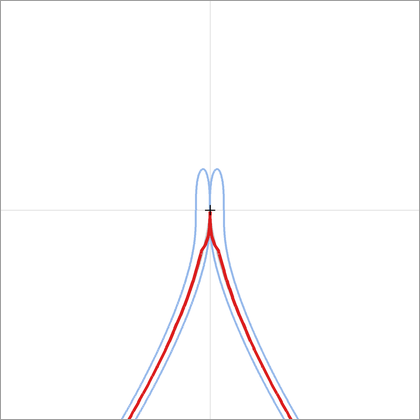
\includegraphics[width=0.2\textwidth]{pictures/report/interp/interp_A2a_x_sdf_average.png} &
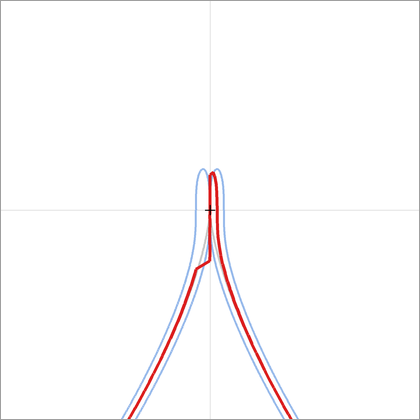
\includegraphics[width=0.2\textwidth]{pictures/report/interp/interp_A2a_x_exact_vertex_mid.png} \\
\rotatebox{90}{\scriptsize\ \ \ \ \ \ \ $x^3+y^3+z^3$, $G=x$} &
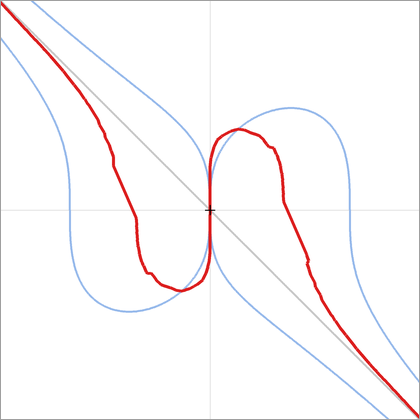
\includegraphics[width=0.2\textwidth]{pictures/report/interp/interp_E6a_x_vertex_mid_from_minus.png} &
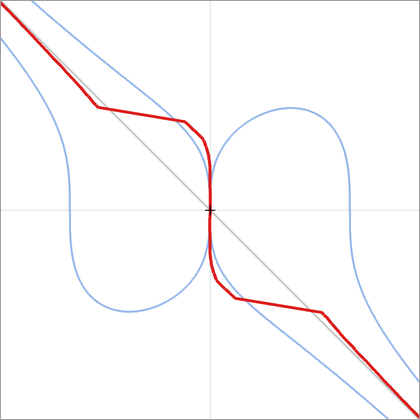
\includegraphics[width=0.2\textwidth]{pictures/report/interp/interp_E6a_x_vertex_mid_from_plus.png} &
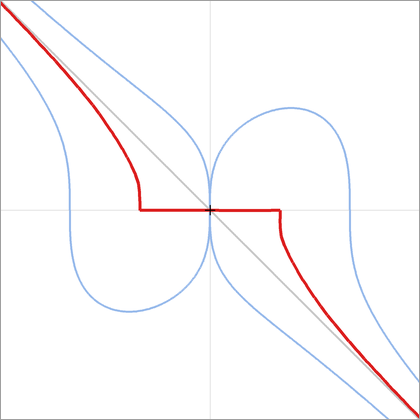
\includegraphics[width=0.2\textwidth]{pictures/report/interp/interp_E6a_x_sdf_average.png} &
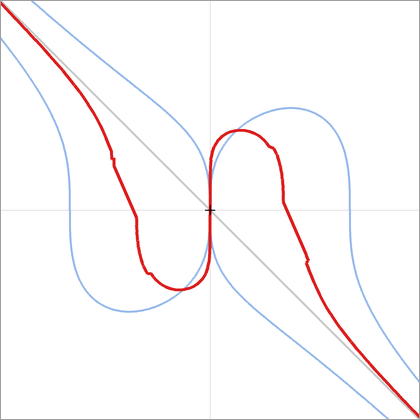
\includegraphics[width=0.2\textwidth]{pictures/report/interp/interp_E6a_x_exact_vertex_mid.png} \\
\end{tabular}
\caption{Slices of the reconstructions of $S_0$ through $P$ for $\varepsilon=0.01$,
$N=128$ (planes $x=0$, $x=0$, $y=0$, $z=0$; window $[-0.15,0.15]^2$). Light blue:
the exact $S_{-\varepsilon}$ and $S_{+\varepsilon}$; grey: the exact $S_0$; red:
the reconstruction. Row 1: the vertex interpolations keep the topology of their
source (one sheet with a waist, two separate sheets) and miss the pinch at $P$; the
SDF interpolation is the cone. Row 2: the deformation is a shift by $\pm k/2$,
which cancels: all reconstructions are the cone. Row 3: the spike is in both
$S_{\pm\varepsilon}$ and stays. Row 4: different shapes on the two sides; no
reconstruction is correct near $P$.}
\label{fig:interp-slices}
\end{figure}

Table~\ref{tab:interp-topology} counts, over the $200$ runs at $N=128$, how often the reconstruction has the same number of components and the same Euler characteristic in $Q$ as the direct mesh of $F$. The vertex interpolations agree exactly as often as their source meshes do ($163$ against $164$ for $S_{-\varepsilon}$, $184$ against $185$ for $S_{+\varepsilon}$): they inherit the topology of the source, as expected in Section~\ref{sec:r-interp-theory}. Where the topologies differ, it is the perturbation that changed them, for example $G=1$ on the double point ($S_{-\varepsilon}$ is one sheet with $\chi=0$, $S_0$ two cones with $\chi=2$ in the mesh of $F$), $G=1$ on $x^2+y^3-3yz^2$ (one sheet instead of three) or $G=x+y$ on $x^3+y^3+z^2+x^2$ (two components instead of one). In addition, the vertex interpolation folds the mesh near $P$ (flipped triangles) in $40$--$50\%$ of the runs. The SDF interpolation has the topology of the mesh of $F$ in $197$ of the $200$ runs and never folds; it is the only one of the three that can create or remove a pinch. No reconstruction had holes.

\begin{table}[!ht]
\centering
\small
\begin{tabular}{l c c c}
\toprule
& \makecell{same topology\\as mesh of $F$}
& \makecell{runs with\\flipped triangles}
& \makecell{runs with\\non-manifold edges} \\
\midrule
mesh of $S_{-\varepsilon}$ & 164 & -- & 0 \\
mesh of $S_{+\varepsilon}$ & 185 & -- & 1 \\
vertex interpolation from $S_{-\varepsilon}$ & 163 & 79 & 0 \\
vertex interpolation from $S_{+\varepsilon}$ & 184 & 81 & 1 \\
vertex interpolation (exact) & 163 & 102 & 0 \\
SDF interpolation & 197 & -- & 3 \\
\bottomrule
\end{tabular}
\caption[Interpolation: topology]{Topology of the reconstructions inside $Q$ over the $200$ runs at $N=128$ ($40$ pairs, $5$ values of $\varepsilon$). ``Same topology'': the same number of connected components and the same Euler characteristic as the direct Marching Cubes mesh of $F$.}
\label{tab:interp-topology}
\end{table}

The grid resolution changes the picture only for the direct mesh. The median error at $\varepsilon=10^{-3}$ over the $40$ pairs is
\begin{center}
\small
\begin{tabular}{c c c c c c}
\toprule
$N$ & direct mesh of $F$ & $S_{\pm\varepsilon}$ & vertex (mesh) & vertex (exact) & SDF \\
\midrule
32  & 0.0080 & 0.018 & 0.012 & 0.012 & 0.0084 \\
64  & 0.0041 & 0.021 & 0.015 & 0.012 & 0.0066 \\
128 & 0.0021 & 0.021 & 0.016 & 0.012 & 0.0043 \\
\bottomrule
\end{tabular}
\end{center}
The direct mesh of $F$ improves with the grid. The endpoints and the vertex interpolations do not: their error is the actual difference between the interpolated and the singular surface near $P$, which a finer grid only shows more clearly. The SDF interpolation improves with $N$, but more slowly than the direct mesh.

In summary, linear interpolation between $S_{-\varepsilon}$ and $S_{+\varepsilon}$ reconstructs $S_0$ to second order away from the singular point: the first-order changes of the two sides cancel, and already for $\varepsilon=10^{-3}$ the error there is that of a direct mesh. Near the singular point it does not: the two sides of the deformation are different shapes of size $\lambda(\varepsilon)$, nothing cancels, and the error decreases with the same rate $\varepsilon^\alpha$ as for $S_{\pm\varepsilon}$ alone. Vertex interpolation cannot change the topology, so it never recreates the singular point when the perturbation removed it, and it often folds the mesh near $P$. Interpolating distance fields can recreate the singular point, but reliably only when the deformation is symmetric with respect to $S_0$. Interpolating the implicit functions is exact, but returns the original problem of meshing $\{F=0\}$.

% -----------------------------------------------------------------------------
\section{The Weighted Cone Patch}
\label{sec:r-cone-results}

The three reconstructions of Section~\ref{sec:r-cone} (the singular cone patch, the hybrid and the gradient-line correspondence) were added to the experiment of Section~\ref{sec:r-interp-setup}: the same $40$ pairs, five values of $\varepsilon$ and three grids, measured against the exact $S_0$ in the same way.

\subsection{Comparison with Marching Cubes}

The cone patch uses only $F$, so it does not depend on $G$ or $\varepsilon$. Table~\ref{tab:cone-vs-mc} compares it with the direct Marching Cubes mesh of $F$ for every surface. Near $P$ the error is smaller on every surface and at every resolution. At $N=128$ the median over the surfaces drops from $0.0021$ to $0.00055$, a factor of about $4$, and for the double cone and the Fermat cones by a factor of $7$. Away from $P$ both meshes are the same ($0.00031$). The topology is correct, with one component and $\chi=1$, in all $600$ runs, while Marching Cubes of $F$ is wrong in every run on exactly two surfaces. On the double cone the two nappes do not touch at $P$ ($2$ components, $\chi=2$), and on $x^2+y^3-3yz^2$ the three pieces stay separate ($3$ components, $\chi=3$). On these two surfaces the patch finds two and three loops, one for each component of the link, and joins them at $P$.

\begin{table}[!ht]
\centering
\small
\begin{adjustbox}{max width=\textwidth}
\begin{tabular}{l l c c c c c c c c c}
\toprule
& & \multicolumn{2}{c}{$N=32$} & \multicolumn{2}{c}{$N=64$} & \multicolumn{2}{c}{$N=128$} & \multicolumn{2}{c}{components$/\chi$} & \\
\cmidrule(lr){3-4}\cmidrule(lr){5-6}\cmidrule(lr){7-8}\cmidrule(lr){9-10}
type & $F$ & MC & patch & MC & patch & MC & patch & MC & patch & loops \\
\midrule
$A_1$ & $x^2+y^2-z^2+xyz$ & 0.0058 & 0.00041 & 0.0029 & 0.00031 & 0.0014 & 0.00021 & 2/2 & 1/1 & 2 \\
$A_2$ & $x^2+y^2+z^3$ & 0.0073 & 0.00062 & 0.0041 & 0.00037 & 0.0021 & 0.00055 & 1/1 & 1/1 & 1 \\
$A_2$ & $x^2-y^2+z^3$ & 0.0059 & 0.00032 & 0.0029 & 0.00032 & 0.0015 & 0.00028 & 1/1 & 1/1 & 1 \\
$A_2$ & $x^3+y^3+z^2+x^2$ & 0.0074 & 0.00061 & 0.0041 & 0.00039 & 0.0021 & 0.00055 & 1/1 & 1/1 & 1 \\
$D_4$ & $x^2+y^3+z^3$ & 0.0061 & 0.0019 & 0.0031 & 0.00084 & 0.0015 & 0.00074 & 1/1 & 1/1 & 1 \\
$D_4$ & $x^2+y^3-3yz^2$ & 0.0109 & 0.0021 & 0.0054 & 0.0042 & 0.0027 & 0.00087 & 3/3 & 1/1 & 3 \\
$\tilde E_6$ & $x^3+y^3+z^3$ & 0.0075 & 0.00062 & 0.0037 & 0.00051 & 0.0019 & 0.00028 & 1/1 & 1/1 & 1 \\
$\tilde E_6$ & $x^3+y^3-z^3$ & 0.0075 & 0.00062 & 0.0037 & 0.00051 & 0.0019 & 0.00028 & 1/1 & 1/1 & 1 \\
$\tilde E_6$ & $x^3+y^3+z^3+xyz$ & 0.0107 & 0.0016 & 0.0053 & 0.0012 & 0.0027 & 0.00058 & 1/1 & 1/1 & 1 \\
$\tilde E_6$ & $x^3+2y^3+3z^3+2xyz$ & 0.0122 & 0.0015 & 0.0061 & 0.0012 & 0.0030 & 0.00068 & 1/1 & 1/1 & 1 \\
\bottomrule
\end{tabular}
\end{adjustbox}
\caption[Cone patch against Marching Cubes]{Local Hausdorff distance to the exact
$S_0$ near $P$ ($\|p\|_\infty<0.06$) of the direct Marching Cubes mesh of $F$ (MC)
and of the singular cone patch, and the topology inside $Q$ (number of components and
Euler characteristic; correct is $1/1$). ``Loops'': components of the link found by
the patch.}
\label{tab:cone-vs-mc}
\end{table}

\begin{figure}[!ht]
\centering
\setlength{\tabcolsep}{2pt}
\begin{tabular}{c c c c}
MC of $F$ & cone patch & MC of $F$ & cone patch \\
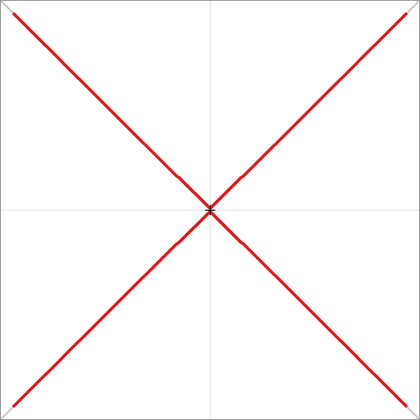
\includegraphics[width=0.22\textwidth]{pictures/report/interp/interp_A1_1_direct_S0_zoom.png} &
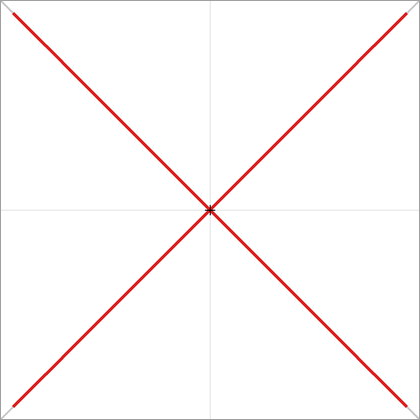
\includegraphics[width=0.22\textwidth]{pictures/report/interp/interp_A1_1_singular_cone_zoom.png} &
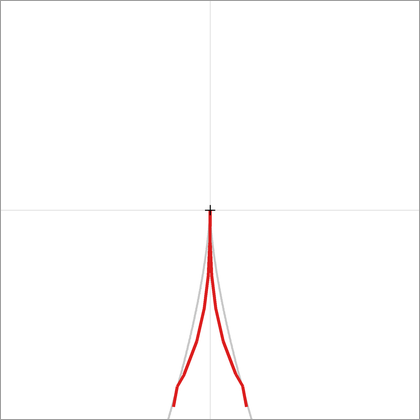
\includegraphics[width=0.22\textwidth]{pictures/report/interp/interp_A2a_x_direct_S0_zoom.png} &
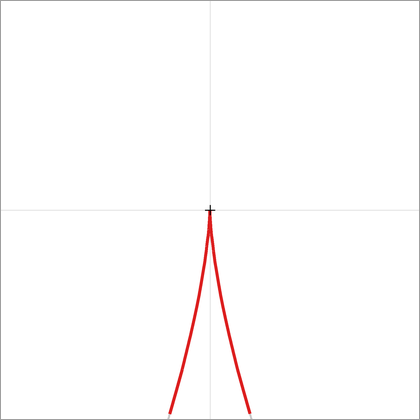
\includegraphics[width=0.22\textwidth]{pictures/report/interp/interp_A2a_x_singular_cone_zoom.png} \\
\multicolumn{2}{c}{\small $x^2+y^2-z^2+xyz$, plane $x=0$} & \multicolumn{2}{c}{\small $x^2+y^2+z^3$, plane $y=0$}
\end{tabular}
\caption{Close-ups of $S_0$ around $P$ (window $[-0.04,0.04]^2$, about $13$ cells at
$N=128$). Grey: the exact $S_0$; red: the mesh.}
\label{fig:cone-zoom}
\end{figure}

Figure~\ref{fig:cone-zoom} shows the difference on the scale of the grid. For the double cone, Marching Cubes leaves small steps next to $P$ and does not join the two lines, while the patch crosses exactly at $P$. For the horn, Marching Cubes follows the tip only roughly and stops short of it, because the tip is thinner than a cell; the patch follows it into $P$. This is why the box radius depends on the weights (Section~\ref{sec:r-cone-algorithm}). For the horn, with $w=(\tfrac12,\tfrac12,\tfrac13)$, the tip is thinner than two cells up to the distance $(2h)^{2/3}\approx0.054$ from $P$ at $N=128$, so the box must reach that far; with the fixed radius $4h=0.025$ the error near $P$ was still $0.0018$. For equal weights the radius stays $4h$.

The error of the patch near $P$ does not decrease regularly with $h$: the median order between $N=64$ and $N=128$ is $0.8$, against $1.0$ for Marching Cubes. It is now made of the Marching Cubes triangles just outside the box and of the long thin triangles of the rings, and the box radius changes with $h$. It stays below the error of Marching Cubes on the same grid in every case.

\subsection{All Reconstructions Together}

Table~\ref{tab:cone-median} extends Table~\ref{tab:interp-median} by the three new methods, and Table~\ref{tab:cone-topology} compares the topology of all reconstructions with the true topology of $S_0\cap Q$.

The hybrid, which uses the interpolation of $S_{\pm\varepsilon}$ away from $P$ and the cone patch near $P$ and does not use $F$, is the only reconstruction from $S_{\pm\varepsilon}$ whose error near $P$ does not decrease only like $\varepsilon^\alpha$. From $\varepsilon=10^{-2.5}$ on it is $0.0004$--$0.0007$, against $0.0067$--$0.027$ for the vertex interpolation, and below the error of the direct mesh of $F$. At $\varepsilon=10^{-2}$ the deformation reaches across the whole box $Q$, the box of the patch ($0.24$) is larger than $Q$, and the error comes from the loop, which lies where the interpolation is still poor ($0.0038$ near $P$, $0.013$ away). The hybrid is within twice the error of the direct mesh in $19$, $33$ and $40$ of the $40$ pairs for $\varepsilon=10^{-2},10^{-3},10^{-4}$ (the vertex interpolation in $6$, $19$ and $23$), and it has the correct topology in $599$ of the $600$ runs.

The gradient-line correspondence improves the vertex interpolation away from $P$, most at $\varepsilon=10^{-2}$ ($0.0083$ against $0.037$), because it follows the normal expansion of Proposition~\ref{prop:second-order} instead of approximating it. Over the $200$ runs at $N=128$ it is better than the closest point in $45$ and worse in $8$. Near $P$ it does not help, giving the same rate as the endpoints, and it folds the mesh \emph{more} often ($138$ of $200$ runs, against $102$ for the exact vertex interpolation). Close to $P$ the gradient of $F$ is small and changes direction quickly (Section~\ref{sec:poly-quality}), neighbouring vertices follow very different lines, and where the line misses $S_{+\varepsilon}$ the closest point is used instead. The folding of the vertex interpolation is therefore a property of the region near $P$, not of the choice of correspondence.

\begin{table}[!ht]
\centering
\small
\begin{adjustbox}{max width=\textwidth}
\begin{tabular}{l c c c c c c c c c c}
\toprule
& \multicolumn{5}{c}{near $P$} & \multicolumn{5}{c}{away from $P$} \\
\cmidrule(lr){2-6}\cmidrule(lr){7-11}
$\varepsilon$ & $10^{-2}$ & $10^{-2.5}$ & $10^{-3}$ & $10^{-3.5}$ & $10^{-4}$ & $10^{-2}$ & $10^{-2.5}$ & $10^{-3}$ & $10^{-3.5}$ & $10^{-4}$ \\
\midrule
direct mesh of $F$ & 0.0021 & 0.0021 & 0.0021 & 0.0021 & 0.0021 & 0.0003 & 0.0003 & 0.0003 & 0.0003 & 0.0003 \\
vertex interpolation (exact) & 0.048 & 0.023 & 0.012 & 0.0067 & 0.0037 & 0.037 & 0.0022 & 0.0005 & 0.0003 & 0.0003 \\
vertex interp.\ along $\nabla F$ & 0.032 & 0.019 & 0.011 & 0.0064 & 0.0033 & 0.0083 & 0.0013 & 0.0004 & 0.0003 & 0.0003 \\
SDF interpolation & 0.0095 & 0.0064 & 0.0043 & 0.0038 & 0.0026 & 0.0060 & 0.0018 & 0.0007 & 0.0007 & 0.0004 \\
hybrid (interp.\ + cone patch) & 0.0038 & 0.0006 & 0.0007 & 0.0004 & 0.0004 & 0.013 & 0.0007 & 0.0005 & 0.0003 & 0.0003 \\
singular cone patch & 0.0006 & 0.0006 & 0.0006 & 0.0006 & 0.0006 & 0.0003 & 0.0003 & 0.0003 & 0.0003 & 0.0003 \\
\bottomrule
\end{tabular}
\end{adjustbox}
\caption[Reconstructions including the cone patch: median errors]{As
Table~\ref{tab:interp-median} ($N=128$, median over the $40$ pairs), with the
gradient-line correspondence, the hybrid and the singular cone patch.}
\label{tab:cone-median}
\end{table}

\begin{table}[!ht]
\centering
\small
\begin{tabular}{l c c}
\toprule
& \makecell{correct topology\\(1 component, $\chi=1$)} & \makecell{runs with\\flipped triangles} \\
\midrule
direct mesh of $F$ & 160 & -- \\
meshes of $S_{-\varepsilon}$ / $S_{+\varepsilon}$ & 143 / 151 & -- \\
vertex interpolation (mesh, from $S_{-\varepsilon}$) & 142 & 79 \\
vertex interpolation (exact) & 142 & 102 \\
vertex interpolation along $\nabla F$ & 139 & 138 \\
SDF interpolation & 157 & -- \\
hybrid (interpolation + cone patch) & 200 & -- \\
singular cone patch & 200 & -- \\
\bottomrule
\end{tabular}
\caption[Topology against the cone over the link]{Topology inside $Q$ over the $200$
runs at $N=128$, compared with the true topology of $S_0\cap Q$ (a cone, hence one
component and $\chi=1$), not with the mesh of $F$ as in Table~\ref{tab:interp-topology}.}
\label{tab:cone-topology}
\end{table}

\begin{figure}[!ht]
\centering
\setlength{\tabcolsep}{2pt}
\begin{tabular}{l c c c}
& vertex (exact) & along $\nabla F$ & hybrid \\
\rotatebox{90}{\scriptsize\ \ \ $x^2+y^2-z^2+xyz$, $G=1$} &
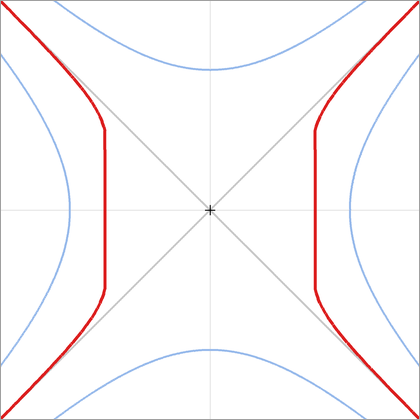
\includegraphics[width=0.24\textwidth]{pictures/report/interp/interp_A1_1_exact_vertex_mid.png} &
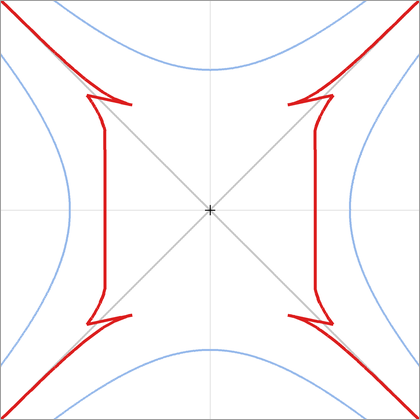
\includegraphics[width=0.24\textwidth]{pictures/report/interp/interp_A1_1_normal_mid.png} &
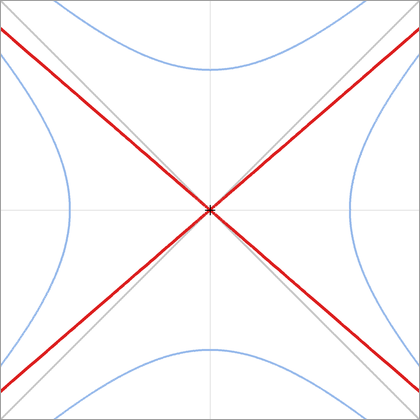
\includegraphics[width=0.24\textwidth]{pictures/report/interp/interp_A1_1_hybrid_cone.png} \\
\rotatebox{90}{\scriptsize\ \ \ \ \ \ \ $x^3+y^3+z^3$, $G=x$} &
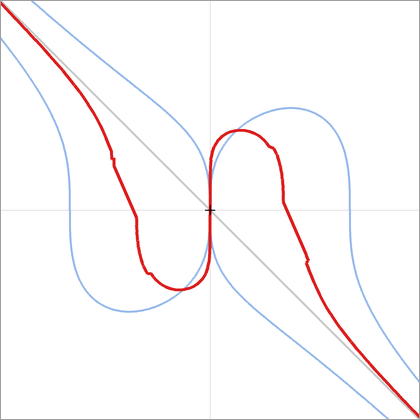
\includegraphics[width=0.24\textwidth]{pictures/report/interp/interp_E6a_x_exact_vertex_mid.png} &
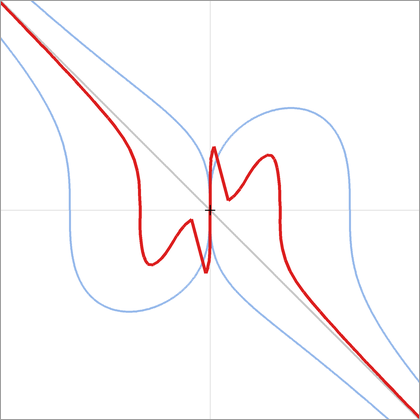
\includegraphics[width=0.24\textwidth]{pictures/report/interp/interp_E6a_x_normal_mid.png} &
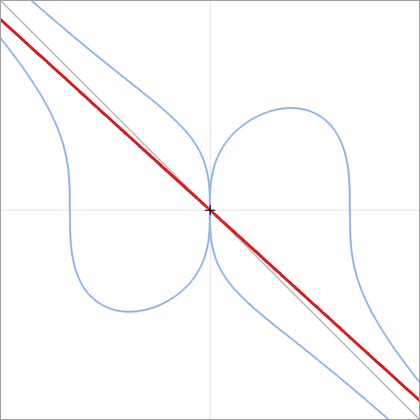
\includegraphics[width=0.24\textwidth]{pictures/report/interp/interp_E6a_x_hybrid_cone.png} \\
\end{tabular}
\caption{Reconstructions from $S_{\pm\varepsilon}$, $\varepsilon=0.01$, $N=128$, as in
Figure~\ref{fig:interp-slices}. The hybrid passes through $P$ and has the shape of
$S_0$ even where the two sides are very different.}
\label{fig:cone-slices}
\end{figure}

The weighted cone patch is thus a voxel method that models the neighbourhood of an isolated singular point faithfully. Away from $P$ it is Marching Cubes, and near $P$ the surface is rebuilt from its own boundary curve with the scaling that the singularity itself defines. It gives the topology of the cone over the link in every run, puts $P$ into the mesh as a vertex, and reduces the error near $P$ by a factor of about $4$ (up to $7$). It applies to isolated singular points with a non-degenerate quasi-homogeneous principal part (Definition~\ref{def:sqh}). The same patch completes the linear interpolation of $S_{-\varepsilon}$ and $S_{+\varepsilon}$: the interpolation is used where it is of second order, away from $P$, and the patch replaces it where it cannot work.

% =============================================================================
\chapter*{Conclusion}
\addcontentsline{toc}{chapter}{Conclusion}
\label{ch:conclusion}
% =============================================================================

The aim of this thesis was to develop a voxel method for extracting an isosurface given by a polynomial that models the neighbourhood of a singular point faithfully, to describe the class of algebraic surfaces on which it works reliably, and to evaluate it against existing extraction algorithms with respect to geometric accuracy and topological correctness.

Chapters~\ref{ch:implicit} and~\ref{ch:extraction} collected the necessary background: implicit surfaces and their singular points, the local invariants and normal forms of isolated singularities, the conic structure theorem, and the classical extraction methods, Marching Cubes, Marching Tetrahedra and Dual Contouring. Section~\ref{sec:poly-quality} explained how these methods behave near a singular point. A singular point that is not on a grid edge is never a vertex of a Marching Cubes mesh, parts of the surface thinner than a cell disappear, and the known topological guarantees refer to the trilinear interpolant, which near a singular point can have the wrong topology.

Chapter~\ref{ch:theory} studied what happens to an isolated singular point under a perturbation $F+kG$. A scaling argument based on the weights of the singularity predicts the rate at which $S_k$ approaches $S_0$, and for homogeneous $F$ and $G$ the prediction is exact (Proposition~\ref{prop:self-similar}). The Tjurina algebra separates the perturbations that genuinely change the singularity from those that only move it, and the conservation of the Milnor number bounds the number of singular points that can appear. For the diagonal cubic cones and linear perturbations all singular points were found in closed form (Proposition~\ref{prop:linear}).

Chapter~\ref{ch:experiments} tested these predictions on $144$ pairs of surfaces and perturbations. The rate is decided by the singularity type and by the order of $G$: for the cubic cones it is exactly $1/(3-m)$, and for the other types it lies in the predicted range, with the end of the range decided by the sign of $k$ and by the real shape of the surface. $253$ of the $268$ measured rates agree with the prediction, and the remaining $15$ are explained either by two effects being visible at once or by the resolution of the measurement. What happens at the singular point was decided by $G(P)$ and $\nabla G(P)$ in every pair. Inessential perturbations mostly move the surface, but their second-order effect can still be visible, like the thin spike of the horn cusp. New singular points are rare and predictable: they appear only for special directions of $G$ or for quadratic $G$ with indefinite signs, and the computed multiplicities always agree with the Milnor number.

Two approaches to a faithful extraction were then compared. Linear interpolation between $S_{-\varepsilon}$ and $S_{+\varepsilon}$ reconstructs $S_0$ to second order away from the singular point, but not near it, where the error decreases only with the same rate $\varepsilon^\alpha$ as for $S_{\pm\varepsilon}$ alone; averaging the implicit functions is exact, but it gives back the original problem. The method proposed in this thesis, the weighted cone patch of Section~\ref{sec:r-cone}, keeps the Marching Cubes mesh away from $P$ and rebuilds the surface inside a small box around $P$ from scaled copies of its own boundary curve, using the weighted scaling of the singularity. It applies to isolated singular points with a non-degenerate quasi-homogeneous principal part, the semi-quasihomogeneous singularities (Definition~\ref{def:sqh}), which include all simple singularities and all ten test surfaces; the current implementation covers principal parts of degree at most three. Compared with Marching Cubes on the same grid, it gave the correct topology in all $600$ runs, where Marching Cubes failed for the double cone and the three-line $D_4$ point, it contains the singular point as a mesh vertex, and it reduced the error near the singular point by a factor of about $4$, up to $7$. Combined with the interpolation, the same patch also reconstructs $S_0$ from $S_{\pm\varepsilon}$ near $P$, with the correct topology in $599$ of $600$ runs.

\section*{Future Work}

Several directions follow from the results. The weighted cone patch resolves the neighbourhood of one known isolated singular point with a principal part of degree at most three, and it can be extended in four ways. First, the stationary-point search of Section~\ref{sec:r-method} already finds the singular points of $S_0$, so the patch can be applied at each of them automatically, with boxes that do not overlap. Second, reading the Taylor coefficients beyond degree three would cover $A_k$ for $k\ge3$, $D_k$ for $k\ge5$ and $E_6$, $E_7$, $E_8$, which are all quasi-homogeneous. Third, for unequal weights the rings shrink faster across the horn than along it, and the triangles near $P$ become long and thin; fewer vertices on the smaller rings would keep them well shaped. Fourth, along a curve of singular points, for example for the Whitney umbrella $x^2-y^2z$, the conic structure holds in the planes transversal to the curve, and a patch shaped like a tube around the curve is a natural generalisation.

The evaluation can also be extended. In this thesis the proposed method was compared with Marching Cubes; a comparison with Dual Contouring \cite{ju2002dual}, with Marching Cubes 33 \cite{chernyaev1995marching,lewiner2003efficient} and with adaptive methods \cite{frisken2000adaptively} on the same surfaces and with the same measures would show how much of the improvement is specific to the singular point. Finally, the perturbations used in the experiments were selected from a fixed list. A basis of the Tjurina algebra can be used to select perturbation directions systematically, with the basis elements and their combinations as perturbations and inessential perturbations as controls, to study how the independent deformation directions influence the rates, the singular points and the reconstruction of the singular surface.





% Use \input{} to insert your own numbered chapters (e.g. Basic notions, Results, Conclusion)
%
% \input{01-basic-notions.tex}
%

\newpage

% after the main part of the thesis and conclusion you include the bibliography, which is stored in the "bibliography.bib" file

\bibliographystyle{alpha} % we use Surname/year format for references, e.g. Boris Delaunay, ..., 1934 = [Del34]
\bibliography{bibliography} % include the reference file

% =============================================================================
% NOTES FOR LUCIA (not part of the thesis, everything below is commented out)
% =============================================================================
\begin{comment}
Is this enough for a master's thesis?
  The structure now follows the annotation (zadanie): overview of methods and
  their behaviour near singularities (Ch. 2, Sec. 2.5), a voxel method that
  models the neighbourhood of the singularity (Sec. 4.2, weighted cone patch),
  the class of surfaces where it works (Sec. 4.2.2, semi-quasihomogeneous),
  and an evaluation with geometric and topological measures (Ch. 5).
  Content-wise this is enough for a master's thesis, with ONE real gap:

  1. The annotation says "compare with existing algorithms" (plural). Right
     now the method is compared only with Marching Cubes. This is the most
     important thing to add. Suggestion, in this order:
       a) Dual Contouring (Ch. 2 already explains it; Hermite data are easy
          to get since F is a polynomial and we have exact gradients),
       b) Marching Cubes 33 / Lewiner (e.g. compare against the "lewiner"
          variant of scikit-image's marching_cubes on the same grid),
       c) plain adaptive refinement near P (refine the grid around P by 2x,
          4x, 8x): this answers the obvious question of a reviewer, "why not
          just use a finer grid near P?".
     Then add one table to Sec. 5.10 with the same columns as
     Table "Cone patch against Marching Cubes" (error near P, components/chi).

  2. Still to write: Introduction (00-intro.tex is empty), Abstract and
     Abstrakt (intro.tex has placeholders), Acknowledgement.

  3. Figures I would add (tell me and I can make the TikZ ones):
       - a schematic of the cone patch: box B, boundary loop, rings, apex P
         (TikZ, for Sec. 4.2.3 next to Algorithm 1);
       - 3D screenshots from the viewer of the cone patch mesh on the horn
         and on x^2+y^3-3yz^2 (three loops joined at P);
       - one log-log plot of d(k) against |k| with the fitted line, e.g. for
         x^2+y^2+z^3 with G=z (both signs), to show how alpha is measured
         (the data are in experiments_thesis/.../exact_geometry.csv);
       - a 3D picture of the Whitney umbrella for Sec. 1.3.1 (optional).

  4. Bibliography: please check the new entries at the end of
     bibliography.bib (milnor1970isolated, arnold1985singularities,
     hatcher2002algebraic, edelsbrunner2010computational, jones2006distance,
     plantinga2004isotopic, stander1997guaranteeing). I also fixed the
     author of arnold2012singularities (it was "Arnold, Elionora"; the book
     is by Vladimir I. Arnold). The classification results (normal forms,
     semi-quasihomogeneous) are in VOLUME 1, so they cite the new
     arnold1985singularities entry.

  5. Optional: if the supervisor wants all ten surfaces in detail, the full
     tables of the other six surfaces from report.tex can go into an
     appendix without any change.

  6. The old drafts ch3.tex, ch4.tex, ch5.tex, cap3_4.tex are no longer used
     and can be moved to old/.
\end{comment}

\end{document}
